% =====================================================================
%  CeNTREX State Cleanup
%  Thesis-format summary of the design and optical-Bloch simulations of the two
%  rotational-state cleanup stages of CeNTREX: CU1 (X, J=1) and CU2 (X, J=2)
%  Compile: latexmk -pdf main.tex   (or the LaTeX Workshop default recipe)
%  Figures are not yet included: every figure is a framed placeholder that names
%  the file it expects in figures/ and the notebook / HDF5 run / slide it comes from.
% =====================================================================
\documentclass[11pt,a4paper,oneside]{report}

\usepackage[T1]{fontenc}
\usepackage{lmodern}
\usepackage[a4paper,left=30mm,right=25mm,top=28mm,bottom=28mm]{geometry}
\usepackage{setspace}
\onehalfspacing
\usepackage{amsmath,amssymb,bm}
\usepackage{graphicx}
\usepackage{booktabs,tabularx,multirow,array}
\newcolumntype{L}{>{\raggedright\arraybackslash}X}  % ragged-right X column
\usepackage[separate-uncertainty=true]{siunitx}
\DeclareSIUnit{\gauss}{G}
\usepackage{xcolor}
\usepackage[font=small,labelfont=bf]{caption}
\usepackage{subcaption}
\usepackage{float}
\usepackage{enumitem}
\setlist{itemsep=2pt,topsep=4pt}
\usepackage{fancyhdr}
\usepackage[nottoc]{tocbibind}
\usepackage[hidelinks]{hyperref}
\graphicspath{{figures/}}
\setlength{\emergencystretch}{3em}
% compact chapter headings (report default leaves ~170pt above the text)
\usepackage{titlesec}
\titleformat{\chapter}[display]{\normalfont\huge\bfseries\filright\hyphenpenalty=10000}{\chaptertitlename\ \thechapter}{10pt}{\Huge}
\titlespacing*{\chapter}{0pt}{0pt}{20pt}
% float placement: allow more floats per text page, fewer sparse float pages
\renewcommand{\topfraction}{0.9}
\renewcommand{\bottomfraction}{0.8}
\renewcommand{\textfraction}{0.07}
\renewcommand{\floatpagefraction}{0.85}
\setcounter{topnumber}{3}
\setcounter{bottomnumber}{2}
\setcounter{totalnumber}{5}
% float-only pages start at the top instead of being centred vertically
\makeatletter
\setlength{\@fptop}{0pt}
\setlength{\@fpsep}{14pt plus 4pt}
\setlength{\@fpbot}{0pt plus 1fil}
\makeatother

\pagestyle{fancy}
\fancyhf{}
\fancyhead[L]{\small\nouppercase{\leftmark}}
\fancyhead[R]{\small\thepage}
\renewcommand{\headrulewidth}{0.4pt}
\fancypagestyle{plain}{\fancyhf{}\fancyfoot[C]{\small\thepage}\renewcommand{\headrulewidth}{0pt}}

% ---- notation ---------------------------------------------------------
\newcommand{\code}[1]{\texttt{#1}}
\newcommand{\etac}{\eta_{\mathrm{c}}}
\newcommand{\Ngam}{N_{\gamma}}
\newcommand{\sigs}{\sigma_{s}}
\newcommand{\sigy}{\sigma_{y}}
\newcommand{\wmod}{\omega_{\mathrm{m}}}
\newcommand{\wpol}{\omega_{\mathrm{p}}}
\newcommand{\Dxb}{D_{XB}}
\newcommand{\fAOM}{f_{\mathrm{AOM}}}
\newcommand{\Dmain}{\Delta_{\mathrm{main}}}

% ---- figure placeholder -------------------------------------------------
% \figplaceholder[height]{expected file name}
% Replace by \includegraphics[width=\textwidth]{<file>} once the figure exists.
\newcommand{\figplaceholder}[2][0.30\textheight]{%
  \fbox{\begin{minipage}[c][#1][c]{0.95\textwidth}\centering
    {\color{gray}\Large Figure placeholder\par}\vspace{2mm}
    {\color{gray}\small\texttt{figures/\detokenize{#2}}\par}
  \end{minipage}}}

\begin{document}

% =====================================================================
\begin{titlepage}
\centering
\vspace*{25mm}
{\Huge\bfseries CeNTREX State Cleanup\par}
\vspace{10mm}
{\Large Design and optical-Bloch-equation simulations of the\\[2mm]
rotational-state cleanup stages CU1 ($J=1$) and CU2 ($J=2$)\par}
\vspace{30mm}
{\large Yuanhang Yang\par}
\vspace{4mm}
{\large CeNTREX Collaboration\par}
\vfill
{\large October 2026\par}
\vspace{10mm}
\end{titlepage}

% =====================================================================
\pagenumbering{roman}
\chapter*{Abstract}
\addcontentsline{toc}{chapter}{Abstract}

The CeNTREX experiment measures the Schiff moment of the $^{205}$Tl nucleus in a beam of
thallium fluoride. After the electrostatic lens the molecules are in $X(v{=}0)$, $J=2$, and
state preparation (SPB) transfers them to $J=1$, the level used in the interaction region.
Two state-cleanup stages bracket this transfer: CU1 removes the population of $J=1$ before
SPB, and CU2 removes the population left in $J=2$ after it. Both stages pump the molecules
through the $B\,{}^3\Pi_1$ state into other rotational levels, in the electric field that is
kept on to preserve the spin. In that field the Stark interaction spreads the excited-state
sublevels over tens of MHz, so that a single laser frequency leaves many ground-state
superpositions dark. This report documents how the two cleanup schemes were designed
around this problem, and simulates both with Lindblad master equations using
\code{centrex-tlf}~0.2.5 and its native Rust solver.

The model contains the complete field-dressed hyperfine structure of the addressed levels,
including both $\Lambda$-doublet components of $B$; decay into every rotational level of $X$
with branching ratios computed in the field; a 13-pass multipass beam with \SI{10}{\percent}
loss per pass; X/Z polarization switching at \SI{0.5}{MHz}; and phase modulation. A single
molecule at \SI{184}{m/s} is followed through \SI{5}{cm}. Its transverse velocity (with the
Doppler shift that alternates in sign from pass to pass) and transverse position are scanned
as well, and the results are averaged over the transverse distribution of a beam simulation
(lens at \SI{25}{kV}), counting only molecules inside the detection laser.

CU1 uses one \SI{80}{mW} laser on R(1) $F_1'=5/2$, $F'=2$ at \SI{150}{V/cm}, without phase
modulation. On the beam axis it removes \SI{99.96}{\percent} of the population at
$+\SI{20.2}{MHz}$ from the main resonance. The optimum is narrow: the cleanup exceeds
\SI{99.9}{\percent} only between $+20.0$ and $+\SI{20.5}{MHz}$. It is therefore very sensitive
to the transverse velocity: \SI{99.8}{\percent} at \SI{0.3}{m/s}, \SI{97.4}{\percent} at
\SI{0.5}{m/s} and \SI{78}{\percent} at \SI{1}{m/s}. For a Gaussian velocity distribution of
\SI{1.8}{m/s} FWHM (truncated at \SI{1}{m/s}) and a uniform transverse position within
\SI{15}{mm}, the average cleanup is \SI{93.1}{\percent} at $+\SI{20.2}{MHz}$ and
\SI{95.2}{\percent} at $+\SI{19.0}{MHz}$, the better detuning for this distribution. A
\SI{1.6}{MHz} phase EOM ($\beta=1.5$) raises it to \SI{96.2}{\percent}. The gain is small, so
the EOM is not adopted for now and $+\SI{19.0}{MHz}$ is taken as the CU1 set point. Under the
present conditions, a \SI{3}{cm} high beam and the beam-simulation distribution
($\sigma_{v_x}=\SI{0.65}{m/s}$, $\sigma_y=\SI{11}{mm}$) within the detection acceptance
($|v_x|\leq\SI{1}{m/s}$, $|y_0|\leq\SI{8.5}{mm}$), $+\SI{19.0}{MHz}$ is again the best
detuning and CU1 removes \SI{98.7}{\percent} of the $J=1$ population. At this detuning the
molecules at rest (\SI{99.0}{\percent}) are cleaned less well than those at
$|v_x|\approx\SI{0.5}{m/s}$ (\SI{99.99}{\percent}), whose Doppler shift brings the SPB-related
sublevels into resonance in half of the passes.

CU2 drives R(2) $F_1'=7/2$, $F'=3$ (\SI{80}{mW}) and $F'=4$ (\SI{24}{mW}) with two beams
derived from one laser by an AOM ($200\pm\SI{15}{MHz}$), both phase-modulated at
\SI{17.5}{MHz} with $\beta=1.5$, in a \SI{2.4}{cm} high beam. The experiment now operates
CU2 at about \SI{200}{V/cm}. There the $F'=4$ main resonance lies \SI{211.83}{MHz} above the
$F'=3$ main resonance, compared with \SI{219.93}{MHz} at the original \SI{250}{V/cm}. The
detuning pair found at \SI{250}{V/cm} (\SI{99.99}{\percent} there) therefore gives only
\SI{92.9}{\percent} at \SI{200}{V/cm}. A two-dimensional optimisation of laser and AOM
frequency over the full AOM range finds \SI{99.85}{\percent} at $+\SI{11.5}{MHz}$ from the
$F'=3$ main resonance and $f_{\mathrm{AOM}}=\SI{191.0}{MHz}$, confirmed with tighter
tolerances. A nearly equivalent optimum, \SI{99.80}{\percent}, lies at
$f_{\mathrm{AOM}}=\SI{208.5}{MHz}$. Both are 2--\SI{3}{MHz} wide at the \SI{99}{\percent} level.
With the present \SI{3}{cm} beam and the transverse distribution within the detection
acceptance, the second optimum is the more robust one: at $f_{\mathrm{AOM}}=\SI{208.5}{MHz}$
CU2 removes \SI{96.7}{\percent} of a uniformly populated $J=2$ level and \SI{99.6}{\percent}
of the population left in the SPB source levels. For CU2 the transverse position matters more
than the transverse velocity.

\tableofcontents
\listoffigures
\listoftables

\cleardoublepage
\pagenumbering{arabic}

% =====================================================================
\chapter{Introduction}
\label{ch:intro}

\section{CeNTREX}

CeNTREX (Cold molecule Nuclear Time-Reversal EXperiment)~\cite{Grasdijk2021} searches for
the Schiff moment of the $^{205}$Tl nucleus, a CP-violating nuclear moment, by measuring a
CP-odd frequency shift in thallium fluoride (TlF). It uses a cryogenic buffer-gas beam of
TlF, rotational cooling, an electrostatic lens, state preparation, a Ramsey measurement in a
strong electric field and laser-induced-fluorescence detection. Every step relies on the
molecules being in well-defined rotational and hyperfine levels of the ground electronic
state.

\section{State cleanup in the CeNTREX beamline}
\label{sec:beamline}

The molecules leave the electrostatic lens in $X(v{=}0)$, $J=2$. The state-preparation stage
SPB then transfers them from $J=2$ to $J=1$, the rotational level used in the interaction
region. Two cleanup stages bracket this transfer (Fig.~\ref{fig:beamline}):
\begin{itemize}
  \item \textbf{CU1}, before SPB, pumps off the population of $J=1$. Molecules already in
        $J=1$ would otherwise reach the interaction region together with the transferred ones.
  \item \textbf{CU2}, after SPB, pumps off the population that remains in $J=2$.
\end{itemize}
Ideally the cleanup would also remove the other sublevels of $J=2$ before SPB and of $J=1$
after it, except the target state. That would require a broadband UV EOM and is not
pursued.

A cleanup stage removes the population of a rotational level by optical pumping. The
molecules cross a laser resonant with a transition from that level to $B\,{}^3\Pi_1$. Each
excitation is followed by spontaneous decay, and because $B$ decays to several rotational
levels of $X$, most decays end in a level that the light does not address. The remaining
decays return the molecule to the addressed level, where it can be excited again. A few
photons per molecule therefore suffice, provided that every sublevel of the addressed level
is excited and none is left in a dark superposition.

To preserve the spin, the electric field is kept non-zero until the end of the beamline, so
both stages pump in an electric field: about \SI{150}{V/cm} for CU1 and, in the present
configuration, about \SI{200}{V/cm} for CU2 (\SI{250}{V/cm} in the original design). In the
field the Stark interaction moves the hyperfine sublevels of the excited state apart by tens
of MHz, many natural linewidths. A single laser frequency then reaches only a few of them,
and more ground-state superpositions are dark. The design of both schemes
(Chapter~\ref{ch:design}) is mainly a response to this problem.

\begin{figure}[htbp]
  \centering
  \figplaceholder[0.16\textheight]{beamline_cleanup_stages.pdf}
  \caption[Cleanup stages in the CeNTREX beamline]{Cleanup stages in the CeNTREX beamline:
  lens ($J=2$) $\to$ CU1 (removes $J=1$) $\to$ SPB ($J=2\to J=1$) $\to$ CU2 (removes $J=2$)
  $\to$ interaction region ($J=1$). Design-study slide~2~\cite{CleanupTheory2024}.}
  \label{fig:beamline}
\end{figure}

\section{Scope of this work}

The aims are
\begin{enumerate}
  \item to document the design of the two cleanup schemes;
  \item to set up a complete optical-Bloch model of each stage, with the field-dressed level
        structure, the multipass beam geometry, polarization switching, phase modulation and,
        for CU2, the AOM coupling of the two beams;
  \item to find the laser frequencies that maximise the cleanup efficiency within the
        hardware limits, and the width of the optimum;
  \item to establish which approximations the results depend on, and to check the numerics.
\end{enumerate}

All results use the baseline parameters of Table~\ref{tab:baseline}. The model is a
single-trajectory model: one molecule at the mean forward velocity. The transverse velocity,
with its Doppler shift, and the transverse position are scanned, and the results are averaged
over the transverse distribution of a beam simulation within the detection acceptance
(CU1: Secs.~\ref{sec:j1_doppler}--\ref{sec:j1_present}; CU2: Sec.~\ref{sec:j2_doppler}).
\textbf{Two beam heights appear in this report.} The design-level results (detuning, power and
the two-dimensional CU2 optimisation) use \SI{4.8}{cm} for CU1 and \SI{2.4}{cm} for CU2. In the
experiment both beams are now about \SI{3}{cm} high; the results for these present conditions
are in Secs.~\ref{sec:j1_present} and~\ref{sec:j2_doppler}.

\begin{table}[htbp]
  \centering
  \caption[Baseline parameters]{Baseline parameters of this report. Beam heights are full
  $4\sigma$ widths.}
  \label{tab:baseline}
  \small
  \begin{tabularx}{\textwidth}{lLL}
    \toprule
    & CU1 ($J=1$) & CU2 ($J=2$) \\
    \midrule
    electric field & \SI{150}{V/cm} & \SI{200}{V/cm} \\
    transition(s) & R(1) $F_1'=5/2$, $F'=2$ & R(2) $F_1'=7/2$, $F'=3$ and $F'=4$ \\
    laser power & \SI{80}{mW} & \SI{80}{mW} ($F'=3$) + \SI{24}{mW} ($F'=4$) \\
    beam height & \SI{4.8}{cm}; present: \SI{3}{cm} (Sec.~\ref{sec:j1_present}) & \SI{2.4}{cm}; present: \SI{3}{cm} (Sec.~\ref{sec:j2_doppler}) \\
    detuning & $+\SI{20.2}{MHz}$ on axis; set point $+\SI{19.0}{MHz}$ & optima R1 and R2 (Sec.~\ref{sec:j2_2d}) \\
    phase modulation & none & \SI{17.5}{MHz}, $\beta=1.5$, common to both beams \\
    AOM & -- & $\fAOM=200\pm\SI{15}{MHz}$ \\
    \midrule
    multipass & \multicolumn{2}{l}{13 passes, \SI{10}{\percent} loss per pass, \SI{3}{mm} wide along the molecular beam} \\
    polarization & \multicolumn{2}{l}{X/Z switching at \SI{0.5}{MHz}} \\
    molecule & \multicolumn{2}{l}{\SI{184}{m/s} on the beam axis, \SI{5}{cm} interaction length} \\
    transverse motion & $v_x$ and $y_0$ scanned (Secs.~\ref{sec:j1_doppler}, \ref{sec:j1_present}) & $v_x$ and $y_0$ scanned at the optima (Sec.~\ref{sec:j2_doppler}) \\
    transverse distribution & beam sim.\ (\SI{25}{kV}): $\sigma_{v_x}=\SI{0.65}{m/s}$, $\sigma_y=\SI{10.95}{mm}$ & beam sim.\ (\SI{25}{kV}): $\sigma_{v_x}=\SI{0.65}{m/s}$, $\sigma_y=\SI{10.35}{mm}$ \\
    detection acceptance & \multicolumn{2}{l}{$|v_x|\leq\SI{1}{m/s}$, $|y_0|\leq\SI{8.5}{mm}$ (detection laser \SI{1.7}{cm} high)} \\
    \bottomrule
  \end{tabularx}
\end{table}

\section{Outline}

\begin{itemize}[itemsep=1pt]
  \item Chapter~\ref{ch:system} introduces the TlF levels, the cleanup transitions and their
        structure in the applied field.
  \item Chapter~\ref{ch:design} describes how the two schemes were designed, and the
        operating constraints, in particular the AOM coupling of the CU2 beams.
  \item Chapter~\ref{ch:sim} describes the simulation in detail and summarises every
        assumption.
  \item Chapters~\ref{ch:j1} and~\ref{ch:j2} present the CU1 results and the CU2 results at
        \SI{200}{V/cm}.
  \item Chapter~\ref{ch:checks} collects the numerical checks, and
        Chapter~\ref{ch:conclusion} concludes. The appendices give the full parameter list,
        the \SI{250}{V/cm} reference results and the code and data structure.
\end{itemize}

% =====================================================================
\chapter{Physical system}
\label{ch:system}

\section{The TlF states}

The ground electronic state $X\,{}^1\Sigma^+$ ($\Omega=0$) and the excited state
$B\,{}^3\Pi_1$ ($\Omega=\pm1$) both carry hyperfine structure from the two nuclear spins,
$I_{\mathrm{Tl}}=I_{\mathrm F}=1/2$. Following the \code{centrex-tlf}
conventions~\cite{centrextlf}, the spins couple to the rotation in two steps,
$\mathbf J+\mathbf I_1=\mathbf F_1$ and $\mathbf F_1+\mathbf I_2=\mathbf F$, and states are
labelled $|J,F_1,F,m_F,P\rangle$. Each rotational level of $X$ has a single parity
$P=(-1)^J$. Each rotational level $J'$ of $B$ is a $\Lambda$-doublet with one component of
each parity. The $\Lambda$-doubling is small, so the two components are strongly mixed by
electric fields of a few hundred V/cm. Primed quantum numbers refer to $B$. A transition is
named by its branch and the ground-state $J$: R($J$) is $J\to J'=J+1$.

At zero field the $J=1$ level has 12 sublevels ($F_1=1/2$: $F=0,1$; $F_1=3/2$: $F=1,2$), and
$J=2$ has 20 ($F_1=3/2$: $F=1,2$; $F_1=5/2$: $F=2,3$).

\section{The cleanup transitions}

Table~\ref{tab:transitions} lists the transitions and the \emph{main} state pairs. The main
pair of a laser fixes the zero of its detuning axis and normalises its Rabi rate
(Sec.~\ref{sec:couplings}). Its matrix element $m$, in units of the reduced $X$--$B$
transition dipole moment, is evaluated between the field-dressed states for X polarization.

\begin{table}[htbp]
  \centering
  \caption[Cleanup transitions and main state pairs]{Cleanup transitions, main state pairs
  and main-pair matrix elements $m$ (X polarization, field-dressed states).}
  \label{tab:transitions}
  \small
  \begin{tabularx}{\textwidth}{llLc}
    \toprule
    stage & transition & main pair $|J,F_1,F,m_F\rangle\to|J',F_1',F',m_F',P'\rangle$ & $|m|$ \\
    \midrule
    CU1, \SI{150}{V/cm} & R(1) $F_1'=5/2$, $F'=2$ &
      $|1,\tfrac32,2,1\rangle\to|2,\tfrac52,2,2,+\rangle$ & 0.1004 \\
    CU2, \SI{200}{V/cm}, beam 0 & R(2) $F_1'=7/2$, $F'=3$ &
      $|2,\tfrac52,3,2\rangle\to|3,\tfrac72,3,3,-\rangle$ & 0.0948 \\
    CU2, \SI{200}{V/cm}, beam 1 & R(2) $F_1'=7/2$, $F'=4$ &
      $|2,\tfrac52,3,0\rangle\to|3,\tfrac72,4,1,-\rangle$ & 0.2286 \\
    \bottomrule
  \end{tabularx}
\end{table}

\section{Structure in the applied field}
\label{sec:dressed}

The cleanup takes place in a static electric field $\mathbf E=E\hat{\mathbf z}$, which defines
the quantisation axis. With $\mathbf E$ and the small magnetic field both along $z$, $m_F$
remains a good quantum number. $J$, $F_1$, $F$ and, in $B$, the parity are mixed. In the
ground state the hyperfine structure of each rotational level spans only a few MHz
(\SI{2.4}{MHz} for $J=1$ at \SI{150}{V/cm}, \SI{1.4}{MHz} for $J=2$ at \SI{250}{V/cm}). In
the excited state the $|m_F'|$ sublevels of one hyperfine level are split by the Stark
interaction by about \num{10}--\SI{25}{MHz} each (Chapter~\ref{ch:design}), much more than the
natural linewidth $\Gamma/2\pi=\SI{1.61}{MHz}$.

Table~\ref{tab:spread} gives the positions of all transition components with a
non-negligible matrix element, measured from the main resonance of the beam that drives them.
These positions set the optimum detunings and are the reason for phase modulation in CU2.

\begin{table}[htbp]
  \centering
  \caption[Spread of the transition components in the applied field]{Spread of the
  transition components (pairs with $|M_{eg}|^2>10^{-4}\max|M_{eg}|^2$, X and Z polarization
  combined) relative to the main resonance of the beam that drives them, and their mean
  weighted by $|M_{eg}|^2$. Computed from the rotating-frame Hamiltonian of the OBE system.}
  \label{tab:spread}
  \small
  \begin{tabular}{lcccc}
    \toprule
    system & pairs & lowest & highest & weighted mean \\
    \midrule
    CU1, \SI{150}{V/cm}, addressed parity only & 32 & \SI{0.0}{MHz} & \SI{34.2}{MHz} & \SI{19.5}{MHz} \\
    CU1, \SI{150}{V/cm}, both parities & 62 & \SI{0.0}{MHz} & \SI{79.9}{MHz} & \SI{33.3}{MHz} \\
    CU2, \SI{200}{V/cm}, beam 0 ($F'=3$) & 106 & \SI{0.0}{MHz} & \SI{86.9}{MHz} & \SI{40.7}{MHz} \\
    CU2, \SI{200}{V/cm}, beam 1 ($F'=4$) & 106 & $-\SI{31.4}{MHz}$ & \SI{55.5}{MHz} & \SI{8.9}{MHz} \\
    \bottomrule
  \end{tabular}
\end{table}

For CU2 the two beams address different excited hyperfine levels. Their main resonances are
separated by
\begin{equation}
  \Dmain(E)=\frac{\bigl(E_{e_0}-E_{g_0}\bigr)_1-\bigl(E_{e_0}-E_{g_0}\bigr)_0}{2\pi}
  =\begin{cases}\SI{211.83}{MHz}, & E=\SI{200}{V/cm},\\ \SI{219.93}{MHz}, & E=\SI{250}{V/cm},\end{cases}
  \label{eq:dmain}
\end{equation}
with the $F'=4$ resonance above the $F'=3$ one. The physical frequency difference of the two
beams is therefore
\begin{equation}
  \frac{\omega_1-\omega_0}{2\pi}=\Dmain(E)+\frac{\delta_1-\delta_0}{2\pi},
  \label{eq:laser_separation}
\end{equation}
with $\delta_k$ the detuning of beam $k$ from its own main resonance. In the experiment this
difference is the AOM frequency (Sec.~\ref{sec:aom}).

\begin{figure}[htbp]
  \centering
  \figplaceholder{level_diagram_CU1_R1_F2_150Vcm.pdf}
  \caption[Field-dressed level diagram, CU1]{Field-dressed $X\to B$ level diagram for R(1)
  $F_1'=5/2$, $F'=2$ at \SI{150}{V/cm}, with each level segmented by its zero-field parent
  character (to be generated with \code{utils.plotting.plot\_transition\_level\_diagram}).}
  \label{fig:levels_j1}
\end{figure}

\begin{figure}[htbp]
  \centering
  \figplaceholder{level_diagram_CU2_R2_F3F4_200Vcm.pdf}
  \caption[Field-dressed level diagram, CU2]{As Fig.~\ref{fig:levels_j1} for R(2)
  $F_1'=7/2$, $F'=3$ and $F'=4$ at \SI{200}{V/cm}.}
  \label{fig:levels_j2}
\end{figure}

\begin{figure}[htbp]
  \centering
  \figplaceholder{stick_spectra_CU1_CU2.pdf}
  \caption[Transition components versus detuning]{Stick spectra of the transition
  components of Table~\ref{tab:spread}: position on each beam's detuning axis and
  $|M_{eg}|^2$ relative to the main pair. (a) CU1 at \SI{150}{V/cm}. (b) CU2 at
  \SI{200}{V/cm}, beams 0 and 1, with the carriers and their phase-modulation sidebands.}
  \label{fig:sticks}
\end{figure}

\section{Field mixing of the ground-state hyperfine levels}
\label{sec:gmixing}

The field also mixes the ground-state hyperfine levels, which matters for the cleanup because
it opens transitions that are forbidden at zero field. The clearest case is
$|J=1,F_1=\tfrac12,F=0,m_F=0\rangle$. At zero field it cannot be excited to $F'=2$
($\Delta F=2$). In the field it acquires an admixture of $|J=1,F_1=\tfrac32,F=2,m_F=0\rangle$
(Table~\ref{tab:f0mix}), which at \SI{150}{V/cm} carries \SI{29}{\percent} of the
probability, and this admixture is what CU1 pumps. The same mechanism lets CU2 pump the $F=1$
sublevels of $J=2$ to $F'=3$, through their admixture of $F=3$ (Sec.~\ref{sec:design_cu2}).

\begin{table}[htbp]
  \centering
  \caption[Field mixing of the $J=1$, $F=0$ ground state]{Composition of the field-dressed
  state $|J=1,F_1=\tfrac12,F=0,m_F=0\rangle$ (amplitudes) versus electric field
  (design study~\cite{CleanupTheory2024}, slide~9).}
  \label{tab:f0mix}
  \small
  \begin{tabular}{lcc}
    \toprule
    $E$ & $|F_1=\tfrac12,F=0,m_F=0\rangle$ & $|F_1=\tfrac32,F=2,m_F=0\rangle$ \\
    \midrule
    \SI{0}{V/cm} & 1.00 & -- \\
    \SI{20}{V/cm} & 1.00 & 0.08 \\
    \SI{40}{V/cm} & 0.97 & 0.26 \\
    \SI{150}{V/cm} & 0.84 & 0.54 \\
    \bottomrule
  \end{tabular}
\end{table}

\section{Branching ratios}

Table~\ref{tab:br} gives the decay branching ratios of the addressed excited levels into the
rotational levels of $X$, computed between the field-dressed states. They show why a few
photons suffice: from $F'=2$ of $B$, $J'=2$ only \SI{37}{\percent} of the decays return to
$J=1$, and from $F'=3$ or $F'=4$ of $J'=3$ only \SI{27}{\percent} return to $J=2$. The
field-dressed $B$ levels contain a large opposite-parity admixture. Even when only the
addressed parity is kept as a dynamical level (CU1 row), \SI{28}{\percent} of the decays go
to $J=2$, which is parity-forbidden at zero field.

\begin{table}[htbp]
  \centering
  \caption[Branching ratios]{Branching ratios of the addressed $B$ levels into the
  rotational levels of $X(v{=}0)$ in the applied field. For the CU2 levels both
  $\Lambda$-doublet components are retained and the ratios are summed over all excited
  sublevels of the level and normalised.}
  \label{tab:br}
  \small
  \begin{tabular}{lcccccc}
    \toprule
    excited level & $J=0$ & $J=1$ & $J=2$ & $J=3$ & $J=4$ & $J=5$ \\
    \midrule
    $J'=2$, $F'=2$, $P'=+$ (\SI{150}{V/cm}) & 0.00005 & \textbf{0.371} & 0.280 & 0.334 & 0.016 & -- \\
    $J'=3$, $F'=3$ (\SI{200}{V/cm}) & -- & 0.00002 & \textbf{0.265} & 0.484 & 0.235 & 0.016 \\
    $J'=3$, $F'=4$ (\SI{200}{V/cm}) & -- & 0.00001 & \textbf{0.265} & 0.484 & 0.235 & 0.016 \\
    \bottomrule
  \end{tabular}
\end{table}

% =====================================================================
\chapter{Design of the cleanup schemes}
\label{ch:design}

The two schemes were designed in an earlier study~\cite{CleanupTheory2024}. That study used
the previous, Julia-based version of the OBE code and treated CU2 at the original field of
\SI{250}{V/cm}. Some of its assumptions differ from the present baseline: other laser powers
and beam heights, and \SI{5}{\percent} loss per pass in its final comparison. Its numbers are
quoted in this chapter because they explain the choices. The results for the present baseline
are in Chapters~\ref{ch:j1} and~\ref{ch:j2}.

\section{Dark states and how to avoid them}
\label{sec:darkstates}

For a fixed laser polarization and frequency, $N_g$ ground sublevels coupled to $N_e$ excited
sublevels leave at least $N_g-N_e$ ground-state superpositions that do not couple to the light.
Molecules in them are never pumped. In the field, $N_e$ counts only the excited sublevels
that lie within reach of the laser spectrum, because the Stark splitting moves the others tens
of MHz away. Three tools reduce the problem, and both schemes use all of them:
\begin{enumerate}
  \item \textbf{reach enough excited sublevels}, with the carrier placed between them, with
        phase-modulation sidebands, or with a second beam on a second excited hyperfine level;
  \item \textbf{switch the polarization} between X and Z at \SI{500}{kHz}, so that a
        superposition dark for one polarization is bright for the other;
  \item \textbf{use field mixing}, which makes zero-field-forbidden transitions driveable
        (Sec.~\ref{sec:gmixing}).
\end{enumerate}

\section{CU1: one laser without phase modulation}
\label{sec:design_cu1}

At \SI{150}{V/cm} the five sublevels of $B$, $J'=2$, $F_1'=5/2$, $F'=2$, $P'=+$ form three
groups: $m_F'=0$ highest, $|m_F'|=1$ \SI{17.4}{MHz} below it and $|m_F'|=2$ a further
\SI{24.4}{MHz} below. The 12 sublevels of $J=1$ span \SI{2.4}{MHz} (Fig.~\ref{fig:cu1_scheme}).

\paragraph{Starting idea.} One laser with a resonant EOM whose two first-order sidebands reach
the $m_F'=0$ and $|m_F'|=2$ sublevels: $\Delta_{\mathrm{EOM}}=(17.4+24.4)/2=\SI{20.9}{MHz}$,
with the carrier \SI{3.5}{MHz} below the $|m_F'|=1$ pair.

\paragraph{Result.} Scans of laser detuning against EOM frequency at 10, 35, 60, 85 and
\SI{110}{mW} (Fig.~\ref{fig:cu1_eomscan}) put the minimum of the remaining population at
\emph{zero} modulation frequency for every power, at a detuning of about $+\SI{20}{MHz}$.
A single unmodulated frequency near the $|m_F'|=1$ pair is enough; the outer sublevels need
not be addressed directly. The $F=0$ sublevel, which cannot reach $F'=2$ at zero field, is
pumped through its field-induced $F=2$ admixture (Table~\ref{tab:f0mix}). All 12 sublevels
are emptied within the first $\sim\SI{2}{cm}$ of the interaction region.

\paragraph{Beam height.} At \SI{80}{mW} with a \SI{3}{mm}\,$\times$\,\SI{2.4}{cm} beam the
cleanup is complete for $|y_0|\lesssim\SI{0.6}{cm}$, but the remaining population rises to
about 0.12 at $|y_0|=\SI{1.2}{cm}$. With a \SI{4.8}{cm} beam it is 0.005 on axis and 0.028 at
$|y_0|=\SI{1.2}{cm}$. CU1 uses the \SI{4.8}{cm} beam.

\paragraph{Opposite parity.} With the $\Lambda$-doublet partner included, the detuning scan
shows a second group of peaks, from the opposite-parity component, between $+50$ and
$+\SI{80}{MHz}$; the optimum at $+\SI{20}{MHz}$ is unchanged (Chapter~\ref{ch:j1}).

\paragraph{Setup.} Frequency-doubled laser $\to$ polarization EOM (\SI{500}{kHz}) $\to$
multipass (Fig.~\ref{fig:setups}a).

\begin{figure}[htbp]
  \centering
  \figplaceholder{design_CU1_scheme.pdf}
  \caption[CU1 design: level scheme]{CU1 design. (a) Levels of $X$, $J=1$ and of $B$,
  $J'=2$, $F_1'=5/2$, $F'=2$ at \SI{150}{V/cm}. (b) Simplified scheme: five excited
  sublevels split by 17.4 and \SI{24.4}{MHz}, 12 ground sublevels within \SI{2.4}{MHz}, and the
  initial EOM idea. Design-study slides~3--5~\cite{CleanupTheory2024}.}
  \label{fig:cu1_scheme}
\end{figure}

\begin{figure}[htbp]
  \centering
  \figplaceholder{design_CU1_EOM_scan.pdf}
  \caption[CU1 design: detuning versus EOM frequency]{CU1 design: remaining $J=1$
  population versus laser detuning and EOM frequency at 10, 35, 60, 85 and \SI{110}{mW}. The
  minimum lies at zero modulation and about $+\SI{20}{MHz}$ at every power. Design-study
  slides~6 and~8~\cite{CleanupTheory2024}.}
  \label{fig:cu1_eomscan}
\end{figure}

\section{CU2: from one laser to two hyperfine levels}
\label{sec:design_cu2}

At \SI{250}{V/cm} the sublevels of $B$, $J'=3$, $F_1'=7/2$, $F'=3$, $P'=-$ are split by about
\SI{18}{MHz} per step in $|m_F'|$, and the 20 sublevels of $J=2$ span \SI{1.4}{MHz}. The scheme
was developed in the steps of Table~\ref{tab:cu2_design}.

\begin{enumerate}
  \item \textbf{One laser on $F'=3$ with a resonant EOM.} The best point (EOM
        $\approx\SI{17}{MHz}$, $\beta\approx1.4$--1.6, detuning $\approx\SI{18.5}{MHz}$, \SI{100}{mW})
        cleans only about \SI{98}{\percent}. The bottleneck is
        $|J=2,F_1=\tfrac32,F=1,m_F=0\rangle$, which keeps about a fifth of its population. An
        $F=1$ sublevel reaches $F'=3$ only through its admixture of $F=3$, and $m_F=0$ reaches
        only $m_F'=\pm1$, through the EOM sidebands.
  \item \textbf{A weak second tone on $F'=3$, $m_F'=0$, made with an AOM.} With
        \SI{10}{mW} and Z polarization it helps only at a single, narrow detuning, where the
        remaining population falls from \SI{1.35}{\percent} to \SI{0.76}{\percent}. Three ground
        sublevels couple to a single excited sublevel and quickly form a dark state, and with a
        fixed Z polarization the polarization switching is not used.
  \item \textbf{Second beam on $F'=4$ instead.} The $F'=4$ level lies about \SI{200}{MHz}
        above $F'=3$. With \SI{70}{mW} on $F'=3$ and \SI{10}{mW} on $F'=4$, the scan of the
        second beam shows dips at the $F'=4$ $m_F'$ components (spaced by 11 and \SI{15}{MHz}
        near the top of the manifold), with \SI{0.6}{\percent} remaining at the best one, and
        the $m_F=0$ bottleneck is removed with the same total power. The cost is a UV AOM at about \SI{200}{MHz} with some tuning range.
  \item \textbf{Phase-modulate the second beam as well.} A second EOM on the $F'=4$ beam
        ($\approx\SI{11.5}{MHz}$, $\beta=2$) raises the cleanup above \SI{99.9}{\percent}
        (70 + \SI{10}{mW}). It stays above \SI{99}{\percent} at 50 + \SI{7}{mW} and reaches
        \SI{99.95}{\percent} at 60 + \SI{18}{mW}: the scheme works better with more power in
        the second beam.
  \item \textbf{One EOM for both beams.} With \SI{17.5}{MHz}, $\beta=1.5$ on both beams
        (60 + \SI{18}{mW}) the cleanup is still about \SI{99.6}{\percent}. A single EOM placed
        before the AOM is much simpler and was adopted.
  \item \textbf{Final comparison} (single EOM, \SI{5}{\percent} loss per pass, 50 +
        \SI{20}{mW}): \SI{99.8}{\percent} with a \SI{4}{cm} high beam, \SI{99.95}{\percent}
        with \SI{3}{cm}.
  \item \textbf{Present code with the $\Lambda$-doublet partners}, 80 + \SI{24}{mW},
        \SI{2.4}{cm}, \SI{10}{\percent} loss: \SI{99.99}{\percent} at the chosen point
        $(\delta_0,\delta_1)/2\pi=(+18.5,-\SI{6.5}{MHz})$ (Appendix~\ref{app:legacy}). A
        two-dimensional detuning map at this setting shows a lattice of optima, with the
        \SI{17.5}{MHz} EOM period along the $F'=3$ axis.
\end{enumerate}

\begin{table}[htbp]
  \centering
  \caption[CU2 design steps]{CU2 design steps at \SI{250}{V/cm} (design
  study~\cite{CleanupTheory2024}, except the last row). Powers are $F'=3$ + second beam.}
  \label{tab:cu2_design}
  \small
  \begin{tabularx}{\textwidth}{c>{\raggedright\arraybackslash}p{0.27\textwidth}L>{\raggedright\arraybackslash}p{0.21\textwidth}}
    \toprule
    step & beams & phase modulation & cleanup \\
    \midrule
    1 & $F'=3$, \SI{100}{mW} & one EOM, $\approx\SI{17}{MHz}$, $\beta\approx1.5$ & $\approx\SI{98}{\percent}$ \\
    2 & + $F'=3$, $m_F'=0$ tone, \SI{10}{mW}, Z & second tone unmodulated & \SI{99.24}{\percent} at one narrow detuning \\
    3 & $F'=3$ + $F'=4$, 70 + \SI{10}{mW} & EOM on $F'=3$ only & $\approx\SI{99.4}{\percent}$; $m_F=0$ bottleneck removed \\
    4 & 70 + \SI{10}{mW} / 50 + \SI{7}{mW} / 60 + \SI{18}{mW} & + EOM2 $\approx\SI{11.5}{MHz}$, $\beta=2$ on $F'=4$ & $>\SI{99.9}{\percent}$ / $>\SI{99}{\percent}$ / \SI{99.95}{\percent} \\
    5 & 60 + \SI{18}{mW} & one EOM, \SI{17.5}{MHz}, $\beta=1.5$, both beams & $\approx\SI{99.6}{\percent}$ \\
    6 & 50 + \SI{20}{mW}, 4\,/\,\SI{3}{cm}, \SI{5}{\percent} loss & as 5 & \SI{99.8}{\percent} / \SI{99.95}{\percent} \\
    7 & 80 + \SI{24}{mW}, \SI{2.4}{cm}, \SI{10}{\percent} loss & as 5; present code, both parities & \SI{99.99}{\percent} \\
    \bottomrule
  \end{tabularx}
\end{table}

\begin{figure}[htbp]
  \centering
  \figplaceholder{design_CU2_single_laser.pdf}
  \caption[CU2 design: one laser with an EOM]{CU2 design, step 1 (\SI{250}{V/cm},
  \SI{100}{mW}). (a) Remaining $J=2$ population versus detuning and EOM frequency. (b)
  Sublevel populations along the interaction region: $|F_1=\tfrac32,F=1,m_F=0\rangle$ is not
  cleaned. Design-study slides~17 and~19~\cite{CleanupTheory2024}.}
  \label{fig:cu2_step1}
\end{figure}

\begin{figure}[htbp]
  \centering
  \figplaceholder{design_CU2_second_beam.pdf}
  \caption[CU2 design: second beam on $F'=4$ and second EOM]{CU2 design, steps 3--5. (a)
  Remaining $J=2$ population versus the detuning of the $F'=4$ beam (70 + \SI{10}{mW}), with
  the dips assigned to $F'=4$ sublevels. (b) Detuning of the $F'=4$ beam versus frequency of
  its EOM. Design-study slides~23--27 and~31~\cite{CleanupTheory2024}.}
  \label{fig:cu2_step3}
\end{figure}

\section{Optical layouts}
\label{sec:layout}

The adopted layouts are shown in Fig.~\ref{fig:setups}. For CU1 the frequency-doubled laser
passes the polarization EOM and enters the multipass. For CU2 the laser first passes the phase
EOM (\SI{17.5}{MHz}), so both beams carry the same modulation. A single-pass AOM (around
\SI{200}{MHz}) then produces the two beams from its undiffracted and first-order outputs, so
their frequency difference equals the AOM frequency. They are recombined with orthogonal
polarizations on a polarizing beam splitter and pass a common polarization EOM
(\SI{500}{kHz}) before the multipass. One beam is therefore always Z-polarized while the other
is X-polarized.

\begin{figure}[htbp]
  \centering
  \figplaceholder{setups_CU1_CU2.pdf}
  \caption[Optical layouts of CU1 and CU2]{Optical layouts. (a) CU1: laser $\to$
  polarization EOM $\to$ multipass. (b) CU2: laser $\to$ phase EOM (\SI{17.5}{MHz}) $\to$ AOM
  ($\approx\SI{200}{MHz}$, both outputs used) $\to$ polarizing beam splitter $\to$ polarization
  EOM (\SI{500}{kHz}) $\to$ multipass. Design-study slide~33~\cite{CleanupTheory2024}.}
  \label{fig:setups}
\end{figure}

\section{Operating constraints}
\label{sec:constraints}

\subsection{AOM coupling of the CU2 beams}
\label{sec:aom}

Because both CU2 beams come from one laser, their detunings are not independent. With a
single-pass AOM, the AOM frequency is the frequency difference of the two beams,
Eq.~\eqref{eq:laser_separation}:
\begin{equation}
  \fAOM=\Dmain(E)+\frac{\delta_1-\delta_0}{2\pi},\qquad
  \frac{\delta_1}{2\pi}=\frac{\delta_0}{2\pi}+\fAOM-\Dmain(E).
  \label{eq:aom}
\end{equation}
The laser frequency sets $\delta_0$, and the AOM frequency sets $\delta_1-\delta_0$. The AOM
covers $\fAOM=200\pm\SI{15}{MHz}$, so only a band of the $(\delta_0,\delta_1)$ plane is
reachable (Table~\ref{tab:aom}). At \SI{200}{V/cm} it is
$-26.83\leq(\delta_1-\delta_0)/2\pi\leq+\SI{3.17}{MHz}$.

\begin{table}[htbp]
  \centering
  \caption[AOM frequency and detuning difference]{Relation between AOM frequency and the
  detuning difference of the two CU2 beams, Eq.~\eqref{eq:aom}, for the AOM range
  185--\SI{215}{MHz}.}
  \label{tab:aom}
  \small
  \begin{tabular}{lcccc}
    \toprule
    & & \multicolumn{2}{c}{$(\delta_1-\delta_0)/2\pi$} & $\fAOM$ for \\
    \cmidrule(lr){3-4}
    $E$ & $\Dmain$ & $\fAOM=\SI{185}{MHz}$ & $\fAOM=\SI{215}{MHz}$ &
      $(\delta_1-\delta_0)/2\pi=-\SI{25}{MHz}$ \\
    \midrule
    \SI{200}{V/cm} & \SI{211.83}{MHz} & $-\SI{26.83}{MHz}$ & $+\SI{3.17}{MHz}$ & \SI{186.83}{MHz} \\
    \SI{250}{V/cm} & \SI{219.93}{MHz} & $-\SI{34.93}{MHz}$ & $-\SI{4.93}{MHz}$ & \SI{194.93}{MHz} \\
    \bottomrule
  \end{tabular}
\end{table}

Two consequences follow. First, the former set point $(+18.5,-\SI{6.5}{MHz})$ was found at
$\fAOM=\SI{194.93}{MHz}$. At \SI{200}{V/cm} the same AOM frequency gives
$(\delta_1-\delta_0)/2\pi=-\SI{16.9}{MHz}$, while keeping the same detunings requires
$\fAOM=\SI{186.83}{MHz}$, close to the lower end of the range. Second, every scan for CU2 is
naturally a scan of laser frequency and AOM frequency. Scanning $\delta_1$ at fixed $\delta_0$
is a scan of $\fAOM$, and the correlated scans, in which both detunings move together, are
scans of the laser frequency at fixed $\fAOM$.

\subsection{Common frequency shifts}

Anything that shifts both beams relative to the molecular lines by the same amount, such as a
change of the laser frequency or of the electric field, moves the operating point along the
correlated direction. In the original design the field varies by at most about
\SI{2}{V/cm} across the cleanup region, which shifts the lines by about \SI{2}{MHz}
(Fig.~\ref{fig:efield}). The width of the optimum along this direction is therefore a
tolerance requirement (Chapters~\ref{ch:j1} and~\ref{ch:j2}). Transverse velocity also
shifts the lines, by \SI{3.68}{MHz} per m/s in the UV, but not as a common shift: in the
multipass its sign alternates from one pass to the next (Sec.~\ref{sec:doppler}), so it cannot be
compensated by a change of laser frequency. Its effect is studied for CU1 in
Secs.~\ref{sec:j1_doppler}--\ref{sec:j1_present} and for CU2 in Sec.~\ref{sec:j2_doppler}.

\begin{figure}[htbp]
  \centering
  \figplaceholder[0.24\textheight]{design_Efield_cleanup_region.pdf}
  \caption[Electric field across the cleanup region]{Electric field along the beam axis in the
  cleanup region (original \SI{250}{V/cm} design); the variation over the laser region is at
  most about \SI{2}{V/cm}, i.e.\ about \SI{2}{MHz}. Design-study slide~41~\cite{CleanupTheory2024}.}
  \label{fig:efield}
\end{figure}

\subsection{Beam size}

The design study scanned the transverse position of the molecule against the beam height for
both stages. For CU2 it concluded that the largest available cylindrical lens covers molecules
within about $\pm\SI{1.5}{cm}$. In its two-dimensional maps (slides~11 and~42) the on-axis
cleanup does not depend on the beam height. This is the signature of an implementation
feature shared with the present notebooks (Sec.~\ref{sec:j1_geometry}): the height is varied
at constant peak intensity, not at constant power. The coverage of large beams is therefore
overestimated, and the maps should be repeated at constant power. The one-dimensional CU1
comparison of 2.4 and \SI{4.8}{cm} (Sec.~\ref{sec:design_cu1}) does show the expected on-axis
loss for the larger beam. The baseline of this report fixes the CU2 beam height at
\SI{2.4}{cm}.

% =====================================================================
\chapter{Simulation}
\label{ch:sim}

This chapter describes the simulation completely: which states are kept and why, how the
Hamiltonian and the decay are built, how the laser light is modelled, what the initial state
is, how the master equation is integrated, what is measured, and how scans are run and
stored. Section~\ref{sec:assumptions} collects every assumption with its justification, and
Appendix~\ref{app:params} lists every parameter.

\section{Overview and workflow}
\label{sec:workflow}

Each cleanup configuration is simulated in five steps (Fig.~\ref{fig:workflow}). The
expensive steps (1--3) are carried out once per configuration; the cheap steps (4--5) are
repeated for every point of a scan.
\begin{enumerate}
  \item \textbf{Transition selection.} Choose the transition(s), the polarizations of each
        beam and the main state pair of each beam
        (\code{couplings.generate\_transition\_selectors}).
  \item \textbf{OBE system.} Diagonalise the $X$ and $B$ Hamiltonians in the applied fields,
        identify the eigenstates, select the states coupled by the light, compact the
        uncoupled rotational levels, build the coupling matrices, the symbolic rotating-frame
        Hamiltonian and the collapse operators
        (\code{lindblad.generate\_OBE\_system\_transitions}).
  \item \textbf{Runtime parameters and preparation.} Define every time dependence of the
        drive (multipass beam, phase modulation, polarization switching) and every quantity
        that will be scanned as a named runtime parameter
        (\code{lindblad.LindbladParameters}), bind them to the symbols of the Hamiltonian, and
        lower the problem to the Rust backend (\code{lindblad.prepare\_lindblad\_problem}).
  \item \textbf{Initial state.} Build the initial density matrix by quantum-number labels.
  \item \textbf{Integration and analysis.} Integrate the master equation through the
        interaction region, for one trajectory (\code{lindblad.solve\_lindblad}) or for a grid
        of parameter values (\code{lindblad.parameter\_scan} in chunks), compute the cleanup
        efficiency and photon number, and store scans in HDF5 with their full metadata.
\end{enumerate}

\begin{figure}[htbp]
  \centering
  \figplaceholder[0.26\textheight]{simulation_workflow.pdf}
  \caption[Simulation workflow]{Simulation workflow. Once per configuration: transition
  selection, field-dressed diagonalisation and state identification, state selection and
  compaction, coupling matrices, rotating-frame Hamiltonian, collapse operators and
  lowering to the Rust backend. Every scan point: runtime parameters (detunings, AOM
  frequency, geometry), integration through \SI{5}{cm} at \SI{184}{m/s}, cleanup efficiency
  and photon number, HDF5 storage.}
  \label{fig:workflow}
\end{figure}

\section{Software}

All results use \code{centrex-tlf}~0.2.5~\cite{centrextlf} with its compiled Rust Lindblad
backend, in the conda environment \code{CeNTREX\_state\_cleanup\_new} (Python~3.11). The
notebooks place the installed 0.2.5 package ahead of the source checkout on the Python path
and check the version at start-up. They were migrated from the earlier workflow based on the
Julia extension \code{centrex\_tlf\_julia\_extension}, which was used for the design
study~\cite{CleanupTheory2024} and is no longer needed.

\section{Basis, Hamiltonian and state identification}
\label{sec:basis}

\paragraph{Fields.} The electric field is $\mathbf E=(0,0,E)$, with $E=\SI{150}{V/cm}$ for
CU1 and $E=\SI{200}{V/cm}$ for CU2. A magnetic field $\mathbf B=(0,0,\SI{1e-3}{\gauss})$ is
added. It has no physical effect on the cleanup but lifts the degeneracy of the $\pm m_F$
pairs. At smaller fields the eigenvectors within a $\pm m_F$ pair are numerically
ill-determined: their mixing angle depends on the linear-algebra library at the
$10^{-4}$--$10^{-2}$ level, which matters because X-polarized light addresses both members of
a pair.

\paragraph{Hamiltonians.} The $X$ and $B$ effective Hamiltonians of \code{centrex-tlf}
include rotation (for $X$ with the quartic centrifugal-distortion term), the hyperfine and
nuclear spin--rotation interactions, $\Lambda$-doubling of $B$, and the Stark and Zeeman
interactions. They are built fresh for every configuration. Cached Hamiltonians from
earlier package versions are not used, because $B_{\mathrm{rot}}$ of $X$ and the
centrifugal term have changed by tens of kHz.

\paragraph{Rotational truncation.} $X$ is diagonalised over $J=0\ldots J_{\max}$ and $B$ over
$J'=1\ldots J_{\max}$, each in the full hyperfine basis and, for $B$, with both parities. The
default is $J_{\max}=J'+2$, which gives $J_{\max}=4$ for CU1 ($J'=2$) and $J_{\max}=5$ for CU2
($J'=3$), where it is also set explicitly. At fields of a few hundred V/cm this truncation is
converged: raising it shifts $X$ energies by $\sim\SI{0.03}{kHz}$ and leaves the main matrix
element unchanged to six digits.

\paragraph{State identification.} Each field-dressed eigenvector is assigned the bare label
with which it has the largest overlap (\code{states.find\_exact\_states}). Field mixing makes
the labels impure, but the assignment stays correct as long as the best overlap is clearly
separated from the second best. For $B$ with both parities retained, one-shot assignment has
been verified against adiabatic continuation from zero field up to \SI{200}{V/cm}; above
about \SI{500}{V/cm} it fails. The \SI{150}{V/cm} and \SI{200}{V/cm} builds issue no
ambiguity warning. A \SI{250}{V/cm} build of a single-transition CU2 variant
(Appendix~\ref{app:legacy}) does warn: two states are assigned with overlap 0.391 against a
runner-up of 0.379.

\section{Reduced model: kept states and compaction}
\label{sec:reduced}

The full diagonalised basis contains hundreds of states, most of which never interact with
the light. The OBE system keeps:
\begin{itemize}
  \item \textbf{all sublevels of the addressed ground rotational level} (12 for $J=1$, 20 for
        $J=2$), as individual levels with all coherences;
  \item \textbf{the addressed excited hyperfine level(s)}, all $m_F'$ sublevels, and, if
        requested, the opposite-parity $\Lambda$-doublet partner of each, again with all
        coherences;
  \item \textbf{every other rotational level of $X$ reachable by decay}, each
        \emph{compacted} into a single level (\code{qn\_compact=True}).
\end{itemize}
Compaction is exact for the quantity of interest. The compacted levels are not addressed by
any laser, so their internal structure and coherences cannot affect the dynamics; only their
total population, fed by decay, matters. All other $B$ levels enter only through the
diagonalisation, i.e.\ through the mixing they produce in the kept states, and are not
dynamical levels. Table~\ref{tab:models} lists the resulting model sizes. All CU2 results use
the 56-level model with both $\Lambda$-doublet components retained.

\begin{table}[htbp]
  \centering
  \caption[Sizes of the OBE models]{Sizes of the OBE models. ``Compacted'' are the other
  rotational levels of $X$, one level each.}
  \label{tab:models}
  \small
  \begin{tabularx}{\textwidth}{lcLL}
    \toprule
    model & levels & $X$ levels & $B$ levels \\
    \midrule
    CU1, addressed parity only & 21 & 12 ($J=1$) + 4 compacted ($J=0,2,3,4$) & 5 ($J'=2$, $F'=2$, $P'=+$) \\
    CU1, both parities & 26 & 12 + 4 compacted & 10 ($F'=2$, both $P'$) \\
    CU2, two transitions & 56 & 20 ($J=2$) + 4 compacted ($J=1,3,4,5$) & 32 ($F'=3$: $2\times7$; $F'=4$: $2\times9$) \\
    CU2 variant, single transition & 38 & 20 + 4 compacted & 14 ($F'=3$: $2\times7$) \\
    \bottomrule
  \end{tabularx}
\end{table}

\section{Optical couplings and the rotating frame}
\label{sec:couplings}

\paragraph{Coupling matrices.} For each beam $k$ and each polarization $p\in\{X,Z\}$, with
$\hat{\boldsymbol\epsilon}_X=\hat{\mathbf x}\perp\mathbf E$ and
$\hat{\boldsymbol\epsilon}_Z=\hat{\mathbf z}\parallel\mathbf E$, the coupling matrix
\begin{equation}
  M^{(p)}_{k,eg}=\frac{\langle e|\,\mathbf d\cdot\hat{\boldsymbol\epsilon}_p\,|g\rangle}{\Dxb}
\end{equation}
is evaluated between the field-dressed states, for the ground states of the addressed level
and the excited states of beam $k$. Whether a pair is coupled is decided by the magnitude
of this mixed-state matrix element, not by the zero-field selection rules: in the field,
nominally forbidden pairs can be genuinely driven (Sec.~\ref{sec:gmixing}). Z light drives
$\Delta m_F=0$, X light a superposition of $\Delta m_F=\pm1$.

\paragraph{Normalisation.} The Rabi rate $\Omega_k$ of beam $k$ refers to its main pair: each
matrix is divided by the main-pair element $m_k=M^{(X)}_{k,e_0g_0}$, so that the main pair is
driven at exactly $\Omega_k$ and every other pair at $\Omega_k M_{eg}/m_k$. The conversion
from laser intensity to $\Omega_k$ uses the same $m_k$ (Sec.~\ref{sec:laser}). The result is
therefore independent of which pair is chosen as main, provided the conversion and the
Hamiltonian use the same, freshly computed $m_k$, and provided $m_k$ is not a weak,
mixing-only element (\code{centrex-tlf} warns below \SI{1}{\percent} of the strongest
element).

\paragraph{Hamiltonian.} In the rotating-wave approximation and with $\hbar=1$ (all energies
are angular frequencies in rad/s),
\begin{equation}
  H(t)=H_0-\sum_k\delta_k\,\Pi_k
  +\frac12\sum_k\Bigl[\Omega_k(t)\sum_{p\in\{X,Z\}}g_{p,k}(t)\,\frac{M^{(p)}_k}{m_k}
  +\mathrm{h.c.}\Bigr],
  \label{eq:H}
\end{equation}
where $H_0$ holds the field-dressed level energies in the rotating frame, $\Pi_k$ projects
onto the excited states in the frame of beam $k$, $g_{p,k}(t)$ is the polarization gate
(Sec.~\ref{sec:laser}), and $\Omega_k(t)$ is complex when phase modulation is used. The
detuning of beam $k$ is measured from its main resonance:
\begin{equation}
  \omega_k=\bigl(E_{e_0}-E_{g_0}\bigr)_k+\delta_k ,
\end{equation}
so $\delta_k>0$ is a blue detuning. Since the main resonance itself moves with $E$, a
fixed $\delta_k$ is a different laser frequency at a different field.

\paragraph{Two beams in one frame.} In the CU2 model the 32 excited levels are put in the
rotating frame of beam~0. Beam~1 then carries an explicit phase factor: its couplings contain
$\exp[\mathrm i(\omega_1-\omega_0)t]=\exp(2\pi\mathrm i\,\fAOM t)$, at 185--\SI{215}{MHz}.
This is an exact change of representation, and it is why
$\delta_1$ enters the Hamiltonian only through this phase. The integrator, however, must
resolve a period of about \SI{5}{ns}, which is likely an important contributor to the much
larger cost of a CU2 trajectory (Sec.~\ref{sec:numerics}).

\paragraph{Cross-coupling.} Each beam couples only to its own excited level; the off-resonant
action of beam~0 on $F'=4$ and of beam~1 on $F'=3$ is neglected. In the frame of beam~0, the
$F'=3$ components lie between 0 and \SI{87}{MHz} and the $F'=4$ components between 180 and
\SI{267}{MHz}. With phase-modulation sidebands up to third order (\SI{0.4}{\percent} of the
power each), beam~0 reaches at most about \SI{71}{MHz} for $\delta_0/2\pi\leq\SI{18.5}{MHz}$.
Beam~1 lies at $\delta_0/2\pi+\fAOM$, so its third-order sidebands come within about
$\fAOM-\SI{52.5}{MHz}-\SI{87}{MHz}+\delta_0/2\pi$ of the highest $F'=3$ component. Over the
whole two-dimensional scan ($\delta_0/2\pi\geq\SI{5}{MHz}$, $\fAOM\geq\SI{185}{MHz}$) all
neglected couplings are detuned by more than \SI{50}{MHz}, and by \SI{63}{MHz} at the optimum.
That is more than $31\,\Gamma$ and more than 65 times the largest Rabi rate, which suppresses
their excitation probability to below $10^{-4}$.

\section{Spontaneous decay}
\label{sec:decay}

Every excited state decays with the population decay rate
$\Gamma=1/\tau=\SI{1.0101e7}{s^{-1}}$ ($\Gamma/2\pi=\SI{1.608}{MHz}$), from the measured
lifetime $\tau=\SI{99(9)}{ns}$. The branching ratios $b_{e\to g}$ are computed from the
dipole matrix elements between the field-dressed states, to every $X$ state of the
diagonalised basis, and normalised to one. Decays into a compacted rotational level are
summed into that level. One collapse operator is used per excited--ground pair,
\begin{equation}
  C_{eg}=\sqrt{\Gamma\,b_{e\to g}}\;|g\rangle\langle e| ,
\end{equation}
and the density matrix obeys the Lindblad master equation~\cite{Lindblad1976}
\begin{equation}
  \dot\rho=-\mathrm i\,[H(t),\rho]
  +\sum_{e,g}\Bigl(C_{eg}\,\rho\,C_{eg}^\dagger-\tfrac12\bigl\{C_{eg}^\dagger C_{eg},\rho\bigr\}\Bigr).
  \label{eq:lindblad}
\end{equation}
Because the basis contains every rotational level that the addressed excited states can decay
to, the system is closed and $\mathrm{Tr}\,\rho=1$ is conserved. Two simplifications follow
from this form:
\begin{itemize}
  \item \textbf{No decay-induced ground-state coherences.} With one operator per pair,
        spontaneous emission transfers populations but not coherences between ground
        sublevels; that would require one operator per emitted polarization component. The
        cleanup efficiency depends on total populations, so the effect is expected to be
        small, but it is not zero where dark superpositions matter.
  \item \textbf{No vibrational loss.} Decay to $X(v\geq1)$ is not modelled
        (\code{decay\_channels=None}). A molecule that decays to $v\geq1$ is removed from the
        addressed level just as one that decays to another $J$, whereas the model returns
        part of that decay to the addressed level. The neglect can therefore only
        underestimate the cleanup.
\end{itemize}

\section{Laser field model}
\label{sec:laser}

\paragraph{Coordinates.} The molecule moves along the beam coordinate $s$ (called $z$ in the
notebooks, e.g.\ \code{vz}, \code{sigma\_z}) with $s=vt$; $y$ is the transverse coordinate
along which the laser beam is elongated (its height); the molecule sits at a fixed transverse
offset $y_0$ ($y_0=0$ unless scanned). The light crosses the molecular beam transversely,
along $x$. Its direction enters only through the Doppler shift of a molecule with transverse
velocity $v_x$ (paragraph \emph{Doppler shift} below).

\paragraph{Multipass geometry.} The light crosses the molecular beam 13 times in a two-prism
multipass. The pass centres are at $s_n=\SI{3.5}{mm}\times n$, $n=1\ldots13$ (\SI{3.5}{mm}
to \SI{45.5}{mm}, spaced by \SI{3.5}{mm}, i.e.\ \SI{19}{\micro\second} at \SI{184}{m/s}), and
$y_n=0$. With a loss $L=\SI{10}{\percent}$ per pass, the pass that is crossed $p$-th in
optical order carries the power fraction $(1-L)^{p-1}$. The spatial order of the optical
passes in a two-prism multipass is \code{utils.multipass.multipass\_prism\_order(13)} $=
(1,12,3,10,5,8,7,6,9,4,11,2,13)$, so along the molecular beam the relative powers are
\begin{equation*}
  \begin{aligned}
    a_{1\ldots7}&=(1.000,\,0.314,\,0.810,\,0.387,\,0.656,\,0.478,\,0.531),\\
    a_{8\ldots13}&=(0.590,\,0.430,\,0.729,\,0.349,\,0.900,\,0.282),
  \end{aligned}
\end{equation*}
which sum to 7.46. Each pass is an elliptical Gaussian with $\sigs=\SI{0.75}{mm}$ along the
beam (full $4\sigma$ width \SI{3}{mm}) and $\sigy=\SI{12}{mm}$ (CU1) or \SI{6}{mm} (CU2)
transversely (beam heights $4\sigy$ of \SI{4.8}{cm} and \SI{2.4}{cm}). The intensity profile
along the beam is shown in Fig.~\ref{fig:beam}.

\paragraph{Intensity and Rabi rate.} The passes add incoherently in intensity,
\begin{equation}
  I_k(s,y)=P_k\sum_{n=1}^{13}\frac{a_n}{2\pi\sigs\sigy}
  \exp\Bigl[-\frac{(s-s_n)^2}{2\sigs^2}-\frac{(y-y_n)^2}{2\sigy^2}\Bigr],
  \label{eq:intensity}
\end{equation}
with $P_k$ the optical power of beam $k$ entering the multipass, so interference between
passes is neglected. The Rabi rate of the main pair is
\begin{equation}
  |\Omega_k(t)|=\frac{|m_k|\,\Dxb}{\hbar}\sqrt{\frac{2I_k(vt,y_0)}{c\,\varepsilon_0}},
  \qquad \Dxb=\SI{2.6675506e-30}{C\,m}.
  \label{eq:rabi}
\end{equation}
In the code the profile is evaluated for $P=\SI{1}{W}$ (runtime parameter
\code{intensities\_per\_watt}) and multiplied by $\sqrt{P_k}$, which is exact because
$\Omega\propto\sqrt I$. The value of $\Dxb$ is passed explicitly in the notebooks; it is
\SI{0.12}{\percent} below the \code{centrex-tlf} default \code{ED\_XtB}${}=0.315\,ea_0$.
Table~\ref{tab:rabi} lists the resulting peak values.

\begin{table}[htbp]
  \centering
  \caption[Peak intensities and Rabi rates]{Peak intensity (strongest pass, $a_n=1$, on
  axis) and main-pair Rabi rate of each beam, before phase modulation, and the on-resonance
  saturation parameter $s_0=2|\Omega|^2/\Gamma^2$.}
  \label{tab:rabi}
  \small
  \begin{tabular}{lccccc}
    \toprule
    beam & $P$ & $I_{\mathrm{peak}}$ & $|\Omega|/2\pi$ & $|\Omega|/\Gamma$ & $s_0$ \\
    \midrule
    CU1, R(1) $F'=2$ & \SI{80}{mW} & \SI{0.141}{W/cm^2} & \SI{0.417}{MHz} & 0.26 & 0.13 \\
    CU2, R(2) $F'=3$ & \SI{80}{mW} & \SI{0.283}{W/cm^2} & \SI{0.557}{MHz} & 0.35 & 0.24 \\
    CU2, R(2) $F'=4$ & \SI{24}{mW} & \SI{0.085}{W/cm^2} & \SI{0.736}{MHz} & 0.46 & 0.42 \\
    \bottomrule
  \end{tabular}
\end{table}

\paragraph{Transit time.} At \SI{184}{m/s} a molecule needs \SI{9.6}{\micro\second} to cross the
intensity FWHM of one pass and \SI{271.7}{\micro\second} for the whole \SI{5}{cm}.

\paragraph{Polarization switching.} For any fixed polarization the number of addressed
ground sublevels exceeds the number of excited sublevels they couple to (12 against 5 for
CU1; 20 against 7 or 9 for each CU2 beam), so at least the difference in ground-state
superpositions is dark (Sec.~\ref{sec:darkstates}). The polarization is therefore switched
between Z and X with a square wave,
\begin{equation}
  g_{Z}(t)=\tfrac12\bigl[1+\operatorname{sgn}\sin(\wpol t+\phi_{\mathrm p})\bigr],\qquad
  g_{X}(t)=1-g_{Z}(t),
\end{equation}
at $\wpol/2\pi=\SI{0.5}{MHz}$ (\SI{1}{\micro\second} in each polarization, about five
switching periods per pass) and $\phi_{\mathrm p}=0$. Switching is instantaneous, and the power
is the same in both polarizations. In CU2 the two beams switch in antiphase: beam~0 uses $g_{Z}$
for Z, beam~1 uses $g_{X}$ for Z. This reproduces the optical layout, in which the two beams
enter the common polarization EOM with orthogonal polarizations (Sec.~\ref{sec:layout}).

\paragraph{Phase modulation.} For CU2 the components of each beam spread over about
\SI{90}{MHz} (Table~\ref{tab:spread}). The laser is therefore phase-modulated by one EOM
before the AOM,
\begin{equation}
  \Omega_k(t)\;\to\;\Omega_k(t)\,e^{\mathrm i\beta\sin\wmod t},\qquad
  \wmod/2\pi=\SI{17.5}{MHz},\quad \beta=1.5,
\end{equation}
with the same modulation, including its phase, on both beams. The power is distributed over
sidebands at $n\times\SI{17.5}{MHz}$ with fractions $J_n(\beta)^2$: 0.262 in the carrier,
0.311 in each first-order sideband, 0.054 in each second-order and 0.004 in each third-order
sideband. CU1 uses no phase modulation in the baseline; a \SI{1.6}{MHz} EOM for CU1 is
studied as an option in Sec.~\ref{sec:j1_eom}, with the same form,
$\Omega(t)\to\Omega(t)\,e^{\mathrm i\beta\sin(2\pi\times\SI{1.6}{MHz}\,t)}$ (runtime
parameters \code{eom\_beta}, default 0, and \code{eom\_frequency}).

\paragraph{Doppler shift.}
\label{sec:doppler}
A molecule with velocity $v_x$ along the laser beams sees the light shifted by
$k_Lv_x$, with $k_Lv_x/2\pi=\SI{3.68}{MHz}$ per m/s at \SI{271.7}{nm} (function
\code{velocity\_to\_detuning} of \code{utils.detuning}). In the two-prism multipass the light reverses
direction after every crossing, so consecutive optical passes counter-propagate. Because the
optical order of the spatially ordered passes, $(1,12,3,10,\ldots)$, alternates between odd and
even, the direction of the light also alternates from one spatial pass to the next. The
Doppler shift therefore changes sign from pass to pass,
\begin{equation}
  \delta_k\;\to\;\delta_k+k_Lv_x\,\sigma(vt),\qquad
  \sigma(s)=(-1)^{\lfloor (s-s_1+\Delta s/2)/\Delta s\rfloor},
  \label{eq:doppler}
\end{equation}
with $s_1=\SI{3.5}{mm}$ the first pass and $\Delta s=\SI{3.5}{mm}$ the pass spacing; $\sigma$
switches midway between two passes, where the intensity is negligible
(\code{lindblad.alternating\_sign}). A molecule thus sees the laser at $\delta+k_Lv_x$ in
half of the passes and at $\delta-k_Lv_x$ in the other half. No laser frequency compensates
both, which is why the transverse velocity matters much more than a common frequency shift of
the same size. The transverse velocity is the runtime parameter \code{vx} (built with
\code{doppler=True}). It is used for CU1 (Secs.~\ref{sec:j1_doppler}--\ref{sec:j1_present})
and for CU2 (Sec.~\ref{sec:j2_doppler}); in CU2 the two beams share the multipass, so the
shift is the same for both beams.

\paragraph{AOM.} The frequency difference of the two CU2 beams is the AOM frequency,
Eq.~\eqref{eq:aom}. In the model it enters through $\delta_1=\delta_0+2\pi[\fAOM-\Dmain(E)]$.
The two beam powers are set independently, as the powers that enter the multipass.

\paragraph{Drive of each configuration.}
\begin{itemize}
  \item \textbf{CU1:} $\Omega(t)=\sqrt{P}\,\Omega_{1\mathrm W}(vt,y_0)$, one beam, no phase
        modulation, $P=\SI{80}{mW}$ (the notebook default for single trajectories is
        \SI{40}{mW}).
  \item \textbf{CU2:}
        $\Omega_k(t)=\sqrt{P_k}\,e^{\mathrm i\beta\sin\wmod t}\,\Omega_{1\mathrm W,k}(vt,y_0)$
        for $k=0,1$, with $P_0=\SI{80}{mW}$ on $F'=3$ and $P_1=\SI{24}{mW}$ on $F'=4$, both
        through the same multipass.
\end{itemize}

\begin{figure}[htbp]
  \centering
  \figplaceholder{laser_model.pdf}
  \caption[Laser model along the trajectory]{Laser model along the trajectory. (a)
  Intensity of the 13 passes along the beam coordinate for \SI{1}{W}, with the relative pass
  powers $a_n$ and the optical pass order. (b) Main-pair Rabi rate seen by the molecule
  versus time for the CU1 and CU2 beams. (c) Zoom on one pass: polarization gate $g_Z(t)$ at
  \SI{0.5}{MHz} and, for CU2, the antiphase gate of the second beam.}
  \label{fig:beam}
\end{figure}

\section{Molecular trajectory and initial state}
\label{sec:trajectory}

\paragraph{Trajectory.} One molecule moves on the beam axis ($y_0=0$) at the mean forward
velocity $v=\SI{184}{m/s}$, from $s=0$ to $s=\SI{5}{cm}$, i.e.\ for $t\in[0,T]$ with
$T=\SI{271.7}{\micro\second}$. The intensity is negligible at both ends ($e^{-10.9}$ of a
pass peak at $s=0$, six $\sigs$ from the last pass at $s=\SI{5}{cm}$). The transverse
coordinates are constant along the trajectory: at $|v_x|\leq\SI{1}{m/s}$ the molecule moves by
less than \SI{0.3}{mm} during $T$, small against the beam height. The transverse velocity $v_x$
and offset $y_0$ are scanned, each $(v_x,y_0)$ being one trajectory, and the results are
averaged afterwards over the transverse distribution within the detection acceptance
(Sec.~\ref{sec:j1_present}). Results labelled \emph{on axis} are for $v_x=0$, $y_0=0$. No
average over the forward-velocity spread is taken.

\paragraph{Initial state.} The molecules enter with equal, incoherent population in all
sublevels of the addressed rotational level,
\begin{equation}
  \rho(0)=\frac1{N_J}\sum_{i\in J}|i\rangle\langle i|,\qquad N_1=12,\;N_2=20,
\end{equation}
because the hyperfine splittings are far smaller than the thermal energy of the beam and no
earlier stage is assumed to have polarised the sublevels. For CU2 this is a simplification:
the $J=2$ population left after SPB need not be uniform over the sublevels. States are
selected by quantum-number label (\code{QuantumSelector}), never by energy order, because
level orderings change with the field.

For CU1 a second initial state is used, the \emph{SPB-related} levels: the eight $J=1$
eigenstates whose $|m_J|=1$ content in the uncoupled basis exceeds 0.5, with equal weights.
These are the levels into which SPB transfers the molecules, so $J=1$ population left there
before SPB cannot be told apart from the transferred molecules. Because the master equation
is linear in $\rho(0)$, one trajectory per starting sublevel gives the result for any
incoherent mixture; such per-level results are used in Sec.~\ref{sec:j1_traj19}.

\section{Numerical integration}
\label{sec:numerics}

Equation~\eqref{eq:lindblad} is integrated with the adaptive Dormand--Prince 5(4) method
(\code{dopri5})~\cite{Dormand1980} in the Rust backend, using the
\code{expanded\_sparse} execution mode and the \code{decomposed} Hamiltonian representation,
in which $H(t)$ is stored as a constant part plus constant matrices multiplied by scalar time
functions. Table~\ref{tab:solver} lists the settings. Single trajectories save the
populations every \SI{1}{\micro\second} (273 time points); scans return only the final
populations.

\begin{table}[htbp]
  \centering
  \caption[Integrator settings and cost]{Integrator settings and cost. Wall-clock times on
  the analysis laptop, with trajectories of one chunk run in parallel.}
  \label{tab:solver}
  \small
  \begin{tabularx}{\textwidth}{lccccL}
    \toprule
    run & initial $\mathrm dt$ & rtol & atol & max.\ steps & cost \\
    \midrule
    CU1, single and scans & \SI{2}{ns} & $10^{-7}$ & $10^{-9}$ & $5\times10^5$ &
      build \SI{2.6}{s}; 121-point scan in \SI{64}{s} (chunks of 32) \\
    CU2, single trajectory & \SI{2}{ns} & $10^{-7}$ & $10^{-9}$ & $10^6$ &
      build \SI{29}{s}, preparation \SI{6}{s} \\
    CU2, scans & \SI{2}{ns} & $10^{-6}$ & $10^{-8}$ & $6\times10^5$ &
      \SI{200}{V/cm}: \SI{42.6}{s} per trajectory with 8 threads (Table~\ref{tab:threads}) \\
    CU2, confirmation & \SI{2}{ns} & $10^{-7}$ & $10^{-9}$ & $10^6$ &
      \SI{95}{s} per trajectory (3 in parallel) \\
    \bottomrule
  \end{tabularx}
\end{table}

In the scans a CU2 trajectory took about 80 times longer than a CU1 trajectory. The model has
56 instead of 21 levels, the EOM adds a \SI{17.5}{MHz} time dependence, and the second beam
adds the 185--\SI{215}{MHz} phase factor of Sec.~\ref{sec:couplings}. Within a scan,
trajectories run in parallel only inside one chunk of \code{parameter\_scan}. A chunk size of
one serialises the scan, so the chunk size should be well above the number of threads. The
number of threads matters as well (Table~\ref{tab:threads}). On the analysis machine (Intel
i7-12700: 8 performance cores with two threads each and 4 efficiency cores, 20 threads in total)
the throughput is highest with 8 threads, one per performance core. Using all 20 threads is
\SI{33}{\percent} slower, because trajectories that share a core or run on an efficiency core
slow each other down. All production CU2 scans use 8 threads and chunks of 40.

\begin{table}[htbp]
  \centering
  \caption[CU2 scan throughput versus number of threads]{CU2 scan throughput at
  \SI{200}{V/cm} versus the number of Rayon threads (chunks of 40 random grid points, rtol
  $10^{-6}$). The first row was measured with a chunk of 20.}
  \label{tab:threads}
  \small
  \begin{tabular}{ccc}
    \toprule
    threads & chunk & wall time per trajectory \\
    \midrule
    20 & 20 & \SI{59.6}{s} \\
    20 & 40 & \SI{56.7}{s} \\
    12 & 40 & \SI{45.1}{s} \\
    8 & 40 & \textbf{\SI{42.6}{s}} \\
    \bottomrule
  \end{tabular}
\end{table}

\section{Observables}
\label{sec:observables}

\paragraph{Cleanup efficiency.} The figure of merit is the fraction of molecules removed from
the addressed level,
\begin{equation}
  \etac=1-\sum_{i\in J}\rho_{ii}(T),
\end{equation}
with the sum over all sublevels of the addressed ground level. The HDF5 files store the
remaining population $1-\etac$.

\paragraph{Photons per molecule.} The number of scattered photons is
\begin{equation}
  \Ngam=\Gamma\int_0^T\sum_{e\in B}\rho_{ee}(t)\,\mathrm dt,
\end{equation}
evaluated with the trapezoidal rule on the \SI{1}{\micro\second} output grid. The excited
population varies on the \SI{1}{\micro\second} polarization period and, for CU2, on the
\SI{57}{ns} EOM period, so $\Ngam$ obtained this way is approximate. The solver's built-in
running integral (\code{output="photon\_integral"}) is the accurate alternative.

\paragraph{Destination of the removed molecules.} The final populations of the compacted
levels give the distribution of the removed molecules over the other rotational levels.

\section{Parameter scans and data storage}
\label{sec:scans}

Detunings, the AOM frequency (through $\delta_1$), powers, the transverse position $y_0$ and
velocity $v_x$, the beam widths and the polarization and modulation settings (including the
optional CU1 EOM) are runtime parameters. Scanning
them requires no rebuild of the OBE system. The electric field, the transitions and the choice
of retained levels change the coupling matrices and require a new build. Cartesian scans are
run with \code{scripts/scan\_progress.py}, which splits the grid into chunks of
\code{lindblad.parameter\_scan} and reproduces the C-order layout of
\code{lindblad.grid\_scan}. Scans along a line in the $(\delta_0,\delta_1)$ plane, such as the
laser-frequency scans at fixed AOM frequency, are run directly as parameter batches.

Every scan is stored with \code{scripts/scan\_hdf.py} (schema
\code{centrex-cleanup-scan-v1}) as a group \code{runs/<name>} containing the result array,
one dataset per axis with its unit, and JSON attributes for the fixed physical parameters,
the model (notebook, package version, transitions, number of levels, initial manifold) and
the solver settings. Frequencies are stored in MHz, the solver receives rad/s. Existing runs
are not overwritten unless this is requested explicitly. The runs used in this report are
listed in Appendix~\ref{app:code}.

\section{Summary of assumptions}
\label{sec:assumptions}

\begin{table}[htbp]
  \centering
  \caption[Assumptions of the model]{Assumptions of the model, their justification and
  their expected effect on the cleanup efficiency $\etac$.}
  \label{tab:assumptions}
  \small
  \begin{tabularx}{\textwidth}{>{\raggedright\arraybackslash}p{0.28\textwidth}LL}
    \toprule
    assumption & justification & expected effect \\
    \midrule
    rotating-wave approximation, one rotating frame per beam & optical frequency
      $\sim\SI{1e15}{Hz}$ $\gg$ every other rate & none \\
    rotational truncation $J_{\max}=J'+2$ & converged at few-hundred V/cm (energies to
      \SI{0.03}{kHz}, matrix element to $10^{-6}$) & none \\
    one-shot state identification & validated up to \SI{200}{V/cm} for $B$ with both
      parities; no warning at 150 and \SI{200}{V/cm} & none at the fields used \\
    uncoupled $X$ levels compacted & no light acts on them & none on $\etac$ \\
    other $B$ levels only through mixing & not resonant with any beam & negligible \\
    $\Lambda$-doublet partner retained (CU2) & strong Stark mixing at \SI{200}{V/cm} &
      for CU1 it changes $\etac$ by $<10^{-5}$ \\
    no cross-coupling between the two CU2 beams & detuned by $>\SI{50}{MHz}$ at every scanned
      point & negligible \\
    one collapse operator per pair & standard form of \code{centrex-tlf} & small; no
      decay-induced ground-state coherences \\
    no decay to $v\geq1$ & not modelled & conservative: can only lower $\etac$ \\
    passes add incoherently, Gaussian profiles & separated passes & interference not modelled \\
    \SI{10}{\percent} loss per pass & baseline of this report & sets the pass powers $a_n$ \\
    instantaneous, power-neutral polarization switching & square-wave gate & ideal switching \\
    identical phase modulation on both CU2 beams & one EOM before the AOM & none \\
    single forward velocity $v=\SI{184}{m/s}$ & mean beam conditions & no average over the
      forward velocity \\
    $(v_x,y_0)$ grid averaged with the beam-simulation distribution & lens at \SI{25}{kV};
      Gaussian fits to the simulated beam & averages depend on the distribution
      (Secs.~\ref{sec:j1_avg}, \ref{sec:j1_present}) \\
    detection acceptance applied at the cleanup plane & $|v_x|\leq\SI{1}{m/s}$,
      $|y_0|\leq\SI{8.5}{mm}$; drift $v_yL/v$ to the detector neglected & the detected
      population differs somewhat from the truncated Gaussian \\
    Doppler sign alternating from pass to pass & counter-propagating consecutive passes
      of the two-prism multipass & cannot be compensated by the laser frequency \\
    CU2 optima from the on-axis optimisation & R1, R2 found for \SI{2.4}{cm}, $v_x=0$ & not
      re-optimised for \SI{3}{cm} and the transverse distribution \\
    uniform, incoherent initial population & hyperfine splitting $\ll kT$ & none if the
      incoming sublevels are unpolarised \\
    \bottomrule
  \end{tabularx}
\end{table}

% =====================================================================
\chapter{CU1 results}
\label{ch:j1}

Configuration: R(1) $F_1'=5/2$, $F'=2$ at \SI{150}{V/cm}, one beam without phase
modulation, beam height \SI{4.8}{cm}, X/Z switching at \SI{0.5}{MHz}
(Appendix~\ref{app:code}).

\section{Single trajectory}

At the notebook default (\SI{40}{mW}, $\delta=+\SI{20.3}{MHz}$, 21-level model) the cleanup
efficiency is $\etac=\SI{98.92}{\percent}$ with $\Ngam=1.36$ photons per molecule. The removed
molecules end in $J=3$ (\SI{49.2}{\percent}), $J=2$ (\SI{47.1}{\percent}), $J=4$
(\SI{2.65}{\percent}) and $J=0$ (\SI{0.008}{\percent}); \SI{1.08}{\percent} remains in $J=1$.
At the optimum of Sec.~\ref{sec:j1_detuning} (\SI{80}{mW}, $+\SI{20}{MHz}$) the efficiency is
\SI{99.93}{\percent} with $\Ngam\approx1.2$. The trace stays one to $4\times10^{-15}$.

\begin{figure}[htbp]
  \centering
  \figplaceholder{CU1_single_trajectory.pdf}
  \caption[CU1: populations along the interaction region]{CU1, single trajectory at
  \SI{80}{mW}, $+\SI{20}{MHz}$. (a) Populations of the 12 $J=1$ sublevels versus distance.
  (b) Total $J=1$ population, excited-state population and populations of the compacted levels
  $J=0,2,3,4$.}
  \label{fig:j1_single}
\end{figure}

\section{Detuning dependence}
\label{sec:j1_detuning}

Figure~\ref{fig:j1_detuning} and Table~\ref{tab:runs} summarise the detuning scans at
\SI{80}{mW}. On a \SI{1}{MHz} grid from $-20$ to $+\SI{100}{MHz}$ the best point is
$+\SI{20.0}{MHz}$ with $\etac=\SI{99.9275}{\percent}$. A \SI{0.1}{MHz} scan from 19 to
\SI{22}{MHz} locates the optimum at $+\SI{20.2}{MHz}$ with $\etac=\SI{99.963}{\percent}$; the
two scans agree exactly at their common points. The optimum coincides with the
strength-weighted centre of the transition components, $+\SI{19.5}{MHz}$
(Table~\ref{tab:spread}), as anticipated by the design study (Sec.~\ref{sec:design_cu1}). It
is narrow (Table~\ref{tab:j1_window}): the cleanup exceeds \SI{99.9}{\percent} only between
$+20.0$ and $+\SI{20.5}{MHz}$, and \SI{99}{\percent} between $+19.4$ and $+\SI{21.4}{MHz}$. The
laser frequency, and the line positions through the electric field, must therefore be held to
within about $\pm\SI{0.3}{MHz}$ of the optimum to stay above \SI{99.9}{\percent}. These are
on-axis values for $v_x=0$; with the transverse velocity distribution the best detuning moves
to $+\SI{19.0}{MHz}$ (Sec.~\ref{sec:j1_avg}).

\begin{table}[htbp]
  \centering
  \caption[CU1: width of the detuning optimum]{CU1: detuning window within which the
  cleanup exceeds a given level (\SI{80}{mW}, \SI{0.1}{MHz} scan, 26-level model).}
  \label{tab:j1_window}
  \small
  \begin{tabular}{lcc}
    \toprule
    $\etac$ above & detuning window & width \\
    \midrule
    \SI{99.9}{\percent} & $+20.0$ to $+\SI{20.5}{MHz}$ & \SI{0.6}{MHz} \\
    \SI{99.5}{\percent} & $+19.6$ to $+\SI{21.1}{MHz}$ & \SI{1.6}{MHz} \\
    \SI{99.0}{\percent} & $+19.4$ to $+\SI{21.4}{MHz}$ & \SI{2.1}{MHz} \\
    \bottomrule
  \end{tabular}
\end{table}

\begin{figure}[htbp]
  \centering
  \figplaceholder{CU1_detuning_scan.pdf}
  \caption[CU1: cleanup versus detuning]{CU1 cleanup efficiency versus detuning at
  \SI{80}{mW}. (a) $-20$ to $+\SI{100}{MHz}$, \SI{1}{MHz} steps, with and without the
  $\Lambda$-doublet partner (runs \code{detuning\_board\_-20to\_100MHz} and
  \code{detuning\_withoutP-\_-20to\_100MHz}); the partner adds the peaks between $+50$ and
  $+\SI{80}{MHz}$. (b) $19$ to \SI{22}{MHz}, \SI{0.1}{MHz} steps (run \code{detuning\_fine}),
  with the windows of Table~\ref{tab:j1_window}.}
  \label{fig:j1_detuning}
\end{figure}

\section{Power dependence}

Table~\ref{tab:j1_power} gives the cleanup versus power from a power $\times$ detuning scan
(10--\SI{110}{mW}, $-16$ to $+\SI{30}{MHz}$ in \SI{1.02}{MHz} steps). The best grid point is
$+\SI{20.8}{MHz}$ at every power, so the optimum detuning does not depend on power; with the
grid spacing this is consistent with the fine-scan optimum at $+\SI{20.2}{MHz}$. Because the
grid misses the exact optimum, the values in the table are lower bounds. Above
\SI{50}{mW} the remaining population falls by a factor of about three per additional
\SI{20}{mW} (1.02, 0.35, 0.12 and \SI{0.045}{\percent} at 50, 70, 90 and \SI{110}{mW}).

\begin{table}[htbp]
  \centering
  \caption[CU1: cleanup versus laser power]{CU1: cleanup efficiency versus laser power at
  the best detuning of the grid, $+\SI{20.8}{MHz}$ (run \code{power\_detuning\_no\_phase\_eom},
  26-level model).}
  \label{tab:j1_power}
  \small
  \begin{tabular}{cccccc}
    \toprule
    \SI{10}{mW} & \SI{30}{mW} & \SI{50}{mW} & \SI{70}{mW} & \SI{90}{mW} & \SI{110}{mW} \\
    \midrule
    \SI{79.57}{\percent} & \SI{96.42}{\percent} & \SI{98.98}{\percent} & \SI{99.65}{\percent} & \SI{99.88}{\percent} & \SI{99.955}{\percent} \\
    \bottomrule
  \end{tabular}
\end{table}

\begin{figure}[htbp]
  \centering
  \figplaceholder{CU1_power_detuning_map.pdf}
  \caption[CU1: cleanup versus power and detuning]{CU1 cleanup efficiency (or remaining
  population on a logarithmic scale) versus laser power and detuning (run
  \code{power\_detuning\_no\_phase\_eom}).}
  \label{fig:j1_power}
\end{figure}

\section{Excited-state $\Lambda$-doublet partner}

Retaining the opposite-parity partner of $F'=2$ adds 5 levels and 30 coupled pairs, located
up to \SI{80}{MHz} from the main resonance, and changes the branching into the compacted
levels. The cleanup at $+\SI{20}{MHz}$ changes from \SI{99.9275}{\percent} (21 levels) to
\SI{99.9269}{\percent} (26 levels), i.e.\ by $6\times10^{-6}$. The 21-level model is sufficient
for CU1 at \SI{150}{V/cm}.

\section{Beam geometry}
\label{sec:j1_geometry}

The transverse position $y_0$ was scanned from $-12$ to $+\SI{12}{mm}$ for beam heights
$4\sigy$ of 10--\SI{50}{mm}, in an earlier configuration (\SI{1.0}{MHz} switching,
$+\SI{20.6}{MHz}$, \SI{80}{mW}). Near the axis the cleanup is between 99.874 and
\SI{99.877}{\percent} for every height. This is a consequence of the implementation and not a
physical result: the normalisation \code{intensities\_per\_watt}${}=a_n/(2\pi\sigs\sigy)$ is
computed once with the default $\sigy$ and kept fixed, while the runtime parameter $\sigy$
changes only the width of the Gaussian. The scan therefore varies the beam height at
\emph{constant peak intensity}, not at constant power. A scan at constant power requires the
normalisation to scale as $1/\sigy$, for example by multiplying the drive by
$\sqrt{\sigy^{\mathrm{ref}}/\sigy}$.

\begin{figure}[htbp]
  \centering
  \figplaceholder{CU1_geometry_scan.pdf}
  \caption[CU1: cleanup versus transverse position and beam height]{CU1 cleanup versus
  transverse position $y_0$ and beam height $4\sigy$ at constant peak intensity (run
  \code{vertical\_position\_beam\_diameter}, earlier configuration with \SI{1.0}{MHz}
  switching). To be repeated at constant power.}
  \label{fig:j1_geometry}
\end{figure}

\section{Transverse velocity and position}
\label{sec:j1_doppler}

The molecules that reach the detection region have transverse velocities of up to about
\SI{1}{m/s} along the laser beams~\cite{CleanupTheory2024}, which shifts the lines by up to
\SI{3.7}{MHz}, more than the whole width of the CU1 optimum (Table~\ref{tab:j1_window}). The
transverse velocity $v_x$ was therefore scanned together with the transverse offset $y_0$, with
the Doppler shift of Eq.~\eqref{eq:doppler}: $v_x$ from $-1$ to $+\SI{1}{m/s}$ in steps of
\SI{0.1}{m/s} and $y_0$ from 0 to \SI{15}{mm} in steps of \SI{1.5}{mm} (the problem is symmetric
in $y_0$), at \SI{80}{mW}, $+\SI{20.2}{MHz}$ and the \SI{4.8}{cm} beam. Each of the 231 points is
one trajectory; the grid was computed for the SPB-related initial state
(Sec.~\ref{sec:trajectory}) and for the uniform 12-level state (runs \code{doppler\_cu1\_spb} and
\code{doppler\_cu1\_uniform}, script \code{scripts/cleanup\_spb\_doppler.py}, about \SI{5}{min}
each on 8 threads). Two checks: at $v_x=0$, $y_0=0$ the grid reproduces the on-axis values
(\SI{99.965}{\percent} and \SI{99.963}{\percent}); and at $v_x=\pm\SI{1}{m/s}$ the remaining
population, 0.22, lies between the values of the unmodulated detuning scan at the two shifted
detunings, $20.2\mp3.7$\,MHz (0.17 and 0.20), as expected when half of the passes see each.

Figure~\ref{fig:j1_doppler} and Table~\ref{tab:j1_vx} show the result for the SPB-related
start.
\begin{itemize}
  \item \textbf{The transverse velocity dominates.} On the axis the cleanup exceeds
        \SI{99.9}{\percent} only for $|v_x|\leq\SI{0.2}{m/s}$ and \SI{99}{\percent} only for
        $|v_x|\leq\SI{0.4}{m/s}$. It falls to \SI{97.1}{}--\SI{97.7}{\percent} at
        \SI{0.5}{m/s} and to \SI{78}{\percent} at \SI{1}{m/s}. With the sign alternating from
        pass to pass, a molecule sees the laser at $\delta\pm k_Lv_x$, and once
        $k_Lv_x/2\pi\gtrsim\SI{1.5}{MHz}$ both lie outside the \SI{2}{MHz} wide
        \SI{99}{\percent} window of Table~\ref{tab:j1_window}.
  \item \textbf{The transverse position matters less.} At $v_x=0$ the cleanup is
        \SI{99.945}{\percent} at $y_0=\SI{4.5}{mm}$, \SI{99.82}{\percent} at \SI{9}{mm},
        \SI{99.50}{\percent} at \SI{12}{mm} and \SI{98.54}{\percent} at \SI{15}{mm}, where the
        intensity has fallen to \SI{46}{\percent} of its value on the axis.
  \item \textbf{The map is slightly asymmetric in $v_x$.} The best point is at
        $v_x=+\SI{0.1}{m/s}$ (\SI{99.970}{\percent}), and $+v_x$ is better than $-v_x$, because
        the pass powers are unequal (Sec.~\ref{sec:laser}). The first and strongest pass sees
        $\delta+k_Lv_x$, which for $v_x>0$ moves it towards the resonances of the SPB-related
        levels, \SI{0.5}{}--\SI{0.7}{MHz} above $+\SI{20.2}{MHz}$ (Sec.~\ref{sec:j1_traj19}).
  \item \textbf{The uniform 12-level start behaves the same way}, slightly better at large
        $|v_x|$: \SI{98.0}{}--\SI{98.4}{\percent} at \SI{0.5}{m/s} and \SI{84.4}{\percent} at
        \SI{1}{m/s} on the axis.
\end{itemize}

\begin{table}[htbp]
  \centering
  \caption[CU1: cleanup versus transverse velocity]{CU1: cleanup efficiency versus transverse
  velocity at $y_0=0$ and $y_0=\SI{12}{mm}$ (\SI{80}{mW}, $+\SI{20.2}{MHz}$, SPB-related initial
  state, run \code{doppler\_cu1\_spb}). Two values are for $-|v_x|$ / $+|v_x|$.}
  \label{tab:j1_vx}
  \small
  \begin{tabular}{lcc}
    \toprule
    $|v_x|$ (m/s) & $y_0=0$ & $y_0=\SI{12}{mm}$ \\
    \midrule
    0   & \SI{99.965}{\percent} & \SI{99.50}{\percent} \\
    0.1 & 99.956 / \SI{99.970}{\percent} & 99.39 / \SI{99.51}{\percent} \\
    0.2 & 99.929 / \SI{99.959}{\percent} & 99.12 / \SI{99.37}{\percent} \\
    0.3 & 99.77 / \SI{99.85}{\percent} & 98.19 / \SI{98.64}{\percent} \\
    0.4 & 99.02 / \SI{99.28}{\percent} & 95.63 / \SI{96.37}{\percent} \\
    0.5 & 97.13 / \SI{97.65}{\percent} & 91.35 / \SI{92.28}{\percent} \\
    0.7 & 90.2 / \SI{90.9}{\percent} & 80.7 / \SI{81.5}{\percent} \\
    1.0 & 78.1 / \SI{78.3}{\percent} & 66.4 / \SI{66.9}{\percent} \\
    \bottomrule
  \end{tabular}
\end{table}

\begin{figure}[htbp]
  \centering
  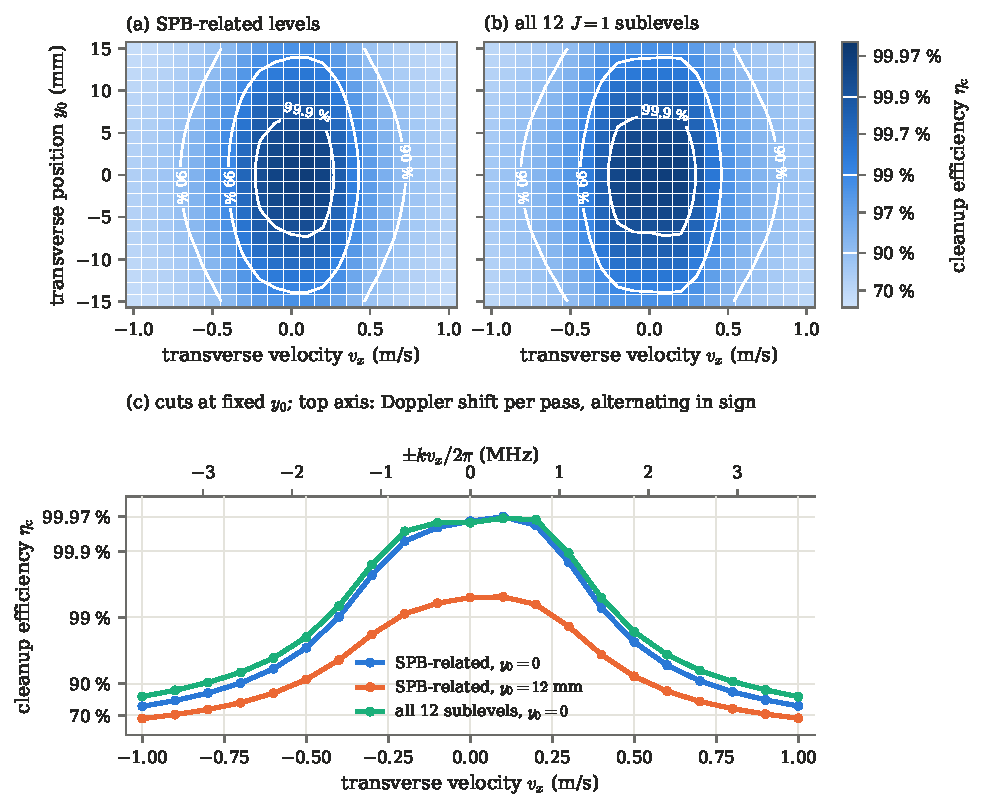
\includegraphics[width=\textwidth]{CU1_doppler_vx_y_map.pdf}
  \caption[CU1: cleanup versus transverse velocity and position]{CU1 cleanup versus transverse
  velocity $v_x$ and transverse position $y_0$ (\SI{80}{mW}, $+\SI{20.2}{MHz}$, \SI{4.8}{cm}
  beam, no EOM). (a) SPB-related initial state, (b) uniform 12-level initial state; logarithmic
  colour scale, white contours at 90, 99 and \SI{99.9}{\percent}; the grid was computed for
  $y_0\geq0$ and mirrored. (c) Cuts at fixed $y_0$; the top axis gives the Doppler shift per
  pass, whose sign alternates from pass to pass.}
  \label{fig:j1_doppler}
\end{figure}

\section{Average over the transverse distribution and choice of detuning}
\label{sec:j1_avg}

To compare settings by one number, the grids are averaged over an assumed transverse
distribution: $v_x$ Gaussian with \SI{1.8}{m/s} FWHM ($\sigma=\SI{0.76}{m/s}$), truncated at
$|v_x|\leq\SI{1}{m/s}$ because only these molecules reach the detection region (the cut keeps
\SI{81}{\percent} of the full Gaussian), and $y_0$ uniform within $|y_0|\leq\SI{15}{mm}$, the
coverage of the cylindrical lens~\cite{CleanupTheory2024}. The averages are trapezoidal sums on
the grid; the stored grids can be re-weighted with any other distribution. For the
comparison of settings a coarser grid was used ($v_x$ in steps of \SI{0.2}{m/s}, $y_0$ in
steps of \SI{3}{mm}); on the two full maps it agrees with the fine grid to \SI{0.1}{\percent}
(93.04 against \SI{93.1}{\percent}, 96.06 against \SI{96.15}{\percent}).

Table~\ref{tab:j1_avg} lists the results. At the on-axis optimum, $+\SI{20.2}{MHz}$, the
average is only \SI{95.5}{\percent} on the axis in $y_0$ and \SI{93.0}{\percent} over the full
distribution. Averaged over $v_x$, the cleanup without EOM has two maxima as a function of
detuning (Fig.~\ref{fig:j1_eom}a, row $\beta=0$), at $+\SI{19.0}{MHz}$ (\SI{97.4}{\percent}) and at
$+22.0$ to $+\SI{22.5}{MHz}$ (\SI{97.0}{}--\SI{97.2}{\percent}), on either side of the on-axis
optimum, where the average has a minimum. Over the full distribution $+\SI{19.0}{MHz}$ is the
better of the two, \SI{95.2}{\percent} against \SI{94.8}{\percent}. At these detunings the
cleanup on the axis at $v_x=0$ is worse (\SI{96.4}{\percent} at $+\SI{19.0}{MHz}$), but the
molecules with $|v_x|=0.4$--\SI{0.6}{m/s}, which are more numerous, are cleaned to
\SI{99.3}{}--\SI{99.8}{\percent} instead of \SI{94}{}--\SI{99.3}{\percent}
(Fig.~\ref{fig:j1_eom}b).

The distribution above was a first assumption. It has since been replaced by the result of a
beam simulation and by the acceptance of the detection laser (Sec.~\ref{sec:j1_present}):
$v_x$ Gaussian with $\sigma=\SI{0.65}{m/s}$, $y_0$ Gaussian with $\sigma=\SI{10.95}{mm}$,
counted only within $|v_x|\leq\SI{1}{m/s}$ and $|y_0|\leq\SI{8.5}{mm}$. The last column of
Table~\ref{tab:j1_avg} re-weights the same grids with it. The averages rise by 1 to
\SI{2.5}{\percent}, but the ranking is unchanged: $+\SI{19.0}{MHz}$ remains the best detuning
without EOM, and the EOM gains a further \SI{0.8}{\percent}.

\begin{table}[htbp]
  \centering
  \caption[CU1: cleanup averaged over the transverse distribution]{CU1: cleanup efficiency
  on the axis ($v_x=0$, $y_0=0$), averaged over $v_x$ at $y_0=0$, and averaged over $v_x$ and
  $y_0$ with the first assumed distribution (Gaussian $v_x$, \SI{1.8}{m/s} FWHM,
  $|v_x|\leq\SI{1}{m/s}$; $y_0$ uniform in $|y_0|\leq\SI{15}{mm}$). Last column: the same grids
  averaged with the beam-simulation distribution within the detection acceptance
  (Sec.~\ref{sec:j1_present}). \SI{80}{mW}, \SI{4.8}{cm} beam, SPB-related initial state;
  coarse grid. The adopted set point is in bold.}
  \label{tab:j1_avg}
  \small
  \setlength{\tabcolsep}{4pt}
  \begin{tabular}{lcccc}
    \toprule
    & & & \multicolumn{2}{c}{$v_x$- and $y_0$-averaged} \\
    \cmidrule(lr){4-5}
    setting & on axis & $v_x$-av., $y_0=0$ & first assumption & beam sim., acceptance \\
    \midrule
    no EOM, $+\SI{20.2}{MHz}$ & \SI{99.965}{\percent} & \SI{95.50}{\percent} & \SI{93.04}{\percent} & \SI{95.46}{\percent} \\
    \textbf{no EOM, $+\SI{19.0}{MHz}$} & \SI{96.36}{\percent} & \SI{97.44}{\percent} & \textbf{\SI{95.16}{\percent}} & \textbf{\SI{97.08}{\percent}} \\
    no EOM, $+\SI{22.0}{MHz}$ & \SI{98.70}{\percent} & \SI{96.97}{\percent} & \SI{94.83}{\percent} & \SI{96.83}{\percent} \\
    no EOM, $+\SI{22.5}{MHz}$ & \SI{95.48}{\percent} & \SI{97.18}{\percent} & \SI{94.72}{\percent} & \SI{96.73}{\percent} \\
    \midrule
    EOM $\beta=1.0$, $+\SI{19.0}{MHz}$ & \SI{98.49}{\percent} & \SI{98.12}{\percent} & \SI{95.87}{\percent} & \SI{97.73}{\percent} \\
    EOM $\beta=1.25$, $+\SI{19.5}{MHz}$ & \SI{99.41}{\percent} & \SI{98.15}{\percent} & \SI{96.00}{\percent} & \SI{97.85}{\percent} \\
    EOM $\beta=1.5$, $+\SI{20.0}{MHz}$ & \SI{99.45}{\percent} & \SI{98.17}{\percent} & \SI{96.06}{\percent} & \SI{97.89}{\percent} \\
    EOM $\beta=1.75$, $+\SI{20.0}{MHz}$ & \SI{99.03}{\percent} & \SI{98.23}{\percent} & \SI{96.03}{\percent} & \SI{97.87}{\percent} \\
    EOM $\beta=2.0$, $+\SI{20.2}{MHz}$ & \SI{97.91}{\percent} & \SI{98.11}{\percent} & \SI{95.76}{\percent} & \SI{97.66}{\percent} \\
    \bottomrule
  \end{tabular}
\end{table}

\section{A broadening EOM for CU1}
\label{sec:j1_eom}

Because the Doppler shift alternates in sign, it cannot be compensated by the laser frequency,
only covered by a broader laser spectrum. A phase EOM at \SI{1.6}{MHz}, available in the
laboratory, was tested for this purpose (Sec.~\ref{sec:laser}). Its sideband spacing is close
to $\Gamma/2\pi$, so the modulated spectrum is nearly continuous, with a width of about
$2(\beta+1)\times\SI{1.6}{MHz}$, \SI{8}{MHz} at $\beta=1.5$. The modulation depth was scanned
from 0 to 4 in steps of 0.5, with 1.25 and 1.75 added near the optimum, against the detuning
from $+16$ to $+\SI{23.5}{MHz}$ (part of the plane only, Fig.~\ref{fig:j1_eom}a), each point
averaged over $v_x$ at $y_0=0$; the best settings were then averaged over $y_0$ as well
(script \code{scripts/cu1\_eom\_doppler\_scan.py}, checkpoints in \code{tmp/cu1\_eom\_doppler/}).
With $\beta=0$ the modulated model reproduces the unmodulated one exactly.

\begin{itemize}
  \item The $v_x$-averaged cleanup has a broad maximum of \SI{98.1}{}--\SI{98.2}{\percent}
        for $\beta=1$--2 near $+\SI{20}{MHz}$ (best grid point $\beta=1.75$, $+\SI{20.0}{MHz}$,
        \SI{98.23}{\percent}). Beyond $\beta\approx2$ the power is spread too thinly; at
        $\beta=4$ the average drops to about \SI{92}{\percent}.
  \item Over the full distribution the best setting is $\beta=1.5$ at $+\SI{20.0}{MHz}$,
        \SI{96.06}{\percent} (\SI{96.15}{\percent} on the full map, run
        \code{doppler\_cu1\_spb\_eom1p6MHz\_beta1p5\_det20MHz}). The flat-topped velocity response
        (Fig.~\ref{fig:j1_eom}b) costs some efficiency on the axis (\SI{99.45}{\percent}) but
        keeps \SI{98.2}{}--\SI{99.0}{\percent} at $|v_x|=0.4$--\SI{0.6}{m/s}.
  \item The gain over the best setting without EOM is \SI{0.9}{\percent}
        (\SI{95.16}{\percent} to \SI{96.06}{\percent}), i.e.\ the remaining population falls
        from 4.8 to \SI{3.9}{\percent}. What is left is limited by the beam edges in $y_0$ and
        by the tails $|v_x|\geq\SI{0.8}{m/s}$, which need more power rather than more
        bandwidth.
  \item In the model the EOM and the polarization switching start with a fixed relative phase.
        In the experiment they are not synchronised; the effect of the relative phase has not
        been checked.
\end{itemize}

Because the gain is small, the EOM is not adopted for now. \textbf{The CU1 set point is
$+\SI{19.0}{MHz}$ without EOM}, which gives \SI{95.2}{\percent} over the assumed distribution,
against \SI{93.0}{\percent} at the on-axis optimum.

\begin{figure}[htbp]
  \centering
  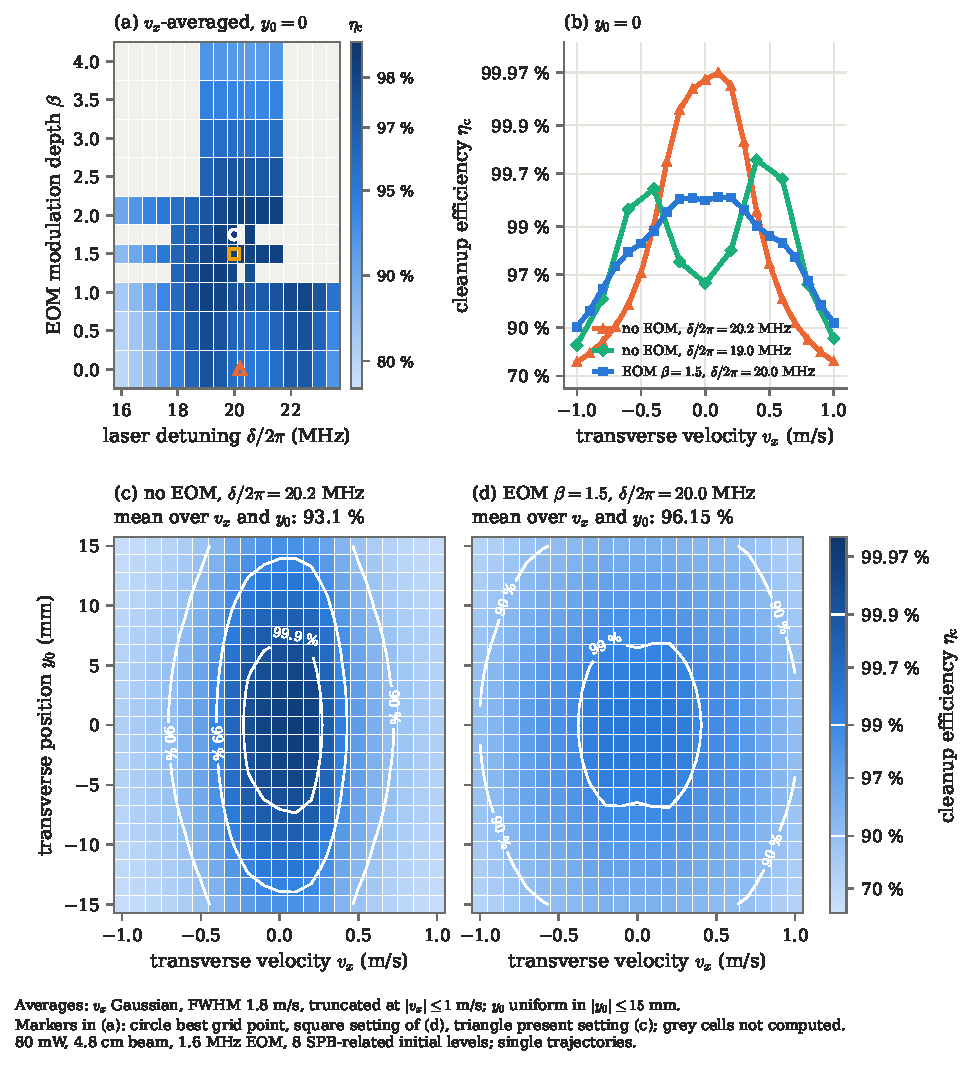
\includegraphics[width=\textwidth]{CU1_eom_doppler.pdf}
  \caption[CU1: broadening EOM against the Doppler shift]{CU1 with a \SI{1.6}{MHz} phase EOM.
  (a) Cleanup averaged over $v_x$ at $y_0=0$ versus modulation depth and detuning; grey cells
  were not computed. (b) Cleanup versus $v_x$ at $y_0=0$ at the on-axis optimum, at the set
  point chosen without EOM and at the best EOM setting. (c), (d) Maps over $v_x$ and $y_0$
  without and with the EOM, as in Fig.~\ref{fig:j1_doppler}, with the average over the
  distribution. SPB-related initial state, \SI{80}{mW}, \SI{4.8}{cm} beam.}
  \label{fig:j1_eom}
\end{figure}

\section{Trajectory at the set point}
\label{sec:j1_traj19}

Figure~\ref{fig:j1_traj19} shows a trajectory on the axis ($v_x=0$, $y_0=0$) at
$+\SI{19.0}{MHz}$, computed once for each of the 12 starting sublevels (script
\code{scripts/cu1\_trajectories.py}, populations every \SI{0.1}{\micro\second}, trace constant to
$2\times10^{-14}$). From the SPB-related start \SI{3.6}{\percent} remains in $J=1$, against
\SI{0.035}{\percent} at $+\SI{20.2}{MHz}$; from the uniform start \SI{2.5}{\percent}. Each
molecule scatters 1.49 photons (1.55 at $+\SI{20.2}{MHz}$). The removed molecules go to $J=3$
(\SI{47.5}{\percent}) and $J=2$ (\SI{46.2}{\percent}), with \SI{2.6}{\percent} in $J=4$ and
$7\times10^{-5}$ in $J=0$.

Almost all of the remaining population is in two levels:
$|F_1=\tfrac32,F=2,m_F=\pm2\rangle$ and $|F_1=\tfrac12,F=0,m_F=0\rangle$, of which 9.4 and
\SI{9.0}{\percent} remain when the molecule starts there. Every other sublevel keeps
\SI{0.22}{}--\SI{0.27}{\percent}. The reason is the ground-state structure in the field. The
12 sublevels form two groups \SI{2.4}{MHz} apart: the eight SPB-related levels, mainly
$|m_J|=1$, lie lower, and the four mainly $m_J=0$ levels, which include the main ground state,
lie higher. The transitions from the lower group to the excited $|m_F'|=1$ components are
about \SI{2.3}{MHz} higher in laser frequency ($+20.7$ to $+\SI{20.9}{MHz}$ against
$+\SI{18.5}{MHz}$). At $+\SI{19.0}{MHz}$ the laser is \SI{0.5}{MHz} from these components for
the upper group but 1.7--\SI{1.9}{MHz} for the lower group. The two levels left behind are in
the lower group and couple only weakly to the $|m_F'|=1$ components: $|M|^2=0.005$ for
$m_F=\pm2$ (X polarization) and 0.003 for $F=0$, which is reached only through its $F=2$
admixture, against 0.014 to 0.106 for the other levels of the group (X or Z polarization;
relative units). With Z polarization the stretched levels reach only $m_F'=\pm2$, whose
resonance lies \SI{17}{MHz} below the laser. A Doppler shift of about \SI{1.9}{MHz}
($|v_x|\approx\SI{0.5}{m/s}$) brings the lower group into resonance in half of the passes,
which is why this detuning works better for the velocity distribution than on the axis.

\begin{figure}[htbp]
  \centering
  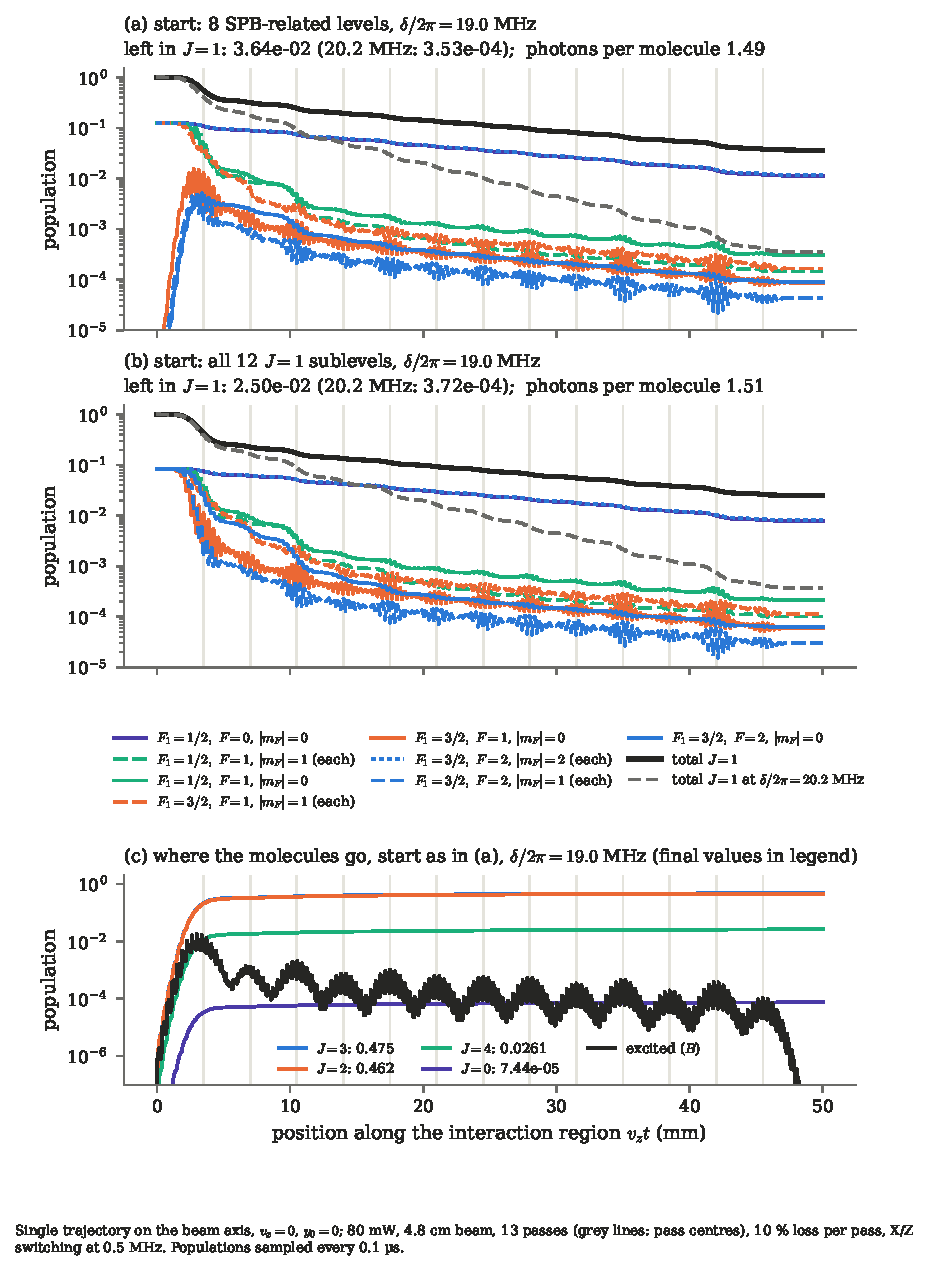
\includegraphics[width=\textwidth]{CU1_19MHz_J1_sublevels.pdf}
  \caption[CU1: sublevel populations at the set point]{CU1 at the set point $+\SI{19.0}{MHz}$
  on the axis ($v_x=0$, $y_0=0$), \SI{80}{mW}, no EOM. (a) $J=1$ sublevel populations from the
  SPB-related start (one curve per $\pm m_F$ pair, equal by symmetry), with the total and, for
  comparison, the total at $+\SI{20.2}{MHz}$. (b) The same from the uniform 12-level start. (c)
  Populations of the other rotational levels and of the excited state, start as in (a). Grey
  lines: pass centres.}
  \label{fig:j1_traj19}
\end{figure}

\section{CU1 at the present beam height and beam distribution}
\label{sec:j1_present}

\paragraph{Present conditions.} Three inputs have changed since the results above.
\begin{itemize}
  \item \textbf{Beam height.} In the experiment both cleanup beams are now about \SI{3}{cm}
        high ($\sigy=\SI{7.5}{mm}$). At the same \SI{80}{mW} the peak intensity is 1.6 times
        that of the \SI{4.8}{cm} beam; the model scales the power normalisation with the height
        (\code{build\_cu1(sigma\_y\_m=7.5e-3)}).
  \item \textbf{Beam distribution.} A simulation of the molecular beam with the electrostatic
        lens at \SI{25}{kV} gives, at CU1 (lens + \SI{0.5}{m}), Gaussian transverse positions with
        $\sigma_x\approx\sigma_y=\SI{10.95}{mm}$, and transverse velocities with
        $\sigma_{v_x}\approx\sigma_{v_y}=\SI{0.65}{m/s}$ (\SI{1.53}{m/s} FWHM), the same at
        both cleanup stages. The two transverse directions are equivalent, so $\sigma_{v_x}$ is
        used for the Doppler shift and $\sigma_y$ for the position along the beam height.
  \item \textbf{Detection acceptance.} The detection laser is \SI{2}{cm} wide ($x$) and
        \SI{1.7}{cm} high ($y$). Molecules outside it are not detected, so their cleanup does not
        matter. The average is therefore taken over $|y_0|\leq\SI{8.5}{mm}$, and over
        $|v_x|\leq\SI{1}{m/s}$ as before.
\end{itemize}
The \emph{mean in acceptance} is the average of the remaining population with Gaussian
weights in $v_x$ and $y_0$ inside this window. The logarithm of the remaining population is
interpolated linearly in $y_0$ between grid points, since \SI{8.5}{mm} falls between them; on the CU1 map
of Sec.~\ref{sec:j1_doppler}, halving the $y_0$ resolution changes the mean by
\SI{0.015}{\percent}. The cut is applied at the cleanup plane, i.e.\ the transverse drift
$v_y L/v$ between the cleanup and the detection region is neglected. For a path length of
\SI{2}{m} it is about \SI{7}{mm} r.m.s., comparable with the cut, so the population that is
eventually detected is not exactly the truncated Gaussian at the cleanup plane; the
distribution of the detected molecules at the cleanup planes, taken from the beam simulation,
would remove this approximation.

\paragraph{Choice of detuning.} With the higher intensity the detuning was scanned again
from $+17$ to $+\SI{23}{MHz}$ in steps of \SI{0.5}{MHz}, each point averaged over $v_x$
($\SI{0.2}{m/s}$ steps) and $y_0$ (0, 3, 6, \SI{9}{mm}), SPB-related start, no EOM (script
\code{scripts/cu1\_3cm\_scan.py}, 572 trajectories, about \SI{12}{min}). Table~\ref{tab:j1_3cm}
gives the result. The on-axis optimum moves to $+\SI{20.5}{MHz}$ (\SI{99.999}{\percent}), but
the mean in acceptance is again best at $+\SI{19.0}{MHz}$ (\SI{98.66}{\percent}); a parabola
through the three best points puts the maximum at $+\SI{19.1}{MHz}$, only \SI{0.05}{\percent}
higher. A second maximum lies at $+\SI{22.5}{MHz}$ (\SI{98.43}{\percent}). \textbf{The set point
$+\SI{19.0}{MHz}$ is kept.}

\begin{table}[htbp]
  \centering
  \caption[CU1 at \SI{3}{cm}: cleanup versus detuning]{CU1 with the \SI{3}{cm} beam
  (\SI{80}{mW}, no EOM, SPB-related start): cleanup on the axis, averaged over $v_x$ at
  $y_0=0$, and mean in the detection acceptance ($|v_x|\leq\SI{1}{m/s}$, $|y_0|\leq\SI{8.5}{mm}$,
  beam-simulation weights). The set point is in bold.}
  \label{tab:j1_3cm}
  \small
  \begin{tabular}{cccc}
    \toprule
    $\delta/2\pi$ (MHz) & on axis & $v_x$-averaged, $y_0=0$ & mean in acceptance \\
    \midrule
    17.0 & \SI{87.06}{\percent} & \SI{92.52}{\percent} & \SI{90.05}{\percent} \\
    17.5 & \SI{90.27}{\percent} & \SI{95.22}{\percent} & \SI{93.28}{\percent} \\
    18.0 & \SI{93.61}{\percent} & \SI{97.41}{\percent} & \SI{95.99}{\percent} \\
    18.5 & \SI{96.83}{\percent} & \SI{98.83}{\percent} & \SI{97.88}{\percent} \\
    \textbf{19.0} & \SI{99.01}{\percent} & \SI{99.34}{\percent} & \textbf{\SI{98.66}{\percent}} \\
    19.5 & \SI{99.85}{\percent} & \SI{99.12}{\percent} & \SI{98.44}{\percent} \\
    20.0 & \SI{99.994}{\percent} & \SI{98.58}{\percent} & \SI{97.71}{\percent} \\
    20.5 & \SI{99.999}{\percent} & \SI{98.10}{\percent} & \SI{97.07}{\percent} \\
    21.0 & \SI{99.988}{\percent} & \SI{98.03}{\percent} & \SI{97.01}{\percent} \\
    21.5 & \SI{99.938}{\percent} & \SI{98.42}{\percent} & \SI{97.58}{\percent} \\
    22.0 & \SI{99.73}{\percent} & \SI{98.96}{\percent} & \SI{98.29}{\percent} \\
    22.5 & \SI{98.75}{\percent} & \SI{99.18}{\percent} & \SI{98.43}{\percent} \\
    23.0 & \SI{96.16}{\percent} & \SI{98.54}{\percent} & \SI{97.37}{\percent} \\
    \bottomrule
  \end{tabular}
\end{table}

\paragraph{Map at the set point.} The full map at $+\SI{19.0}{MHz}$ ($v_x$ in steps of
\SI{0.1}{m/s}, $y_0$ in steps of \SI{1.5}{mm}, run \code{doppler\_cu1\_spb\_3cm\_det19MHz}) is
shown in Fig.~\ref{fig:j1_present}. On the axis the cleanup is \SI{99.01}{\percent}; the mean in
acceptance is \textbf{\SI{98.70}{\percent}}, against \SI{97.08}{\percent} for the \SI{4.8}{cm}
beam with the same weights (Table~\ref{tab:j1_avg}). The narrower beam helps because inside
the acceptance the higher intensity counts more than the loss of coverage at large $|y_0|$.
Along $y_0=0$ the cleanup is
\begin{center}
  \small
  \begin{tabular}{lccccccc}
    \toprule
    $|v_x|$ (m/s) & 0 & 0.2 & 0.3 & 0.4 & 0.5 & 0.7 & 1.0 \\
    \midrule
    $\etac$ at $v_x=-|v_x|$ (\%) & 99.01 & 99.52 & 99.85 & 99.97 & 99.98 & 99.67 & 93.4 \\
    $\etac$ at $v_x=+|v_x|$ (\%) & 99.01 & 99.66 & 99.92 & 99.99 & 99.99 & 99.83 & 94.7 \\
    \bottomrule
  \end{tabular}
\end{center}
so the best molecules are not those at rest but those at $|v_x|\approx\SI{0.5}{m/s}$.

\paragraph{Why $v_x=0$ is not the best.} The explanation follows from the two groups of ground
sublevels of Sec.~\ref{sec:j1_traj19}.
\begin{enumerate}
  \item In the field the 12 sublevels of $J=1$ form two groups \SI{2.4}{MHz} apart. The four
        mainly-$m_J=0$ levels, which include the main ground state, reach the driven
        $|m_F'|=1$ components at $\delta/2\pi\approx+\SI{18.5}{MHz}$; the eight SPB-related,
        mainly-$|m_J|=1$ levels only at $+20.7$ to $+\SI{20.9}{MHz}$. The latter group contains
        the two most weakly coupled levels, $|F_1=\tfrac32,F=2,m_F=\pm2\rangle$ and
        $|F_1=\tfrac12,F=0\rangle$ ($|M|^2=0.005$ and 0.003), which limit the cleanup whenever
        the laser is off their resonance.
  \item At $+\SI{19.0}{MHz}$ and $v_x=0$ the laser is \SI{0.5}{MHz} from the upper group but
        1.7--\SI{1.9}{MHz} below the SPB-related group in all 13 passes. The two weak levels are
        then pumped slowly, and \SI{1}{\percent} of the SPB-related population remains.
  \item A molecule with velocity $v_x$ sees the laser at $\delta+k_Lv_x$ in one half of the
        passes and at $\delta-k_Lv_x$ in the other (Sec.~\ref{sec:doppler}). At
        $|v_x|=\SI{0.5}{m/s}$, $k_Lv_x/2\pi=\SI{1.84}{MHz}$, so in half of the passes the laser
        appears at $+\SI{20.84}{MHz}$, on resonance with the SPB-related group, and the weak
        levels are emptied. This is where the map has its two maxima.
  \item The detuning that is best on the axis, $+\SI{20.5}{MHz}$, lies within \SI{0.4}{MHz} of
        the SPB-related group for $v_x=0$. For a moving molecule the Doppler shift then moves
        both halves of the passes away from that resonance, and without phase modulation the
        window is narrow: the mean in acceptance is only \SI{97.1}{\percent}. With $\sigma_{v_x}=\SI{0.65}{m/s}$ only
        \SI{30}{\percent} of the molecules have $|v_x|<\SI{0.25}{m/s}$, while \SI{58}{\percent}
        lie between 0.25 and \SI{1}{m/s}. Placing the laser so that the Doppler-shifted passes
        are resonant, at the cost of the molecules near rest, is therefore better on average.
  \item With the \SI{3}{cm} beam the loss at $v_x=0$ is small (\SI{99.0}{\percent}, against
        \SI{96.4}{\percent} with the \SI{4.8}{cm} beam), because the higher intensity
        power-broadens the transitions and partly bridges the \SI{1.8}{MHz} gap.
\end{enumerate}

\begin{figure}[htbp]
  \centering
  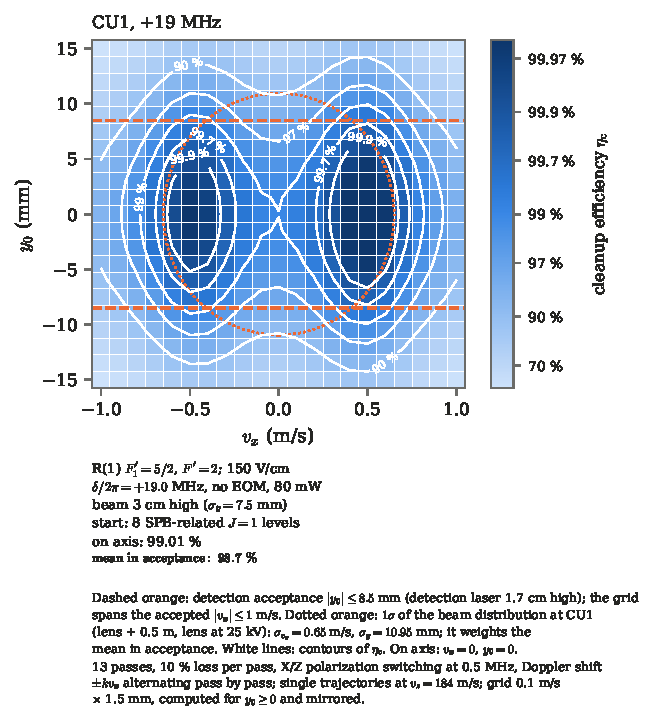
\includegraphics[width=0.62\textwidth]{cleanup_map_vx_y_CU1_current.pdf}
  \caption[CU1 at the present conditions: cleanup versus $v_x$ and $y_0$]{CU1 at the present
  conditions: cleanup efficiency versus transverse velocity and position at $+\SI{19.0}{MHz}$,
  \SI{80}{mW}, \SI{3}{cm} beam, no EOM, SPB-related start (run
  \code{doppler\_cu1\_spb\_3cm\_det19MHz}). Dashed lines: detection acceptance
  $|y_0|\leq\SI{8.5}{mm}$; dotted ellipse: $1\sigma$ of the beam distribution at CU1. The
  conditions and the mean in acceptance are given under the map.}
  \label{fig:j1_present}
\end{figure}

% =====================================================================
\chapter{CU2 results at \SI{200}{V/cm}}
\label{ch:j2}

\section{Operating field}

CU2 in the experiment now runs at about \SI{200}{V/cm}, and this field is used for all CU2
simulations from here on. Earlier simulations at \SI{250}{V/cm} are collected in
Appendix~\ref{app:legacy}. They are not combined with \SI{200}{V/cm} results, because the
detuning axes refer to field-dependent main resonances (Sec.~\ref{sec:couplings}) and because
$\Dmain$ changes from 219.93 to \SI{211.83}{MHz} (Eq.~\eqref{eq:dmain}). At \SI{200}{V/cm}
one-shot state identification is within its validated range and the build issues no ambiguity
warning.

\section{Configuration}

Baseline of Table~\ref{tab:baseline}, 56-level model (Appendix~\ref{app:code}):
\begin{itemize}
  \item beam~0 on R(2) $F_1'=7/2$, $F'=3$, $P_0=\SI{80}{mW}$; beam~1 on R(2) $F_1'=7/2$,
        $F'=4$, $P_1=\SI{24}{mW}$;
  \item common phase modulation, \SI{17.5}{MHz}, $\beta=1.5$;
  \item X/Z switching at \SI{0.5}{MHz} in antiphase;
  \item common multipass, \SI{10}{\percent} loss per pass, beam height \SI{2.4}{cm};
  \item frequency difference of the beams $\fAOM=200\pm\SI{15}{MHz}$, i.e.\
        $-26.83\leq(\delta_1-\delta_0)/2\pi\leq+\SI{3.17}{MHz}$ (Table~\ref{tab:aom}).
\end{itemize}

\section{Single trajectory at the former set point}

At the detunings that were optimal at \SI{250}{V/cm}, $(\delta_0,\delta_1)/2\pi=(+18.5,
-\SI{6.5}{MHz})$, which at \SI{200}{V/cm} correspond to $\fAOM=\SI{186.83}{MHz}$, the cleanup is
only $\etac=\SI{92.87}{\percent}$, with $\Ngam=1.42$. In the \SI{250}{V/cm} scans the same
detunings ($\fAOM=\SI{194.93}{MHz}$ there) gave \SI{99.99}{\percent}.

\begin{figure}[htbp]
  \centering
  \figplaceholder{CU2_200V_single_trajectory.pdf}
  \caption[CU2 at \SI{200}{V/cm}: populations along the interaction region]{CU2 at
  \SI{200}{V/cm}, single trajectory: populations of the 20 $J=2$ sublevels versus
  distance at $(+18.5,-\SI{6.5}{MHz})$, for comparison with the optima in
  Fig.~\ref{fig:j2_opt_sub}.}
  \label{fig:j2_single}
\end{figure}

\section{Laser-frequency scan at fixed AOM frequency}

In a first scan both detunings were shifted by a common offset, keeping
$(\delta_1-\delta_0)/2\pi=-\SI{25}{MHz}$. This is a scan of the laser frequency at fixed
$\fAOM=\SI{186.83}{MHz}$ (Table~\ref{tab:j2_corr}, Fig.~\ref{fig:j2_corr}). The best point is
an offset of $-\SI{4}{MHz}$, $(\delta_0,\delta_1)/2\pi=(+14.5,-\SI{10.5}{MHz})$, with
$\etac=\SI{99.33}{\percent}$. The cleanup changes by several percent between neighbouring
points, so the \SI{2}{MHz} grid is too coarse. For comparison, the CU1 optimum is about
\SI{1.6}{MHz} wide at the \SI{99.5}{\percent} level.

\begin{table}[htbp]
  \centering
  \caption[CU2 at \SI{200}{V/cm}: laser-frequency scan at fixed AOM frequency]{CU2 at
  \SI{200}{V/cm}: cleanup efficiency versus a common offset of both detunings at fixed
  $\fAOM=\SI{186.83}{MHz}$, i.e.\ $(\delta_1-\delta_0)/2\pi=-\SI{25}{MHz}$ (run
  \code{correlated\_detuning\_shared\_offset\_200V}, rtol $10^{-6}$).}
  \label{tab:j2_corr}
  \small
  \begin{tabular}{rrrc}
    \toprule
    offset (MHz) & $\delta_0/2\pi$ (MHz) & $\delta_1/2\pi$ (MHz) & $\etac$ \\
    \midrule
    $-10$ & 8.5 & $-16.5$ & \SI{96.25}{\percent} \\
    $-8$ & 10.5 & $-14.5$ & \SI{95.88}{\percent} \\
    $-6$ & 12.5 & $-12.5$ & \SI{97.15}{\percent} \\
    $-4$ & 14.5 & $-10.5$ & \textbf{\SI{99.33}{\percent}} \\
    $-2$ & 16.5 & $-8.5$ & \SI{97.96}{\percent} \\
    $0$ & 18.5 & $-6.5$ & \SI{92.94}{\percent} \\
    $+2$ & 20.5 & $-4.5$ & \SI{91.06}{\percent} \\
    $+4$ & 22.5 & $-2.5$ & \SI{96.46}{\percent} \\
    $+6$ & 24.5 & $-0.5$ & \SI{97.24}{\percent} \\
    $+8$ & 26.5 & $1.5$ & \SI{96.14}{\percent} \\
    \bottomrule
  \end{tabular}
\end{table}

\begin{figure}[htbp]
  \centering
  \figplaceholder{CU2_200V_laser_frequency_scan.pdf}
  \caption[CU2: laser-frequency scan at 200 and \SI{250}{V/cm}]{CU2 cleanup versus the common
  detuning offset at \SI{200}{V/cm} ($\fAOM=\SI{186.83}{MHz}$, Table~\ref{tab:j2_corr}) and,
  for reference, at \SI{250}{V/cm} ($\fAOM=\SI{194.93}{MHz}$, Appendix~\ref{app:legacy}).
  Lower axis: $\delta_0$; upper axis: $\delta_1$.}
  \label{fig:j2_corr}
\end{figure}

\section{Why the \SI{250}{V/cm} set point does not carry over}

The field change moves the two manifolds relative to each other. $\Dmain$ decreases by
\SI{8.1}{MHz}, and the component positions within each manifold (Table~\ref{tab:spread}) move
as well. With the AOM frequency of the former optimum, \SI{194.93}{MHz}, the detuning
difference at \SI{200}{V/cm} would be $-\SI{16.9}{MHz}$ instead of $-\SI{25}{MHz}$. With the
former detuning difference, the AOM must be set to \SI{186.83}{MHz}. Neither choice
reproduces the former alignment of both beams with their manifolds, and a scan of the laser
frequency alone, at one AOM frequency, cannot find the new optimum. Laser frequency and AOM
frequency must be optimised together.

\section{Two-dimensional optimisation in laser and AOM frequency}
\label{sec:j2_2d}

The optimisation uses the experimental coordinates $(\delta_0,\fAOM)$, with $\delta_1$ from
Eq.~\eqref{eq:aom} and $\Dmain=\SI{211.829}{MHz}$ computed from the model. It was run in three
stages with \code{scripts/cu2\_laser\_aom\_scan.py} (Appendix~\ref{app:code}), using the scan
tolerances of Table~\ref{tab:solver}.
\begin{enumerate}
  \item \textbf{Coarse grid}, \SI{2}{MHz} steps: $\delta_0/2\pi=+5\ldots+\SI{23}{MHz}$ (about
        one EOM period around the earlier best point) $\times$ $\fAOM=185\ldots\SI{215}{MHz}$
        (the full AOM range), 160 points.
  \item \textbf{Fine grids}, \SI{0.5}{MHz} steps over $\pm\SI{2}{MHz}$ around the three best
        separated local maxima of the coarse grid, 219 further points.
  \item \textbf{Confirmation} of the three best points with rtol $10^{-7}$, atol $10^{-9}$.
\end{enumerate}

\subsection{Coarse grid}

The cleanup varies between \SI{86.1}{\percent} and \SI{99.79}{\percent} over the grid
(Fig.~\ref{fig:j2_map}). Only 15 of the 160 points exceed \SI{99}{\percent}, and 6 exceed
\SI{99.5}{\percent}. The best points lie in two groups at $\delta_0/2\pi\approx\num{11}$ to
\SI{13}{MHz}, one with $\delta_1/2\pi\approx+\SI{8}{MHz}$ ($\fAOM\approx\SI{208}{MHz}$) and one
with $\delta_1/2\pi\approx-\SI{10}{MHz}$ ($\fAOM\approx\SI{190}{MHz}$). The two groups are
separated by about one EOM period in $\delta_1$: the $F'=4$ beam reaches the same components with
its carrier or with an adjacent sideband. A third, weaker maximum lies at the edge of the
$\delta_0$ range, near $\delta_0/2\pi=\SI{23}{MHz}$, $\fAOM=\SI{197}{MHz}$. At
$\fAOM=\SI{187}{MHz}$, next to the line of the earlier laser-frequency scan, the best grid value
is \SI{99.48}{\percent} at $\delta_0/2\pi=\SI{15}{MHz}$, consistent with the \SI{99.33}{\percent}
found there at $(14.5,\SI{186.83}{MHz})$. The earlier optimum is therefore only a side maximum.

\subsection{Fine grids and optimum}

Table~\ref{tab:j2_fine} summarises the three fine grids. The overall optimum lies in region~2:
\begin{equation}
  \frac{\delta_0}{2\pi}=+\SI{11.5}{MHz},\qquad \fAOM=\SI{191.0}{MHz}\quad
  \Bigl(\frac{\delta_1}{2\pi}=-\SI{9.33}{MHz}\Bigr),\qquad \etac=\SI{99.85}{\percent}.
\end{equation}
Region~1 gives almost the same cleanup, \SI{99.80}{\percent}, at
$(+\SI{11.5}{MHz},\SI{208.5}{MHz})$, $\delta_1/2\pi=+\SI{8.17}{MHz}$. Both points lie well
inside the AOM range. Compared with the first laser-frequency scan at fixed AOM frequency, the
remaining population falls from \SI{0.67}{\percent} to \SI{0.15}{\percent}.

\begin{table}[htbp]
  \centering
  \caption[CU2 at \SI{200}{V/cm}: fine grids]{CU2 at \SI{200}{V/cm}: best point of each
  \SI{0.5}{MHz} fine grid (runs \code{laser\_AOM\_2D\_200V\_fine\_0p5MHz\_region1--3}).}
  \label{tab:j2_fine}
  \small
  \begin{tabular}{lccccc}
    \toprule
    region & coarse maximum & best $\delta_0/2\pi$ & best $\fAOM$ & $\delta_1/2\pi$ & $\etac$ \\
    \midrule
    1 & $(11, 209)$\,MHz, \SI{99.79}{\percent} & \SI{11.5}{MHz} & \SI{208.5}{MHz} & $+\SI{8.17}{MHz}$ & \SI{99.80}{\percent} \\
    2 & $(11, 191)$\,MHz, \SI{99.77}{\percent} & \SI{11.5}{MHz} & \SI{191.0}{MHz} & $-\SI{9.33}{MHz}$ & \textbf{\SI{99.85}{\percent}} \\
    3 & $(23, 197)$\,MHz, \SI{99.55}{\percent} & \SI{23.5}{MHz} & \SI{196.5}{MHz} & $+\SI{8.17}{MHz}$ & \SI{99.56}{\percent} \\
    \bottomrule
  \end{tabular}
\end{table}

\subsection{Confirmation with tighter tolerances}

The three best points, all in region~2, were recomputed with rtol $10^{-7}$
(Table~\ref{tab:j2_confirm}). The cleanup changes by \num{3e-5} at most, so the scan
tolerance is adequate at the optimum.

\begin{table}[htbp]
  \centering
  \caption[CU2 at \SI{200}{V/cm}: confirmation of the best points]{CU2 at \SI{200}{V/cm}:
  best points recomputed with rtol $10^{-7}$, atol $10^{-9}$ (run
  \code{laser\_AOM\_2D\_200V\_confirm\_rtol1e-7}).}
  \label{tab:j2_confirm}
  \small
  \begin{tabular}{cccc}
    \toprule
    $\delta_0/2\pi$ & $\fAOM$ & $\etac$, rtol $10^{-6}$ & $\etac$, rtol $10^{-7}$ \\
    \midrule
    \SI{11.5}{MHz} & \SI{191.0}{MHz} & \SI{99.8535}{\percent} & \SI{99.8508}{\percent} \\
    \SI{11.0}{MHz} & \SI{191.5}{MHz} & \SI{99.8352}{\percent} & \SI{99.8319}{\percent} \\
    \SI{12.0}{MHz} & \SI{190.5}{MHz} & \SI{99.8301}{\percent} & \SI{99.8275}{\percent} \\
    \bottomrule
  \end{tabular}
\end{table}

\subsection{Width of the optimum}

Table~\ref{tab:j2_window} gives the ranges over which the cleanup stays above a given level,
along the laser frequency at fixed AOM frequency and along the AOM frequency at fixed laser
frequency. A shift along the laser frequency is also what a common shift of both lines
produces, for example from a change of the electric field. Both optima are 0.5--\SI{1.5}{MHz}
wide at the \SI{99.7}{\percent} level and 2--\SI{3}{MHz} wide at \SI{99}{\percent}.
Region~2 has the higher peak, and region~1 is somewhat wider, in particular along the AOM
frequency. The design-study estimate of a \SI{2}{MHz} line shift from the field variation
across the cleanup region (Fig.~\ref{fig:efield}) is comparable to the \SI{99}{\percent} width,
so the field uniformity at \SI{200}{V/cm} should be checked.

The fine grids also show that both optima are elongated along lines of constant $\delta_1$,
$\delta_0+2\pi\fAOM=\text{const}$ (Fig.~\ref{fig:j2_fine}). Along such a line, i.e.\ with the
$F'=4$ detuning held fixed, the cleanup in region~2 stays above \SI{99.6}{\percent} for
$\delta_0/2\pi$ from 10.0 to \SI{13.0}{MHz}. Moving across it, a change of $\delta_0$ by
\SI{0.5}{MHz} combined with a change of $\delta_1$ by \SI{1}{MHz} already lowers the cleanup to
\SI{99.4}{\percent}. The efficiency is therefore set mainly by the detuning of the $F'=4$ beam:
$\delta_1$ must be held to about $\pm\SI{0.5}{MHz}$, while $\delta_0$ tolerates about
$\pm\SI{1.5}{MHz}$ if $\delta_1$ is kept fixed. Since a drift of the laser frequency shifts both
detunings together, the laser frequency is limited by the tighter $\delta_1$ tolerance.

\begin{table}[htbp]
  \centering
  \caption[CU2 at \SI{200}{V/cm}: width of the optima]{CU2 at \SI{200}{V/cm}: ranges (on the
  \SI{0.5}{MHz} grid) within which the cleanup exceeds the given level, through the best point
  of regions~1 and~2.}
  \label{tab:j2_window}
  \small
  \begin{tabular}{llccc}
    \toprule
    region & direction & $>\SI{99.7}{\percent}$ & $>\SI{99.5}{\percent}$ & $>\SI{99}{\percent}$ \\
    \midrule
    2 & $\delta_0/2\pi$ at $\fAOM=\SI{191.0}{MHz}$ & 11.0--\SI{12.0}{MHz} & 11.0--\SI{12.0}{MHz} & 10.5--\SI{12.5}{MHz} \\
    2 & $\fAOM$ at $\delta_0/2\pi=\SI{11.5}{MHz}$ & 190.5--\SI{191.5}{MHz} & 190.0--\SI{191.5}{MHz} & 189.5--\SI{192.0}{MHz} \\
    1 & $\delta_0/2\pi$ at $\fAOM=\SI{208.5}{MHz}$ & 11.5--\SI{12.0}{MHz} & 11.0--\SI{12.5}{MHz} & 10.5--\SI{13.0}{MHz} \\
    1 & $\fAOM$ at $\delta_0/2\pi=\SI{11.5}{MHz}$ & 208.0--\SI{209.5}{MHz} & 208.0--\SI{210.0}{MHz} & 207.5--\SI{210.5}{MHz} \\
    \bottomrule
  \end{tabular}
\end{table}

\begin{figure}[htbp]
  \centering
  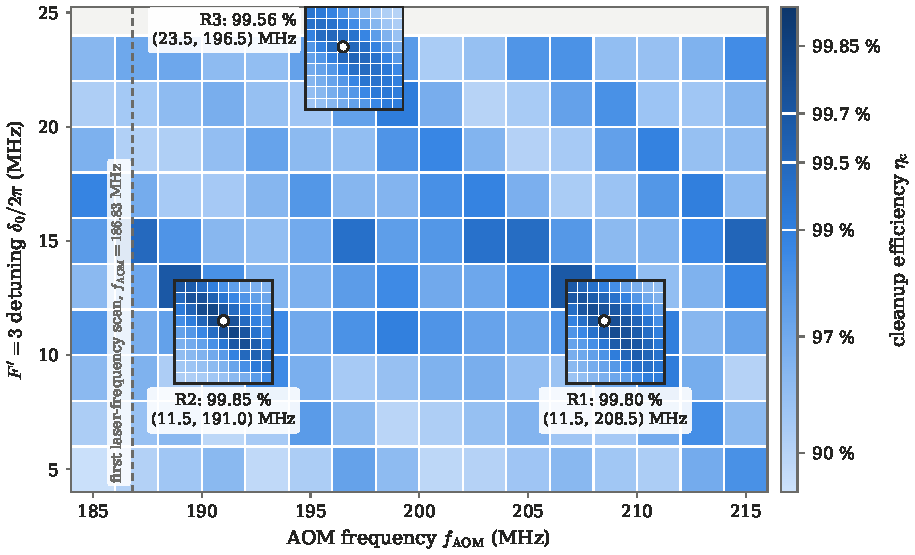
\includegraphics[width=\textwidth]{CU2_200V_laser_AOM_map.pdf}
  \caption[CU2 at \SI{200}{V/cm}: cleanup versus laser and AOM frequency]{CU2 cleanup
  efficiency at \SI{200}{V/cm} versus the AOM frequency $\fAOM$ (full range
  185--\SI{215}{MHz}) and the $F'=3$ detuning $\delta_0$, i.e.\ the laser frequency. Colour:
  remaining $J=2$ population on a logarithmic scale, labelled in cleanup efficiency; darker is
  better; white lines on the colour bar mark 99, 99.5 and \SI{99.7}{\percent}. Large cells: coarse
  \SI{2}{MHz} grid (run \code{laser\_AOM\_2D\_200V\_coarse\_2MHz}); outlined boxes: \SI{0.5}{MHz}
  fine grids R1--R3, with their best points (circles). Dashed: the line
  $\fAOM=\SI{186.83}{MHz}$ of the first laser-frequency scan. The grey band above
  $\delta_0/2\pi=\SI{24}{MHz}$ was not computed outside R3.}
  \label{fig:j2_map}
\end{figure}

\begin{figure}[htbp]
  \centering
  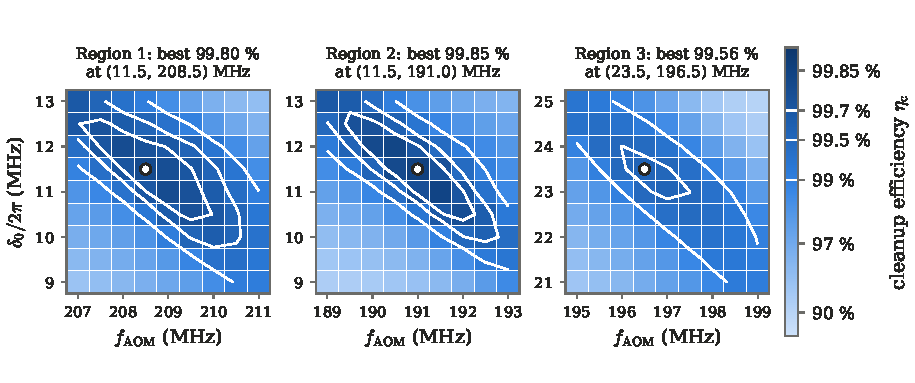
\includegraphics[width=\textwidth]{CU2_200V_fine_regions.pdf}
  \caption[CU2 at \SI{200}{V/cm}: fine grids around the optima]{CU2 at \SI{200}{V/cm}:
  \SI{0.5}{MHz} fine grids R1--R3 (runs \code{laser\_AOM\_2D\_200V\_fine\_0p5MHz\_region1--3}),
  same colour scale as Fig.~\ref{fig:j2_map}. White contours: 99, 99.5 and
  \SI{99.7}{\percent}; circles: best points. The high-efficiency areas run along lines of
  constant $\delta_1$ (slope $-1$).}
  \label{fig:j2_fine}
\end{figure}

\subsection{Trajectories at the two optima}
\label{sec:j2_traj}

Single trajectories at the best points of R1 and R2 were computed with rtol $10^{-7}$, saving
the populations every \SI{0.1}{\micro\second}. The photon number was taken from the solver's
running integral (\code{output="photon\_integral"}) rather than from the sampled excited
population. The script is \code{scripts/cu2\_optimum\_trajectories.py}.
Figures~\ref{fig:j2_opt_pop} and~\ref{fig:j2_opt_sub} show the result, and
Table~\ref{tab:j2_opt} lists the final populations.

\begin{itemize}
  \item \textbf{Pass by pass.} The first pass removes about \SI{75}{\percent} of the $J=2$
        population. Each later pass multiplies what is left by 0.5 to 0.8, following the
        alternating powers of the multipass passes: strong passes remove more. The population
        still falls at the last pass, so more passes or more power would improve the cleanup
        further.
  \item \textbf{Destination.} The removed molecules end almost entirely in $J=3$ (53--54\,\%) and
        $J=4$ (44--45\,\%), with \SI{1.7}{\percent} in $J=5$ and $3\times10^{-5}$ in $J=1$. The
        excited-state population peaks at \SI{1.4}{\percent} in the first pass. Each molecule
        scatters 1.5 photons on average.
  \item \textbf{Bottleneck.} The remaining population is dominated by the stretched sublevels
        $|F_1=\tfrac52,F=3,m_F=\pm3\rangle$: \SI{74}{\percent} of it in R1 and \SI{56}{\percent}
        in R2. Next come the $F_1=\tfrac32$, $F=2$ sublevels, \SI{18}{\percent} in R1 and
        \SI{35}{\percent} in R2. R2 cleans the stretched sublevels better, which is why its
        total is lower.
  \item \textbf{Tolerance check.} With rtol $10^{-7}$ the R1 optimum gives \SI{99.823}{\percent},
        against \SI{99.803}{\percent} in the scan; the R2 value, \SI{99.851}{\percent}, agrees with
        Table~\ref{tab:j2_confirm}.
\end{itemize}

\begin{table}[htbp]
  \centering
  \caption[CU2 at \SI{200}{V/cm}: final populations at the two optima]{CU2 at \SI{200}{V/cm}:
  final populations at the two optima (rtol $10^{-7}$), and the photon number per molecule from
  the running integral.}
  \label{tab:j2_opt}
  \small
  \begin{tabular}{lcc}
    \toprule
    & R1 & R2 \\
    \midrule
    $(\delta_0/2\pi,\ \fAOM,\ \delta_1/2\pi)$ (MHz) & $(11.5,\ 208.5,\ +8.17)$ & $(11.5,\ 191.0,\ -9.33)$ \\
    cleanup efficiency $\etac$ & \SI{99.823}{\percent} & \textbf{\SI{99.851}{\percent}} \\
    remaining in $J=2$ & $1.77\times10^{-3}$ & $1.49\times10^{-3}$ \\
    \quad of which $F_1=\tfrac52$, $F=3$, $m_F=\pm3$ & \SI{74}{\percent} & \SI{56}{\percent} \\
    \quad of which $F_1=\tfrac32$, $F=2$ & \SI{18}{\percent} & \SI{35}{\percent} \\
    $J=3$ & 0.541 & 0.529 \\
    $J=4$ & 0.439 & 0.452 \\
    $J=5$ & 0.0177 & 0.0173 \\
    $J=1$ & $3.2\times10^{-5}$ & $3.3\times10^{-5}$ \\
    photons per molecule $\Ngam$ & 1.50 & 1.51 \\
    \bottomrule
  \end{tabular}
\end{table}

\begin{figure}[htbp]
  \centering
  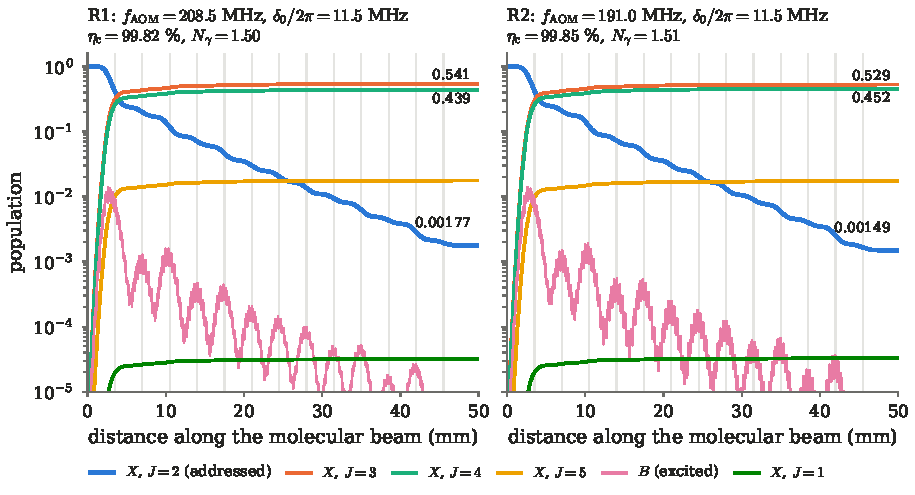
\includegraphics[width=\textwidth]{CU2_200V_optimum_populations.pdf}
  \caption[CU2 at \SI{200}{V/cm}: rotational-level populations at the two optima]{CU2 at
  \SI{200}{V/cm}: populations of the rotational levels along the interaction region at the
  optima of R1 ($\delta_1/2\pi=+\SI{8.17}{MHz}$) and R2 ($\delta_1/2\pi=-\SI{9.33}{MHz}$),
  logarithmic scale. Grey vertical lines: centres of the 13 passes. The excited-state population
  oscillates with the \SI{0.5}{MHz} polarization switching and the \SI{17.5}{MHz} phase
  modulation; it is sampled every \SI{0.1}{\micro\second}.}
  \label{fig:j2_opt_pop}
\end{figure}

\begin{figure}[htbp]
  \centering
  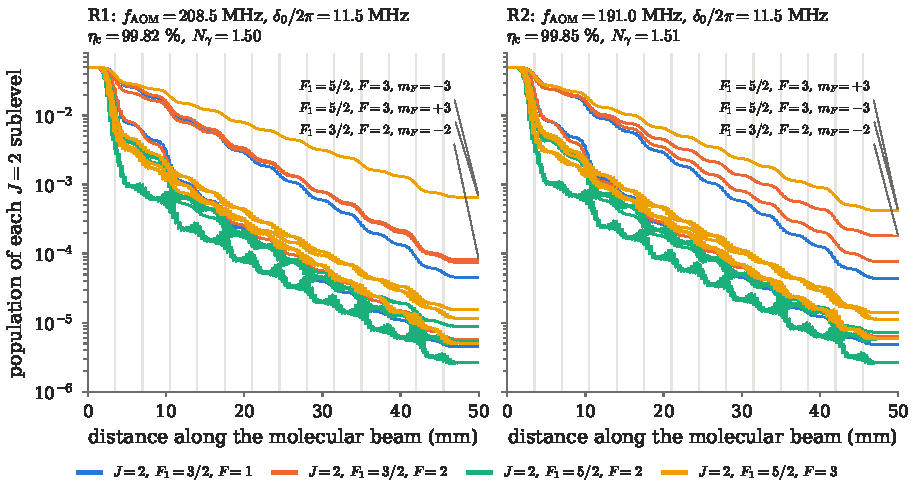
\includegraphics[width=\textwidth]{CU2_200V_optimum_J2_sublevels.pdf}
  \caption[CU2 at \SI{200}{V/cm}: $J=2$ sublevel populations at the two optima]{CU2 at
  \SI{200}{V/cm}: populations of the 20 $J=2$ sublevels at the optima of R1 and R2, coloured by
  hyperfine level $(F_1,F)$; the three sublevels with the most population left are labelled.
  In R1 the two stretched sublevels $m_F=\pm3$ end at the same value.}
  \label{fig:j2_opt_sub}
\end{figure}

\subsection{Why both AOM frequencies work}
\label{sec:j2_two_aom}

Figure~\ref{fig:j2_scheme} shows the excited sublevels addressed by the two beams at
\SI{200}{V/cm}, together with the carrier and sidebands of each beam at the two optima. Its
frequency axis is measured from the $F'=3$ main resonance, so the $F'=4$ sublevels and the
beam-1 lines appear \SI{211.83}{MHz} higher than on the $\delta_1$ axis used in the text and in
Table~\ref{tab:j2_comb}. Each sublevel is placed at the coupling-weighted mean of its
resonances from the 20 $J=2$ sublevels; the ground-state hyperfine structure spreads them by at
most \SI{1.5}{MHz}. Which sublevels the light actually drives is estimated with a weak-field
excitation rate. For sublevel $e$ this is
\begin{equation}
  R_e=\sum_{g\in J=2}\ \sum_{p}|M^{(p)}_{eg}|^2\sum_n J_n(\beta)^2\,
  \frac{1}{1+\bigl[2(\nu_{eg}-\nu_n)/(\Gamma/2\pi)\bigr]^2},
  \label{eq:rate}
\end{equation}
with $\nu_{eg}$ the resonance of the pair and $\nu_n$ the comb lines; saturation, the
polarization switching and coherent effects are not included. The explanation follows from three
observations.

\begin{enumerate}
  \item \textbf{The two settings differ by exactly one EOM period.} The AOM frequencies differ
        by $208.5-191.0=\SI{17.5}{MHz}$, the EOM frequency, while beam~0 is unchanged. The comb
        of beam~1, at $\delta_1/2\pi+n\times\SI{17.5}{MHz}$, therefore occupies the same
        frequencies in R1 and R2. Only the order $n$ of each line shifts by one: the line that is
        the carrier in R1 is the first-order sideband in R2, and so on (upper half of
        Fig.~\ref{fig:j2_scheme}).
  \item \textbf{Carrier and first-order sidebands carry almost the same power.} At $\beta=1.5$
        the carrier carries $J_0^2=\SI{26}{\percent}$ of the power and each first-order
        sideband $J_1^2=\SI{31}{\percent}$. The two lines that matter most sit on the strongest
        $F'=4$ components in both settings: the line at $+\SI{8.17}{MHz}$ on $m_F'=0$
        ($+\SI{8.65}{MHz}$, the most strongly coupled $F'=4$ sublevel), and the line at
        $-\SI{9.33}{MHz}$ on $m_F'=\pm2$ ($-\SI{10.32}{MHz}$). These two components are
        \SI{19.0}{MHz} apart, close to the comb spacing, so two adjacent lines can sit on both at
        once. Whether the carrier or a first-order sideband does the work changes the power on
        each by only about \SI{16}{\percent} (Table~\ref{tab:j2_comb}).
  \item \textbf{The outer lines decide which setting is slightly better.} By
        Eq.~\eqref{eq:rate}, beam~1 drives mainly $m_F'=0$ in both settings, and $m_F'=\pm2$ at
        \SI{35}{\percent} of that rate in R1 and \SI{25}{\percent} in R2. All other $F'=4$
        sublevels stay below \SI{4}{\percent}. The bottleneck of Table~\ref{tab:j2_opt}, the
        stretched ground sublevels $|F_1=\tfrac52,F=3,m_F=\pm3\rangle$, is hardly pumped by
        beam~0: its rate through $F'=3$ is 40 to 50 times lower than through $F'=4$. In $F'=4$ it
        couples mainly to $m_F'=\pm4$ ($-\SI{31.41}{MHz}$) and $m_F'=\pm3$
        ($-\SI{20.44}{MHz}$), which lie far from the two main lines. R2 has a first-order sideband
        (\SI{31}{\percent}) at $-\SI{26.83}{MHz}$, \SI{4.6}{MHz} from the strongly coupled
        $m_F'=\pm4$; R1 has only a second-order sideband there (\SI{5}{\percent}). The
        stretched sublevels are therefore pumped \SI{15}{\percent} faster in R2. R1 in turn has
        \SI{31}{\percent} instead of \SI{26}{\percent} on $m_F'=\pm2$, and pumps the
        $F_1=\tfrac32$, $F=2$ sublevels \SI{11}{\percent} faster. Both trends agree with the
        composition of the remaining population: the stretched sublevels are \SI{56}{\percent} of
        it in R2 against \SI{74}{\percent} in R1, and $F_1=\tfrac32$, $F=2$ is \SI{35}{\percent}
        against \SI{18}{\percent}. Since the stretched sublevels are the main bottleneck, R2 ends
        with less population left, \SI{99.85}{\percent} against \SI{99.82}{\percent}.
\end{enumerate}

Because the comb repeats every \SI{17.5}{MHz}, the optimum repeats every \SI{17.5}{MHz} in
$\fAOM$. Within the AOM range only these two copies exist: the next ones, at 173.5 and
\SI{226}{MHz}, lie outside 185--\SI{215}{MHz}. Beam~0 is the same in both settings. Its
first-order sideband sits on the $F'=3$, $m_F'=\pm1$ components ($+\SI{28.41}{MHz}$), and its
carrier lies \SI{3}{MHz} below the $m_F'=\pm2$ components.

\begin{table}[htbp]
  \centering
  \caption[CU2: beam-1 comb lines and $F'=4$ sublevels at the two optima]{CU2 at
  \SI{200}{V/cm}: comb lines of beam~1 near the $F'=4$ sublevels, with their order $n$ and power
  fraction $J_n(1.5)^2$ in R1 and R2. Positions on the $\delta_1$ axis.}
  \label{tab:j2_comb}
  \small
  \begin{tabular}{rlcc}
    \toprule
    line (MHz) & nearest $F'=4$ sublevel(s) & R1: $n$, power & R2: $n$, power \\
    \midrule
    $+8.17$ & $m_F'=0$, $P'=-$ at $+8.65$ (strongest) & $0$, \SI{26}{\percent} & $+1$, \SI{31}{\percent} \\
    $-9.33$ & $m_F'=\pm2$, $P'=-$ at $-10.32$ & $-1$, \SI{31}{\percent} & $0$, \SI{26}{\percent} \\
    $+25.67$ & $m_F'=\pm1$, $P'=+$ at $+22.50$ & $+1$, \SI{31}{\percent} & $+2$, \SI{5}{\percent} \\
    $-26.83$ & $m_F'=\pm3$ at $-20.83$, $\pm4$ at $-31.41$, $P'=-$ & $-2$, \SI{5}{\percent} & $-1$, \SI{31}{\percent} \\
    $+43.17$ & $m_F'=\pm3$, $P'=+$ at $+44.43$ & $+2$, \SI{5}{\percent} & $+3$, \SI{0.4}{\percent} \\
    \bottomrule
  \end{tabular}
\end{table}

\begin{figure}[htbp]
  \centering
  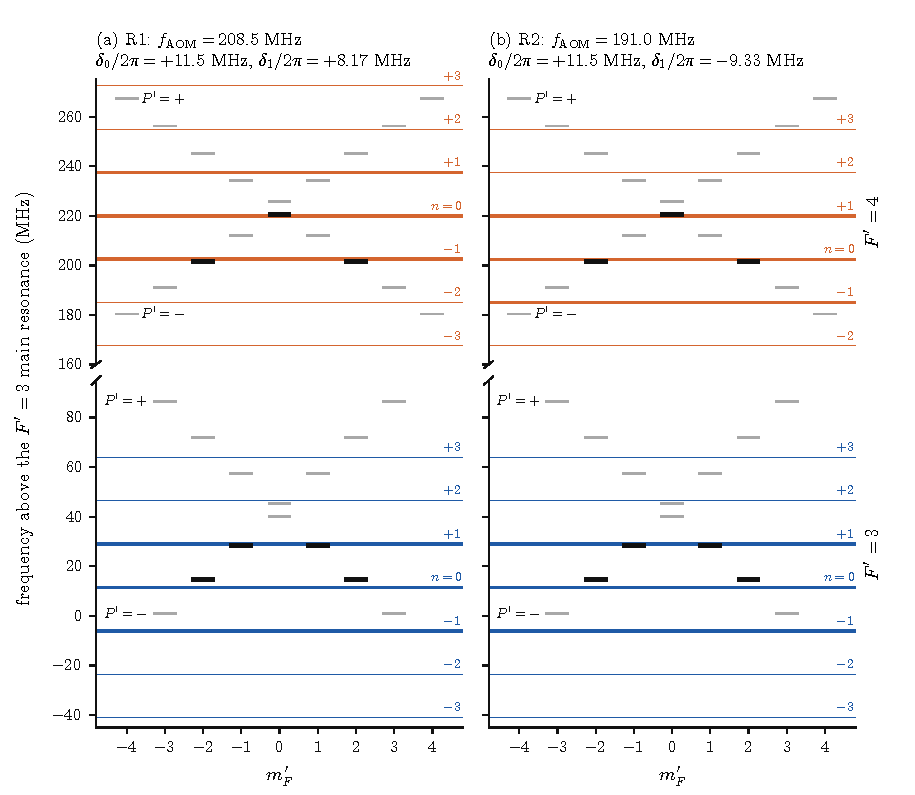
\includegraphics[width=\textwidth]{CU2_200V_level_diagram_R1_R2.pdf}
  \caption[CU2 at \SI{200}{V/cm}: level diagram with the laser combs of R1 and R2]{CU2 at
  \SI{200}{V/cm}: excited sublevels of $B$, $J'=3$, $F_1'=7/2$ addressed from $X$, $J=2$, and
  the laser combs at the optima of (a) R1 and (b) R2. The frequency axis is broken between
  $F'=3$ (bottom) and $F'=4$ (top) and gives the transition frequency above the $F'=3$ main
  resonance; the $F'=4$ main resonance lies at \SI{211.83}{MHz}. Each dash is one excited
  sublevel at the coupling-weighted mean of its resonances from the 20 $J=2$ sublevels (which
  span at most \SI{1.5}{MHz}). The two $\Lambda$-doublet components with the same $m_F'$ are
  aligned vertically and form the $P'=-$ and $P'=+$ branches. Sublevels driven by the light,
  with an excitation rate, Eq.~\eqref{eq:rate}, of at least \SI{5}{\percent} of the most strongly
  driven sublevel of the same beam, are shown in bold. Coloured lines: carrier ($n=0$) and
  phase-modulation sidebands $n$ of beam~0 (blue, $F'=3$) and beam~1 (orange, $F'=4$), with line
  width proportional to the power fraction $J_n(1.5)^2$ (0.26, 0.31, 0.05 and 0.004 for
  $|n|=0$--3). Beam~0 is the same in (a) and (b). The beam-1 lines lie at the same frequencies in
  both columns, and only their orders differ by one. Script: \code{scripts/cu2\_level\_scheme.py}.}
  \label{fig:j2_scheme}
\end{figure}

\section{Transverse velocity and position at the present beam height}
\label{sec:j2_doppler}

\paragraph{Setup.} The two optima were evaluated over the transverse velocity and position
under the present conditions of Sec.~\ref{sec:j1_present}: beam height \SI{3}{cm}
($\sigy=\SI{7.5}{mm}$) at the same 80 + \SI{24}{mW}, i.e.\ 0.8 times the peak intensity of the
\SI{2.4}{cm} beam used for the optimisation (\code{build(sigma\_y\_m=7.5e-3)}). The two beams run
through the same multipass in the same direction, so the Doppler shift, Eq.~\eqref{eq:doppler},
is common to both: in the $(\delta_0,\fAOM)$ plane it moves the operating point along the laser
frequency at fixed AOM frequency, in alternate directions in alternate passes. A coarse grid
was computed, $v_x$ from $-1$ to $+\SI{1}{m/s}$ in steps of \SI{0.2}{m/s} and $y_0$ from 0 to
\SI{15}{mm} in steps of \SI{3}{mm} (66 trajectories, about \SI{50}{min} per run), for R1 and R2
and for two initial states, all 20 $J=2$ sublevels and the four SPB source levels ($J=2$,
$m_J=0$, lens weights 2/3 for the singlet and 1/9 for each triplet level) (script
\code{scripts/cu2\_doppler\_scan.py}, runs \code{doppler\_cu2\_\{R1,R2\}\_\{uniform,spb\}\_3cm\_coarse}).
The means use the beam-simulation distribution at CU2 (lens + \SI{1.0}{m}): $\sigma_{v_x}=\SI{0.65}{m/s}$
and $\sigma_y=\SI{10.35}{mm}$, within the detection acceptance $|v_x|\leq\SI{1}{m/s}$,
$|y_0|\leq\SI{8.5}{mm}$.

\begin{table}[htbp]
  \centering
  \caption[CU2: cleanup over the transverse distribution]{CU2 at \SI{200}{V/cm} with the
  \SI{3}{cm} beam: cleanup on the axis, averaged over $v_x$ at $y_0=0$, and mean in the detection
  acceptance; for comparison, the mean with the $y_0$ range extended to \SI{15}{mm} (coarse
  grid, beam-simulation weights). The recommended setting is in bold.}
  \label{tab:j2_doppler}
  \small
  \setlength{\tabcolsep}{4pt}
  \begin{tabular}{llcccc}
    \toprule
    $\fAOM$ & start & on axis & $v_x$-av., $y_0=0$ & \textbf{in acceptance} & $|y_0|\leq\SI{15}{mm}$ \\
    \midrule
    R2, \SI{191.0}{MHz} & all 20 sublevels & \SI{99.59}{\percent} & \SI{97.72}{\percent} & \SI{96.10}{\percent} & \SI{91.84}{\percent} \\
    \textbf{R1}, \SI{208.5}{MHz} & all 20 sublevels & \SI{99.52}{\percent} & \SI{98.16}{\percent} & \textbf{\SI{96.66}{\percent}} & \SI{92.51}{\percent} \\
    R2, \SI{191.0}{MHz} & SPB source levels & \SI{99.975}{\percent} & \SI{99.67}{\percent} & \SI{99.35}{\percent} & \SI{98.42}{\percent} \\
    \textbf{R1}, \SI{208.5}{MHz} & SPB source levels & \SI{99.974}{\percent} & \SI{99.81}{\percent} & \textbf{\SI{99.57}{\percent}} & \SI{98.79}{\percent} \\
    \bottomrule
  \end{tabular}
\end{table}

\paragraph{Results.} Table~\ref{tab:j2_doppler} and Fig.~\ref{fig:j2_doppler} summarise the
four runs.
\begin{itemize}
  \item \textbf{The transverse position dominates.} With $\sigy=\SI{7.5}{mm}$ the intensity
        falls to 73, 49, 28 and \SI{14}{\percent} of its axial value at $y_0=6$, 9, 12 and
        \SI{15}{mm}. From the uniform start at $v_x=0$ the cleanup falls accordingly from
        \SI{99.5}{}--\SI{99.6}{\percent} on the axis to \SI{98.6}{\percent} at \SI{6}{mm},
        \SI{96.0}{\percent} at \SI{9}{mm} and \SI{88.7}{}--\SI{89.0}{\percent} at \SI{12}{mm}.
        The detection acceptance cuts this tail: over $|y_0|\leq\SI{15}{mm}$ the mean would be
        about \SI{4}{\percent} lower for the uniform start.
  \item \textbf{The transverse velocity matters much less than for CU1.} From the uniform start
        on the axis the cleanup is still \SI{97.8}{}--\SI{98.4}{\percent} at $|v_x|=\SI{0.4}{m/s}$
        and \SI{94.7}{}--\SI{95.5}{\percent} at \SI{1}{m/s}, against \SI{78}{\percent} at
        \SI{1}{m/s} for CU1 at its on-axis optimum (Table~\ref{tab:j1_vx}). Each CU2 beam carries
        a comb of five significant lines and the two beams address the 32 sublevels of $F'=3$ and
        $F'=4$ (both $\Lambda$-doublet components), so a
        shift of a few MHz detunes some lines from their components while others come closer,
        and the cleanup degrades gradually instead of leaving a narrow resonance.
  \item \textbf{R1 is more robust than R2.} On the axis R2 is marginally better, but over the
        distribution R1 wins for both starts (96.66 against \SI{96.10}{\percent}, 99.57 against
        \SI{99.35}{\percent}); its cleanup falls more slowly with $|v_x|$. With transverse motion
        included, \textbf{R1 ($\fAOM=\SI{208.5}{MHz}$) is the recommended CU2 setting.}
  \item \textbf{The SPB source levels are cleaned much better than the average sublevel}
        (\SI{99.6}{\percent} against \SI{96.7}{\percent} in acceptance), as on the axis
        (Sec.~\ref{sec:j2_traj}): they couple strongly to $F'=4$, while the uniform start
        contains the slowly pumped stretched levels, which dominate where the intensity is low.
        Which of the two numbers applies depends on how the $J=2$ population entering CU2 is
        divided between the molecules SPB did not transfer and the molecules that CU1 pumped
        into $J=2$.
  \item The lower peak intensity of the \SI{3}{cm} beam reduces the on-axis cleanup from the
        uniform start from \SI{99.85}{\percent} (\SI{2.4}{cm}) to \SI{99.59}{\percent} at R2. R1 and R2
        were optimised on the axis for the \SI{2.4}{cm} beam; a re-optimisation of
        $(\delta_0,\fAOM)$ for the \SI{3}{cm} beam and the transverse distribution has not been
        done.
\end{itemize}

\begin{figure}[htbp]
  \centering
  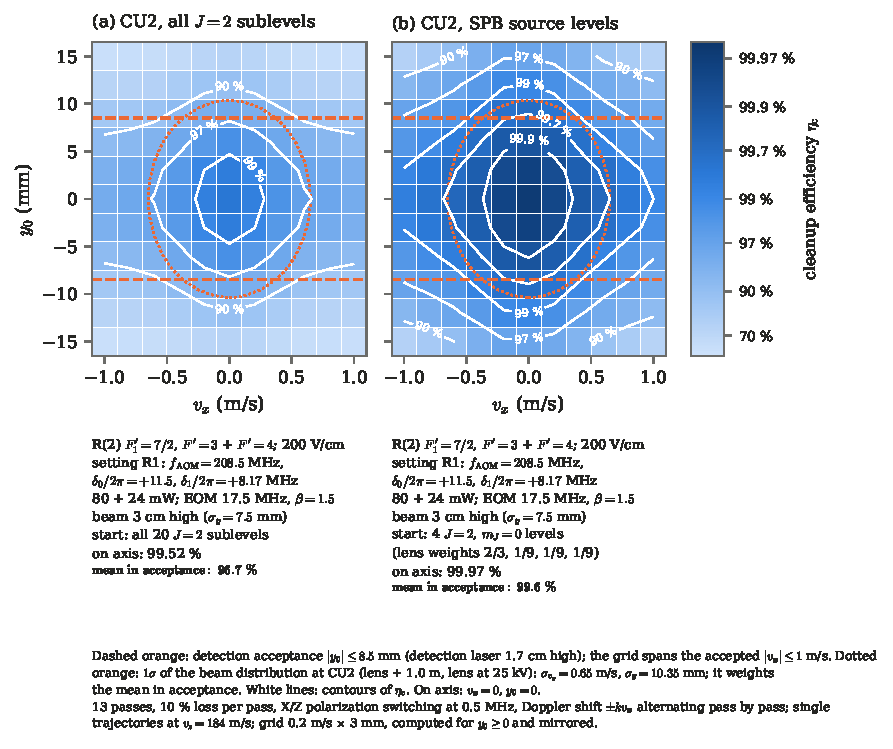
\includegraphics[width=0.9\textwidth]{cleanup_map_vx_y_CU2_current.pdf}
  \caption[CU2 at the present conditions: cleanup versus $v_x$ and $y_0$]{CU2 at the present
  conditions, setting R1 ($\fAOM=\SI{208.5}{MHz}$, $\delta_0/2\pi=+\SI{11.5}{MHz}$), \SI{3}{cm}
  beam, 80 + \SI{24}{mW}: cleanup versus transverse velocity and position from (a) all 20 $J=2$
  sublevels and (b) the four SPB source levels (coarse grid, mirrored in $y_0$). Dashed lines:
  detection acceptance; dotted ellipse: $1\sigma$ of the beam distribution at CU2. The conditions
  and the mean in acceptance are given under each map.}
  \label{fig:j2_doppler}
\end{figure}

% =====================================================================
\chapter{Numerical checks}
\label{ch:checks}

\begin{itemize}
  \item \textbf{Trace.} $\mathrm{Tr}\,\rho$ stays one to better than $10^{-14}$ in every
        model: no population leaves the modelled manifold.
  \item \textbf{Reproducibility.} The CU1 coarse and fine detuning scans, run separately,
        agree exactly at their four common points.
  \item \textbf{Tolerance.} At \SI{200}{V/cm} and $(+18.5,-\SI{6.5}{MHz})$, a point with much
        population left, the single trajectory with rtol $10^{-7}$ leaves 0.07125 in $J=2$ and
        the scan with rtol $10^{-6}$ leaves 0.07062, a difference of $6\times10^{-4}$. At the
        optimum of the two-dimensional scan the difference is only $3\times10^{-5}$
        (Table~\ref{tab:j2_confirm}), so the scan tolerance is adequate where it matters.
  \item \textbf{$\Lambda$-doublet partner.} Effect on the CU1 cleanup: $6\times10^{-6}$.
  \item \textbf{State identification.} No ambiguity warning at 150 and \SI{200}{V/cm}; one at
        \SI{250}{V/cm} (two states, margin 0.012).
  \item \textbf{Cross-coupling.} All neglected couplings between the two CU2 beams and the
        other excited level are detuned by more than \SI{50}{MHz} at every scanned point, the
        minimum being at $\delta_0/2\pi=\SI{5}{MHz}$, $\fAOM=\SI{185}{MHz}$, and by \SI{63}{MHz}
        at the optimum (Sec.~\ref{sec:couplings}).
\end{itemize}

Still to be done: convergence in $J_{\max}$ at \SI{200}{V/cm} for the eigenvectors (not only
the energies). Photon numbers from the running integral are available for the two CU2 optima
(Sec.~\ref{sec:j2_traj}); the other photon numbers in this report use the trapezoidal rule on
the \SI{1}{\micro\second} output grid.

% =====================================================================
\chapter{Conclusions and outlook}
\label{ch:conclusion}

\begin{table}[htbp]
  \centering
  \caption{Main results (baseline of Table~\ref{tab:baseline}).}
  \label{tab:summary}
  \small
  \begin{tabularx}{\textwidth}{Lr}
    \toprule
    quantity & value \\
    \midrule
    CU1: cleanup at \SI{80}{mW}, $+\SI{20.2}{MHz}$, \SI{150}{V/cm} & \SI{99.96}{\percent} \\
    CU1: detuning window for $\etac>\SI{99.9}{\percent}$ & \SI{0.6}{MHz} \\
    CU1: cleanup at \SI{110}{mW} (grid point $+\SI{20.8}{MHz}$) & \SI{99.955}{\percent} \\
    CU1: effect of the $\Lambda$-doublet partner & $6\times10^{-6}$ \\
    CU1: $|v_x|$ for $\etac>\SI{99.9}{\percent}$ / $>\SI{99}{\percent}$ (on axis, $+\SI{20.2}{MHz}$) & 0.2 / \SI{0.4}{m/s} \\
    CU1: average over $v_x$ (\SI{1.8}{m/s} FWHM) and $|y_0|\leq\SI{15}{mm}$, $+\SI{20.2}{MHz}$ & \SI{93.0}{\percent} \\
    CU1: same, at the set point $+\SI{19.0}{MHz}$ (no EOM) & \SI{95.2}{\percent} \\
    CU1: same, with a \SI{1.6}{MHz} EOM, $\beta=1.5$, $+\SI{20.0}{MHz}$ (not adopted) & \SI{96.1}{\percent} \\
    CU2: $F'=4$ minus $F'=3$ main resonance at 200 / \SI{250}{V/cm} & 211.83 / \SI{219.93}{MHz} \\
    CU2, \SI{200}{V/cm}: reachable $(\delta_1-\delta_0)/2\pi$ for $\fAOM=200\pm\SI{15}{MHz}$ & $-26.83$ to $+\SI{3.17}{MHz}$ \\
    CU2, \SI{200}{V/cm}: cleanup at the former detunings $(+18.5,-\SI{6.5}{MHz})$ & \SI{92.9}{\percent} \\
    CU2, \SI{200}{V/cm}: best at $\fAOM=\SI{186.83}{MHz}$ (laser-frequency scan) & \SI{99.33}{\percent} \\
    CU2, \SI{200}{V/cm}: optimum $\delta_0/2\pi=+\SI{11.5}{MHz}$, $\fAOM=\SI{191.0}{MHz}$ (rtol $10^{-7}$) & \SI{99.85}{\percent} \\
    CU2, \SI{200}{V/cm}: second optimum $\delta_0/2\pi=+\SI{11.5}{MHz}$, $\fAOM=\SI{208.5}{MHz}$ & \SI{99.80}{\percent} \\
    CU2, \SI{200}{V/cm}: width of the optimum at \SI{99}{\percent} (laser / AOM frequency) & 2 / \SI{2.5}{MHz} \\
    CU2 reference at \SI{250}{V/cm} (Appendix~\ref{app:legacy}) & \SI{99.991}{\percent} \\
    \midrule
    \multicolumn{2}{l}{\emph{present conditions: \SI{3}{cm} beams, beam simulation at \SI{25}{kV}, detection acceptance}} \\
    CU1, $+\SI{19.0}{MHz}$, no EOM: mean in acceptance / on axis & \SI{98.7}{\percent} / \SI{99.0}{\percent} \\
    CU1: on-axis optimum (\SI{3}{cm}) & $+\SI{20.5}{MHz}$, \SI{99.999}{\percent} \\
    CU2, R1 ($\fAOM=\SI{208.5}{MHz}$), all 20 sublevels: mean in acceptance / on axis & \SI{96.7}{\percent} / \SI{99.5}{\percent} \\
    CU2, R1, SPB source levels: mean in acceptance / on axis & \SI{99.6}{\percent} / \SI{99.97}{\percent} \\
    CU2, R2 ($\fAOM=\SI{191.0}{MHz}$), all 20 sublevels / SPB source levels & \SI{96.1}{\percent} / \SI{99.35}{\percent} \\
    \bottomrule
  \end{tabularx}
\end{table}

On the beam axis CU1 removes \SI{99.96}{\percent} of the $J=1$ population with a single
\SI{80}{mW} beam and no phase modulation, as the design study anticipated. The optimum is
narrow (\SI{0.6}{MHz} at the \SI{99.9}{\percent} level), and this makes CU1 sensitive to the
transverse velocity: in the multipass the Doppler shift alternates in sign from pass to pass, so
it cannot be compensated by the laser frequency, and the cleanup falls below \SI{99}{\percent}
for $|v_x|>\SI{0.4}{m/s}$. For an assumed Gaussian distribution of \SI{1.8}{m/s} FWHM (cut at
\SI{1}{m/s}) and a uniform transverse position within \SI{15}{mm}, the average is
\SI{93.0}{\percent} at the on-axis optimum and \SI{95.2}{\percent} at $+\SI{19.0}{MHz}$, which is
adopted as the set point. A \SI{1.6}{MHz} phase EOM gains another \SI{0.9}{\percent}
(\SI{96.1}{\percent}) and is not adopted for now. The remaining population is then limited by
the beam edges in $y_0$ and by the tails of the velocity distribution, i.e.\ by the power.

Under the present conditions, a \SI{3}{cm} beam, the transverse distribution of the beam
simulation and the acceptance of the detection laser, CU1 at $+\SI{19.0}{MHz}$ removes
\SI{98.7}{\percent} of the $J=1$ population that is eventually detected
(Sec.~\ref{sec:j1_present}); $+\SI{19.0}{MHz}$ remains the best detuning, although the on-axis
optimum has moved to $+\SI{20.5}{MHz}$. At this set point the molecules at rest are cleaned less
well (\SI{99.0}{\percent}) than those at $|v_x|\approx\SI{0.5}{m/s}$ (\SI{99.99}{\percent}): the
eight SPB-related sublevels lie \SI{2.4}{MHz} below the other four, and only a Doppler shift of
about \SI{1.8}{MHz} brings them into resonance, in half of the passes. Since most molecules move
transversely, this trade is favourable on average.

For CU2 the change of field from 250 to \SI{200}{V/cm} invalidates the former set point,
because the relative position of the $F'=3$ and $F'=4$ manifolds moves by \SI{8}{MHz}. Since
the two beams are coupled by the AOM, the new optimum had to be found in laser frequency and AOM
frequency together, within $\fAOM=200\pm\SI{15}{MHz}$. The two-dimensional optimisation finds
\SI{99.85}{\percent} at $\delta_0/2\pi=+\SI{11.5}{MHz}$, $\fAOM=\SI{191.0}{MHz}$, confirmed with
tighter tolerances, and a nearly equivalent optimum (\SI{99.80}{\percent}) at
$\fAOM=\SI{208.5}{MHz}$, exactly one EOM period higher in $\fAOM$. Both work because the
comb of the $F'=4$ beam then lies at the same frequencies, with the roles of carrier and
first-order sideband exchanged, and these carry almost the same power at $\beta=1.5$
(Sec.~\ref{sec:j2_two_aom}). The remaining $J=2$
population is \SI{0.15}{\percent}, against \SI{0.67}{\percent} for the best point of the first
laser-frequency scan. Both optima are 2--\SI{3}{MHz} wide at the \SI{99}{\percent} level.

With the present \SI{3}{cm} beam and the transverse distribution (Sec.~\ref{sec:j2_doppler}),
the second optimum, $\fAOM=\SI{208.5}{MHz}$, is the more robust one and is recommended: it removes
\SI{96.7}{\percent} of a uniformly populated $J=2$ level and \SI{99.6}{\percent} of the population
in the SPB source levels within the detection acceptance. For CU2 the transverse position matters
more than the transverse velocity: the comb of the two phase-modulated beams tolerates Doppler
shifts of a few MHz, but the intensity at the edge of the acceptance is only about
\SI{50}{\percent} of the axial value.

Next steps:
\begin{enumerate}[itemsep=0pt,topsep=2pt]
  \item Use the beam simulation to give the transverse distribution of the molecules that reach
        the detection laser, at the CU1 and CU2 planes. This removes the approximation of
        applying the detection cut at the cleanup planes; the stored grids only need to be
        re-weighted.
  \item CU2: re-optimise $(\delta_0,\fAOM)$ for the \SI{3}{cm} beam with the transverse average,
        starting from R1, and scan the power split between the two beams. The stretched
        sublevels $|F_1=\tfrac52,F=3,m_F=\pm3\rangle$, pumped almost only by the \SI{24}{mW}
        $F'=4$ beam, limit the cleanup at low intensity (Sec.~\ref{sec:j2_traj}).
  \item Sensitivity of the CU2 optimum to the electric field (e.g.\ 198 and \SI{202}{V/cm}), which
        requires rebuilding the model, and the field uniformity across the cleanup region at
        \SI{200}{V/cm}.
  \item Repeat the geometry scans at constant power (normalisation $\propto1/\sigy$); both
        builders now support it (\code{sigma\_y\_m}).
  \item Correct the stored metadata of the CU1 run \code{detuning\_withoutP-\_-20to\_100MHz},
        which records \code{retain\_opposite\_parity\_levels=True} although it was run with
        the 21-level model.
\end{enumerate}

% =====================================================================
\appendix

\chapter{Model parameters}
\label{app:params}

\begin{table}[!ht]
  \centering
  \caption{Parameters of the simulation.}
  \label{tab:params}
  \footnotesize
  \begin{tabularx}{\textwidth}{lLl}
    \toprule
    symbol & quantity & value \\
    \midrule
    \multicolumn{3}{l}{\emph{fields and molecule}} \\
    $E$ & electric field along $z$ & \SI{150}{V/cm} (CU1), \SI{200}{V/cm} (CU2) \\
    $B$ & magnetic field along $z$ & \SI{1e-3}{\gauss} \\
    $\Gamma$ & $B$-state decay rate & \SI{1.0101e7}{s^{-1}} ($\Gamma/2\pi=\SI{1.608}{MHz}$) \\
    $\Dxb$ & $X$--$B$ transition dipole moment & \SI{2.6675506e-30}{C\,m} \\
    $J_{\max}$ & rotational truncation of $X$ and $B$ & 4 (CU1), 5 (CU2) \\
    \midrule
    \multicolumn{3}{l}{\emph{trajectory}} \\
    $v$ & forward velocity & \SI{184}{m/s} \\
    $v_x$ & transverse velocity & $-1\ldots+\SI{1}{m/s}$ scanned \\
    $k_Lv_x/2\pi$ & Doppler shift, sign alternating per pass & \SI{3.68}{MHz} per m/s \\
    $y_0$ & transverse offset & $0\ldots\SI{15}{mm}$ scanned (mirrored) \\
    $\sigma_{v_x}$ & transverse velocity spread (beam sim., \SI{25}{kV}) & \SI{0.65}{m/s}, both stages \\
    $\sigma_y$ & beam size (beam sim., \SI{25}{kV}) & \SI{10.95}{mm} (CU1), \SI{10.35}{mm} (CU2) \\
    & detection acceptance & $|v_x|\leq\SI{1}{m/s}$, $|y_0|\leq\SI{8.5}{mm}$ \\
    & first assumption (Sec.~\ref{sec:j1_avg}) & $v_x$: \SI{1.8}{m/s} FWHM; $y_0$ uniform in \SI{15}{mm} \\
    $L_{\mathrm{IR}}$, $T$ & length and duration of the interaction region & \SI{5}{cm}, \SI{271.7}{\micro\second} \\
    \midrule
    \multicolumn{3}{l}{\emph{laser beam}} \\
    & number of passes & 13 \\
    $s_n$ & pass centres & $n\times\SI{3.5}{mm}$, $n=1\ldots13$ \\
    $L$ & loss per pass & \SI{10}{\percent} \\
    $\sigs$ & Gaussian width along the beam & \SI{0.75}{mm} (\SI{3}{mm} full $4\sigma$) \\
    $\sigy$ & Gaussian width transverse & \SI{12}{mm} (CU1, \SI{4.8}{cm}), \SI{6}{mm} (CU2, \SI{2.4}{cm}) \\
    & present beam height, both stages & \SI{3}{cm} ($\sigy=\SI{7.5}{mm}$), constant power \\
    $\wpol/2\pi$ & polarization switching frequency & \SI{0.5}{MHz}, square wave, X/Z \\
    \midrule
    \multicolumn{3}{l}{\emph{CU1}} \\
    & transition & R(1) $F_1'=5/2$, $F'=2$ \\
    $P$ & laser power & \SI{80}{mW} (scans 10--\SI{110}{mW}) \\
    $\delta/2\pi$ & detuning: set point / on-axis optimum & $+\SI{19.0}{MHz}$ / $+\SI{20.2}{MHz}$ \\
    & optional phase EOM (not adopted) & \SI{1.6}{MHz}; best $\beta=1.5$ at $+\SI{20.0}{MHz}$ \\
    $m$ & main-pair matrix element & 0.1004 \\
    \midrule
    \multicolumn{3}{l}{\emph{CU2}} \\
    & transitions & R(2) $F_1'=7/2$, $F'=3$ and $F'=4$ \\
    $P_0$, $P_1$ & beam powers & \SI{80}{mW}, \SI{24}{mW} \\
    $\wmod/2\pi$, $\beta$ & phase modulation, common to both beams & \SI{17.5}{MHz}, 1.5 \\
    $\fAOM$ & AOM frequency (beam separation) & $200\pm\SI{15}{MHz}$ \\
    $\Dmain$ & separation of the main resonances & \SI{211.83}{MHz} (\SI{200}{V/cm}) \\
    $\delta_0/2\pi$, $\fAOM$ & optimum (laser, AOM) & $+\SI{11.5}{MHz}$, \SI{191.0}{MHz} ($\delta_1/2\pi=-\SI{9.33}{MHz}$) \\
    $m_0$, $m_1$ & main-pair matrix elements & 0.0948, 0.2286 \\
    \midrule
    \multicolumn{3}{l}{\emph{integration}} \\
    & method & \code{dopri5}, Rust, \code{expanded\_sparse}, \code{decomposed} \\
    & initial step, tolerances & \SI{2}{ns}; rtol $10^{-7}$, atol $10^{-9}$ (CU2 scans: $10^{-6}$, $10^{-8}$) \\
    \bottomrule
  \end{tabularx}
\end{table}

\chapter{Reference results at \SI{250}{V/cm}}
\label{app:legacy}

These CU2 results were obtained before the operating field was changed to \SI{200}{V/cm}.
They use the same 56-level two-transition model and the same baseline beam parameters, and are
kept as a reference only.

\begin{itemize}
  \item Laser-frequency scan at fixed $\fAOM=\SI{194.93}{MHz}$
        ($(\delta_1-\delta_0)/2\pi=-\SI{25}{MHz}$), combined from three runs covering
        $\delta_0/2\pi=-58.5$ to $+\SI{141.5}{MHz}$ in \SI{1}{MHz} steps (one gap, 100.5 to
        \SI{102.5}{MHz}): best $\etac=\SI{99.991}{\percent}$ at $(+18.5,-\SI{6.5}{MHz})$
        (Fig.~\ref{fig:legacy}). Along this direction the cleanup falls to
        \SI{99.94}{\percent} at $-\SI{1}{MHz}$ and \SI{99.83}{\percent} at $+\SI{1}{MHz}$ from the
        optimum, and to \SI{99.03}{\percent} and \SI{98.68}{\percent} at $\mp\SI{2}{MHz}$.
  \item $3\times3$ grid around this point (Table~\ref{tab:legacy_grid}).
\end{itemize}

\begin{table}[htbp]
  \centering
  \caption[CU2 at \SI{250}{V/cm}: $3\times3$ detuning grid]{CU2 at \SI{250}{V/cm}: cleanup
  efficiency (\%) on a $3\times3$ grid (run \code{Fprime3\_Fprime4\_detuning}).}
  \label{tab:legacy_grid}
  \small
  \begin{tabular}{lccc}
    \toprule
    & $\delta_1/2\pi=-\SI{7.5}{MHz}$ & $-\SI{6.5}{MHz}$ & $-\SI{5.5}{MHz}$ \\
    \midrule
    $\delta_0/2\pi=+\SI{17.5}{MHz}$ & 99.944 & 99.870 & 99.519 \\
    $\delta_0/2\pi=+\SI{18.5}{MHz}$ & 99.984 & \textbf{99.991} & 99.958 \\
    $\delta_0/2\pi=+\SI{19.5}{MHz}$ & 99.801 & 99.918 & 99.833 \\
    \bottomrule
  \end{tabular}
\end{table}

\begin{figure}[htbp]
  \centering
  \figplaceholder{CU2_250V_laser_frequency_scan_combined.pdf}
  \caption[CU2 at \SI{250}{V/cm}: combined laser-frequency scan]{CU2 at \SI{250}{V/cm}:
  cleanup versus $\delta_0$ at fixed $\fAOM=\SI{194.93}{MHz}$ (run
  \code{correlated\_detuning\_shared\_offset\_boarder\_combined}). Reference only.}
  \label{fig:legacy}
\end{figure}

\paragraph{Single-transition variant.} A variant with only R(2) $F'=3$, in which one laser is
split by an AOM into two phase-modulated tones (\SI{80}{\percent} and \SI{20}{\percent} of
\SI{100}{mW}) offset by $\Delta_{\mathrm{AOM}}$, was simulated at \SI{250}{V/cm} with a
38-level model. At $\delta/2\pi=\Delta_{\mathrm{AOM}}/2\pi=\SI{18.5}{MHz}$ it reaches
$\etac=\SI{99.05}{\percent}$ with $\Ngam=1.53$, with the removed molecules in $J=3$
(\SI{59.9}{\percent}), $J=4$ (\SI{37.2}{\percent}) and $J=5$ (\SI{1.9}{\percent}). It
corresponds to step~2 of the design (Sec.~\ref{sec:design_cu2}), which the design study found
limited by dark states, and is not pursued further.

\chapter{Code and data}
\label{app:code}

\begin{table}[htbp]
  \centering
  \caption{Notebooks and scripts.}
  \label{tab:code}
  \small
  \begin{tabularx}{\textwidth}{lL}
    \toprule
    file & contents \\
    \midrule
    \code{SPB\_cleanup\_J1-J2F2.ipynb} & CU1: build, single trajectory, detuning,
      power and geometry scans, HDF5 readback, optimum and re-run \\
    \code{SPB\_cleanup\_J2\_J3F4\_opposite\_parity.ipynb} & CU2 two-transition scheme:
      build, single trajectory, detuning scans, combination of runs \\
    \code{SPB\_cleanup\_J2\_J3F3\_2laser.ipynb} & CU2 single-transition variant
      (\SI{250}{V/cm}; not pursued) \\
    \code{scripts/scan\_progress.py} & chunked grid scan with progress bar
      (\code{grid\_scan\_with\_progress}) \\
    \code{scripts/scan\_hdf.py} & HDF5 storage with metadata (\code{save\_scan\_hdf},
      \code{load\_scan\_hdf}) \\
    \code{scripts/migrate\_j2\_j3f4\_notebook.py} & one-off migration of the CU2 notebook
      from the Julia workflow \\
    \code{scripts/refactor\_scan\_cells.py} & one-off rewrite of the scan sections \\
    \code{scripts/cu2\_laser\_aom\_scan.py} & CU2 two-dimensional scan in laser and AOM frequency
      at \SI{200}{V/cm}: stages \code{test}, \code{coarse}, \code{fine}, \code{confirm};
      checkpoints in \code{tmp/cu2\_laser\_aom\_scan/} \\
    \code{scripts/plot\_cu2\_laser\_aom\_map.py} & figures of the CU2 2D scan
      (Figs.~\ref{fig:j2_map} and~\ref{fig:j2_fine}) \\
    \code{scripts/cu2\_optimum\_trajectories.py} & trajectories and photon numbers at the two CU2
      optima, and their figures (Figs.~\ref{fig:j2_opt_pop} and~\ref{fig:j2_opt_sub}) \\
    \code{scripts/cu2\_level\_scheme.py} & CU2 excited-sublevel positions and coupling strengths
      at \SI{200}{V/cm}, with the laser combs of the two optima (Fig.~\ref{fig:j2_scheme}) \\
    \code{scripts/cleanup\_spb\_doppler.py} & CU1 model with Doppler shift and optional EOM
      (\code{build\_cu1}); SPB-related levels; $(v_x,y_0)$ maps for CU1 and CU2 \\
    \code{scripts/plot\_cu1\_doppler\_map.py} & Fig.~\ref{fig:j1_doppler} \\
    \code{scripts/cu1\_eom\_doppler\_scan.py} & CU1 with the \SI{1.6}{MHz} EOM: $\beta\times\delta\times v_x$
      scan, $y_0$ averages, full map; checkpoints in \code{tmp/cu1\_eom\_doppler/} \\
    \code{scripts/plot\_cu1\_eom.py} & Fig.~\ref{fig:j1_eom} \\
    \code{scripts/cu1\_trajectories.py} & CU1 trajectories per starting sublevel at $+19.0$ and
      $+\SI{20.2}{MHz}$ (Fig.~\ref{fig:j1_traj19}) \\
    \code{scripts/cleanup\_level\_diagrams.py} & field-dressed level diagrams with laser lines and
      per-level residuals (slides only) \\
    \code{scripts/cu1\_3cm\_scan.py} & CU1 with the \SI{3}{cm} beam: detuning scan averaged over the
      acceptance, full map at the set point (Table~\ref{tab:j1_3cm}, Fig.~\ref{fig:j1_present}) \\
    \code{scripts/cu2\_doppler\_scan.py} & CU2 $(v_x,y_0)$ maps at R1 and R2, \SI{3}{cm} beam,
      two initial states (Table~\ref{tab:j2_doppler}) \\
    \code{scripts/plot\_cleanup\_maps\_current.py} & Figs.~\ref{fig:j1_present} and~\ref{fig:j2_doppler};
      mean in acceptance with the beam-simulation weights \\
    \bottomrule
  \end{tabularx}
\end{table}

\begin{table}[htbp]
  \centering
  \caption[Stored scan runs]{Stored scan runs used in this report (best cleanup in the run). Both
  files are in \code{results/}; \code{results/scan\_results.md} lists every run with its axes and
  conditions and is regenerated by \code{scripts/write\_results\_index.py}.}
  \label{tab:runs}
  \small
  \begin{tabularx}{\textwidth}{lLr}
    \toprule
    run & content & best $\etac$ \\
    \midrule
    \multicolumn{3}{l}{\code{results/SPB\_J1\_cleanup\_scans.h5} (CU1, \SI{150}{V/cm})} \\
    \code{detuning\_withoutP-\_-20to\_100MHz} & 21 levels; $-20\ldots100$\,MHz, 1\,MHz & 99.9275\,\% \\
    \code{detuning\_board\_-20to\_100MHz} & 26 levels; $-20\ldots100$\,MHz, 1\,MHz & 99.9269\,\% \\
    \code{detuning\_fine} & 26 levels; $19\ldots22$\,MHz, 0.1\,MHz & 99.963\,\% \\
    \code{power\_detuning\_no\_phase\_eom} & 26 levels; 10--110\,mW $\times$ $-16\ldots30$\,MHz & 99.955\,\% \\
    \code{vertical\_position\_beam\_diameter} & earlier configuration; $y_0\times4\sigy$ at constant peak intensity & 99.877\,\% \\
    \code{doppler\_cu1\_spb} & 26 levels; $+20.2$\,MHz; $v_x$ $-1\ldots1$\,m/s $\times$ $y_0$ 0--15\,mm; SPB-related start & 99.970\,\% \\
    \code{doppler\_cu1\_uniform} & as above, uniform 12-level start & 99.968\,\% \\
    \code{doppler\_cu1\_spb\_eom1p6MHz\_beta1p5\_det20MHz} & as \code{doppler\_cu1\_spb}, \SI{1.6}{MHz} EOM, $\beta=1.5$, $+20.0$\,MHz & 99.49\,\% \\
    \code{doppler\_cu1\_spb\_3cm\_det19MHz} & \SI{3}{cm} beam, $+19.0$\,MHz, no EOM; $v_x\times y_0$, 0.1\,m/s $\times$ 1.5\,mm & 99.99\,\% \\
    \code{eom\_beta\_detuning\_vx\_cu1\_spb\_4p8cm} & \SI{1.6}{MHz} EOM: $\beta\times\delta\times v_x$ at $y_0=0$ (NaN: not computed; Fig.~\ref{fig:j1_eom}a) & -- \\
    \code{doppler\_cu1\_spb\_4p8cm\_coarse\_settings} & coarse $v_x\times y_0$ for the 9 settings of Table~\ref{tab:j1_avg} & -- \\
    \code{detuning\_vx\_y\_cu1\_spb\_3cm\_coarse} & \SI{3}{cm} beam: $\delta\times v_x\times y_0$ (Table~\ref{tab:j1_3cm}) & -- \\
    \code{trajectories\_cu1\_vx0\_19p0\_20p2MHz\_4p8cm} & populations vs time per starting sublevel (Fig.~\ref{fig:j1_traj19}) & -- \\
    \code{per\_level\_cu1\_20p2MHz\_4p8cm} & remaining per starting sublevel, on axis & -- \\
    \code{per\_state\_cu1\_spb\_20p2MHz\_4p8cm} & the 8 SPB-related levels, with destinations & -- \\
    \midrule
    \multicolumn{3}{l}{\code{results/SPB\_J2\_cleanup\_scans.h5} (CU2, 56 levels)} \\
    \code{correlated\_detuning\_shared\_offset\_200V} & \SI{200}{V/cm}; $\fAOM=186.83$\,MHz; offset $-10\ldots8$\,MHz, 2\,MHz & 99.33\,\% \\
    \code{laser\_AOM\_2D\_200V\_coarse\_2MHz} & \SI{200}{V/cm}; $\delta_0$ 5--23\,MHz $\times$ $\fAOM$ 185--215\,MHz, 2\,MHz & 99.79\,\% \\
    \code{laser\_AOM\_2D\_200V\_fine\_0p5MHz\_region1--3} & \SI{200}{V/cm}; $9\times9$ grids, 0.5\,MHz & 99.85\,\% \\
    \code{laser\_AOM\_2D\_200V\_confirm\_rtol1e-7} & \SI{200}{V/cm}; 3 best points, rtol $10^{-7}$ & 99.85\,\% \\
    \code{doppler\_cu2\_\{R1,R2\}\_\{uniform,spb\}\_3cm\_coarse} & \SI{200}{V/cm}, \SI{3}{cm} beam; $v_x\times y_0$, 0.2\,m/s $\times$ 3\,mm & 99.52--99.97\,\% \\
    \code{trajectories\_cu2\_R1\_R2\_2p4cm} & populations vs time at R1 and R2 (Figs.~\ref{fig:j2_opt_pop}, \ref{fig:j2_opt_sub}) & -- \\
    \code{per\_level\_cu2\_R1\_R2\_2p4cm} & remaining and leakage to $J=1$ per starting sublevel & -- \\
    \code{per\_state\_cu2\_spb\_R1\_R2\_2p4cm} & the 4 SPB source levels, with destinations & -- \\
    \code{level\_scheme\_cu2\_200V\_sublevels} & excited-sublevel table of Fig.~\ref{fig:j2_scheme} & -- \\
    \code{level\_scheme\_cu2\_200V\_pairs} & coupled-pair table of Fig.~\ref{fig:j2_scheme} & -- \\
    \code{Fprime3\_Fprime4\_detuning} & \SI{250}{V/cm}; $3\times3$ grid & 99.991\,\% \\
    \code{correlated\_detuning\_shared\_offset\_boarder\_combined} & \SI{250}{V/cm}; $\fAOM=194.93$\,MHz; combined & 99.991\,\% \\
    \bottomrule
  \end{tabularx}
\end{table}

A typical run consists of
\begin{enumerate}[itemsep=0pt,topsep=2pt]
  \item \code{lindblad.generate\_OBE\_system\_transitions} (build the OBE system);
  \item binding of the runtime parameters and \code{lindblad.prepare\_lindblad\_problem}
        (prepare once);
  \item \code{lindblad.solve\_lindblad} for single trajectories, or
        \code{grid\_scan\_with\_progress} and \code{lindblad.parameter\_scan} for scans;
  \item \code{save\_scan\_hdf} for storage.
\end{enumerate}
Stored runs are read back with \code{load\_scan\_hdf} without rebuilding the model.

% =====================================================================
\begin{thebibliography}{99}

\bibitem{Grasdijk2021}
O.~Grasdijk \emph{et al.}, ``CeNTREX: a new search for time-reversal symmetry violation in
the $^{205}$Tl nucleus,'' Quantum Sci.\ Technol.\ \textbf{6}, 044007 (2021),
arXiv:2010.01451.

\bibitem{CleanupTheory2024}
Y.~Yang, ``State Cleanup Theory,'' CeNTREX internal presentation (June 2024, updated 2026).

\bibitem{centrextlf}
O.~Grasdijk \emph{et al.}, \code{centrex-tlf}: TlF states, Hamiltonians, couplings and
optical Bloch equations for CeNTREX, version 0.2.5,
\url{https://github.com/ograsdijk/CeNTREX-TlF}.

\bibitem{Lindblad1976}
G.~Lindblad, ``On the generators of quantum dynamical semigroups,''
Commun.\ Math.\ Phys.\ \textbf{48}, 119 (1976).

\bibitem{Dormand1980}
J.~R. Dormand and P.~J. Prince, ``A family of embedded Runge--Kutta formulae,''
J.\ Comput.\ Appl.\ Math.\ \textbf{6}, 19 (1980).

\end{thebibliography}

\end{document}
